\documentclass[12pt]{article}
\usepackage[utf8]{inputenc}
\usepackage[paper=letterpaper,margin=1.25in]{geometry}
\usepackage{graphicx} 
\graphicspath{ {figures/} } % all figures are in the 'figures' folder
\usepackage{float}
\usepackage{subcaption}
\usepackage{indentfirst}
\usepackage{setspace}
\usepackage{amsmath}
\usepackage{url}
\usepackage{array}
\usepackage{listings}

\lstloadaspects{keywordcomments}

\newcolumntype{L}[1]{>{\raggedright\let\newline\\\arraybackslash\hspace{0pt}}m{#1}}
% Fix backwards double quotes
\usepackage [autostyle, english = american]{csquotes}
\MakeOuterQuote{"}
% set up clickable links in ToC
\usepackage{hyperref} % [hidelinks] to turn off hilights
\hypersetup{linktocpage, colorlinks=false, linktoc=all}

% add in dots for sections in ToC
\usepackage[titles]{tocloft}
\renewcommand\cftsecleader{\cftdotfill{\cftdotsep}}

% include subsections, etc.. in table of contents
\setcounter{tocdepth}{4}
\setcounter{secnumdepth}{4}
\usepackage[usenames,dvipsnames,svgnames,table]{xcolor}

%% CODE SNIPPET CONFIGURATION %%
\usepackage{listings}

% verilog code snippet configuration
\lstdefinestyle{Verilog}{
	language=Verilog,
	frame=single,
	breaklines=true,
	basicstyle=\ttfamily\scriptsize, %font and size
	numbers=left,
	numberstyle=\tiny\color{black},
	keywordstyle=\color{Blue}\ttfamily,
    commentstyle=\color{Green}\ttfamily,
    emph = [1]{`timescale},
    emphstyle = [1]{\color{Magenta}},
    emph = [2]{BUFG,ODDR2},
    emphstyle = [2]{\color{Maroon}},
	} 

% vhdl config	
\lstdefinestyle{VHDL}{
	language=VHDL,
	frame=single,
	breaklines=true,
	basicstyle=\ttfamily\scriptsize, %font and size
	numbers=left,
	numberstyle=\tiny\color{black},
	keywordstyle=\color{Blue}\ttfamily,
    	commentstyle=\color{Green}\ttfamily,
	} 
		
% Matlab code snippet configuration
\definecolor{mygreen}{rgb}{0.11,0.67,0} % color values Red, Green, Blue
\definecolor{mylilas}{rgb}{0.67,0.22,0.95}
\lstdefinestyle{Matlab}{
   language=Matlab,
   frame=single,
   breaklines=true,
   keywords={break,case,catch,continue,else,elseif,end,for,function,
      global,if,otherwise,persistent,return,switch,try,while},
   basicstyle=\ttfamily\scriptsize, %font and size
   keywordstyle=\color{blue},
   commentstyle=\color{mygreen},
   stringstyle=\color{mylilas},
   emph = [1]{all},
   emphstyle = [1]{\color{mylilas}},
   numbers=left,
   numberstyle=\tiny\color{black},
   stepnumber=1,
   numbersep=10pt,
   backgroundcolor=\color{white},
   tabsize=4,
   showspaces=false,
   showstringspaces=false
}  
% C code 
\definecolor{Cpurp}{rgb}{0.5,0,0.38}
\definecolor{Cgreen}{rgb}{0.47,0.70,0.53}
\lstdefinestyle{C}{
   language=C,
   frame=single,
   breaklines=true,
   basicstyle=\ttfamily\scriptsize, %font and size
   keywordstyle=\color{Cpurp},
   emph = [1]{u8, u16, u32, XIOModule},
   emphstyle = [1]{\color{Cgreen}},
   commentstyle=\color{Green},
   stringstyle=\color{blue},
   numbers=left,
   numberstyle=\tiny\color{black},
   stepnumber=1,
   numbersep=10pt,
   backgroundcolor=\color{white},
   tabsize=4,
   showspaces=false,
   showstringspaces=false
} 

% COE code
\lstdefinestyle{coe}{
	language=C,
	frame=single,
	breaklines=true,
	basicstyle=\ttfamily\footnotesize, %font and size
	numbers=left,
	numberstyle=\tiny\color{black}\ttfamily,
	comment=[s]{;}{.},
	commentstyle=\color{Green}\ttfamily,
	emph = [1]{memory_initialization_radix, memory_initialization_vector},
	emphstyle = [1]{\color{Maroon}}
	} 

\begin{document}

\pagenumbering{gobble} % turn off page numbering for the first few pages

\begin{titlepage}
	\centering
	%{\huge\bfseries Real-Time Remote Mapping\par}
	{\huge\bfseries FPGA-Based Real-Time SLAM\par}
	\vfill
	
\includegraphics[width=7cm]{WPI_Inst_Prim_FulClr.png} % also works with logo.pdf
	\vfill
	{\par\large A Major Qualifying Project Report Submitted to the Faculty of \par}
	\vspace{0.25cm}
	{\large Worcester Polytechnic Institute\par}
	\vfill
	{\large In partial fulfillment of the requirements for the \par}
	\vspace{0.25cm}
	{\large Degree of Bachelor of Science in Electrical \& Computer Engineering\par}
	\vfill
	{\large By: \par}
	\vspace{0.25cm}
	{\Large Georges Gauthier \\ John DeCusati \par} 
	\vfill
	{\large \today \par}
	\vfill
	{\begin{flushright} 
	\large Advisor: \\ \Large Professor R. James Duckworth
	\end{flushright}}
\end{titlepage} %%%% Title page %%%%
\newpage

\newgeometry{top=1in,bottom=1in,right=1in,left=1in} % change margins, set to double space
\doublespacing

\tableofcontents % create a table of contents
\newpage

\begin{small} % make the font smaller to accommodate for long figure names
\listoffigures % create a list of figures
\end{small}
\newpage 

\pagenumbering{roman} % change page numbering to i,ii, ...

%\phantomsection % makes clickable ToC link work
\addcontentsline{toc}{section}{Acknowledgements}
\section*{Acknowledgements}
text %%%% Acknowledgements %%%%
%\newpage

\phantomsection
\addcontentsline{toc}{section}{Abstract}
\section*{Abstract}
The overall goal of this project is to create a device capable of generating detailed maps and imagery of an area in real-time. This device will rely on an FPGA, and will use image processing algorithms capable of detecting, localizing, and tracking human beings. The device will gather imagery from the visual light and infrared-spectrums, as well as localization data and distance measurements from an IMU and a rangefinder. Along with gathering and processing data, the device will also serve as a long-range wireless access point, and will be able to transmit all generated maps and imagery in real-time. A major deliverable of this project is that the transmitted data will be fully processed, allowing it to be viewed remotely on less-powerful, mobile devices.
\par
This device will be especially useful for first responders. It is intended to be mounted on a small remote control vehicle, allowing any connected user to wirelessly traverse dangerous and remote locations in search of people in need. Since this device transmits data in real-time, it will be able to provide first responders with an accurate representation of not only a 2-D floor plan of an area such as a building, but also where any people are located. An anticipated use of this device would be in the event of a building in danger of collapsing. Since it would be dangerous to physically enter the building, first responders could locate any people trapped inside and find the fastest route to them using the wirelessly transmitted floorplan. The first responders would also be aware of any dangers in their way by making use of the real-time augmented video stream. This video stream will consist of image data with overlaid with object indicators and location information on any human beings detected by the image processing algorithms.
 
 %%%% Abstract %%%%
\newpage
\phantomsection
\addcontentsline{toc}{section}{Executive Summary}
\section*{Executive Summary}

Robotic solutions for remotely observing inaccessible areas through video streaming and localization are becoming a quickly expanding field. Currently, many of said solutions rely on a simple sensor suite consisting of cameras that transmit image data wirelessly for remote viewing by first responders or military personnel. Although these devices are highly useful, there is an opportunity to gain much more information from a similar sensor platform at the expense of more processing power. This tradeoff is usually taken at the side of the user, and a relatively powerful Personal Computer (PC) must be used to extract additional information from sensor data. 
\par
This project seeks to use similar sensors to those in existing solutions and couple them with the processing power of a Field Programmable Gate Array (FPGA) and System on Chip (SoC). This project will leverage FPGA technology in order to solve the current tradeoffs associated with remote mapping and observation through the creation of a proof of concept sensor suite. FPGAs are a clear candidate for such an implementation, since they are capable of performing the types of high-overhead calculations used in remote mapping through low-latency hardware parallelization. FPGAs also consume several orders of magnitude less power than standard computer processors, are highly cost efficient, and are a realistic solution for remote and battery operated devices. The result of this implementation is a proof of concept Simultaneous Localization and Mapping (SLAM) sensor suite that could serve as a replacement to a simple imaging sensor on a remote robotic platform. 
\par
The sensors used in this project include a pair of MT9V034 camera modules mounted on a customized stereo camera printed circuit board. The MT9V034 camera module is a global-shutter monochrome image sensor capable of capturing WVGA imagery at 60 frames per second. A Hokuyo URG-04LX scanning laser rangefinder is also used, and consists of a scanning infrared laser rangefinder with a 240$^\circ$ field of view and 99\% distance precision. Using an image processing technique known as disparity mapping, it is possible to convert stereo camera imagery into 3D depth maps that may then be correlated with laser rangefinder data. In order to geographically reference data, a Digilent PmodNAV Inertial Measurement Unit (IMU) is also used. The FPGA platform used is an Avnet ZedBoard, which contains a Xilinx Zynq7020 All-Programmable SoC. The Zynq family of Xilinx devices consist of a dual-core ARM Cortex A9 processor coupled with Xilinx Artix-7 FPGA fabric.
\par
On the input side of the system, the two stereo cameras are physically connect to two video memory buffers, and the camera controls and video memory buffer data are accessed using the Zynq processor's FPGA fabric. This interface has been implemented using a customized printed circuit board that was created during initial project development. Both the scanning laser rangefinder and IMU are connected directly to the dual-core ARM Cortex A9 processor of the Zynq IC, and are communicated with by using low-level peripheral controls. 
\par
The first stage of data processing implemented consists of a dual image buffer controller used for triggering image captures and for reading stereo camera imagery into local memory on the Zynq7020 processor. A 3D depth estimation algorithm then reads in image data from local memory, and calculates the relative offset between objects contained in the stereo image pair. A portion of this data is then stored in local memory for correlation with data from the 2D scanning laser rangefinder. Data from the rangefinder and IMU is simultaneously pre-processed on the ARM Cortex A9 processor, and then passed to the system's programmable logic to undergo further coordinate-axis transformation. Several user output modes have been included in the proof of concept implementation, including a raw image stream, 3D depth map, and combined 2D floorplan map.  
\par
This project successfully implements stereo cameras, a scanning laser rangefinder, and an IMU in order to create a real-time 3D depth map in addition to a compass-referenced 2D map of the objects closest to the device. Originally, this project proposal included the addition of human object detection and wireless data transmission for the creation of an all-encompassing sensor suite. However, many difficulties were faced throughout this project, and issues with developing customized camera hardware and rangefinder communications created the need for a revised overall goal that could be met within a single-semester project deadline.
\par
For future work, we recommend incorporating IMU displacement data so that the device can create a more realistic floorplan, compared to our device's radar-esque functionality. For this sensor suite to be utilized as intended, there must also be wireless data transmission for remote user access. In addition, incorporating human detection would be a luxury that could be added to the image processing portion of this project. A human detection algorithm could be implemented and combined with the existing 2D and 3D depth information in order to create an all-encompassing sensor suite. These proposed modifications were quickly found to be out of the scope of this project after beginning development, but would greatly improve this project's relevance and utility as a replacement for existing first responder remote observation products.
 %%%% Executive summary %%%%
\newpage
\pagenumbering{arabic} % change page numbering to 1,2, ...

\section{Introduction}
In recent years, improvements in embedded processing technology have allowed for the creation of robotic situational awareness platforms for remotely observing dangerous or inaccessible areas. The market for such devices is a new and expanding field, and faces large demand from the military and first responders. This field is being piloted by throwable and remotely drivable platforms such as the Endeavor Robotics 110 FirstLook and the Bounce Imaging Explorer, shown in Figure \ref{robocop}. 

\par
\begin{figure}[H]
        \begin{subfigure}[h]{0.5\textwidth}
             \centerline{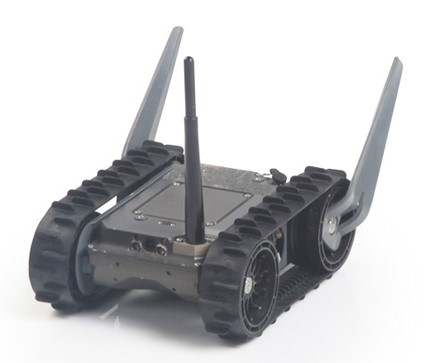
\includegraphics[width=1.0\textwidth]{FirstLook.jpg}}
            \caption{Endeavor Robotics 110 FirstLook \cite{endeavor}}
        \end{subfigure}
        \begin{subfigure}[h]{0.5\textwidth}
            \centerline{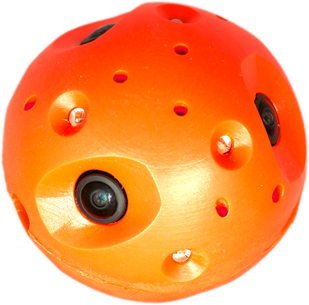
\includegraphics[width=0.8\textwidth]{bounce_img.png}}
            \caption{Bounce Imaging Explorer \cite{bounceImaging}}
        \end{subfigure}
\caption{Robotic Situational Awareness Devices}
\label{robocop}
\end{figure}
\par
These devices contain simple wireless video streaming technology, allowing for remote visual surveillance. Although a video stream is an effective strategy for simple surveillance, this method of gathering information has room for improvement. This project investigated the extraction of information such as object positioning and localization from a camera-based sensor suite in real time, allowing for more comprehensive situational observation. One method of performing this process is through the use of Simultaneous Localization and Mapping, or SLAM. 
\par
SLAM is a technique of mapping an unknown environment with respect to an agent, and can be performed using a wide variety of sensors and computational methods. This technique is a common area of research in the fields of image processing and high-speed computing, and has been applied mainly to autonomous vehicles. Most current SLAM implementations rely on the use of a sensor suite connected to a computer or System on Chip (SoC) computing device. 
\par
One type of technology useful for performing the high speed data processing necessary for an embedded SLAM device is a Field Programmable Gate Array, or FPGA. FPGAs consist of digital circuitry that is designed to be user-configured, allowing for the creation of completely customized digital hardware. FPGAs are especially useful for parallelized data processing, posing potential real-time advantages over standard computing or microcontroller technology. Although FPGA technology is highly applicable to performing SLAM-like tasks, there are currently few existing products that use FPGAs for this purpose. 
\par
This project explored the viability of an FPGA-based real-time SLAM sensor suite as a replacement for standard video cameras on existing situational awareness systems. This sensor suite utilized data from stereo camera modules, a scanning laser rangefinder, and an Inertial Measurement Unit (IMU) to create a real-time depth-augmented video feed and a 2D floorplan from the device's field of view.
\par
The following chapters detail the creation of this sensor suite, beginning with an exploration of relevant technology and prior work. Next, the overall system design of the project is included with a system block diagram. Then, each individual sensor’s implementation is explored in more detail. Methods for processing and combining sensor data to produce the intended 2D floorplan and 3D map visualizations are included. Comprehensive test results are then examined in detail for all sensors and main algorithms used. Lastly, conclusions and recommendations for future improvements are presented. 
 %%%% Introduction %%%%

\newpage
\section{Background}
The initial research portion of this project focused on learning more about different remote situational awareness products and how they may have been improved using existing technology, eventually leading to a set of overall project goals.

\subsection{Remote Situational Awareness Products}
Many situational awareness devices consist of remote-controlled throwable robots with wireless video-streaming capability. One such example is the 110 FirstLook by Endeavor Robotics, seen in Figure \ref{robocop}a. This device is a throwable, rugged robot that streams real-time video of its surroundings, and is used to investigate dangerous locations and hazardous material while keeping its operator out of harm's way. The 110 FirstLook has four day and night cameras, and also supports two-way audio. The device is remotely controlled by a tablet operator control unit, and is currently in use for military applications \cite{endeavor}.
\par
Similar to the 110 FirstLook, the Bounce Image Explorer is a throwable camera ball that wirelessly transmits a 360$^\circ$ real-time video stream of its surroundings. The Bounce Image Explorer can be seen in Figure \ref{robocop}b. The Explorer processes input from six monochrome WVGA camera modules, and outputs a video stream that can be accessed from a tablet or smartphone. This device is currently in a trial phase with United States Law Enforcement \cite{bounceImaging}. 
\par
A more commercial remote situational awareness device is the Serveball Squito\textsuperscript{TM} \cite{serveball}. Squito is a wireless, throwable, 360$^{\circ}$ panoramic camera that implements target detection to produce a stabilized output video stream. This device is shown in Figure \ref{squito} below.

\begin{figure}[H]
	\centerline{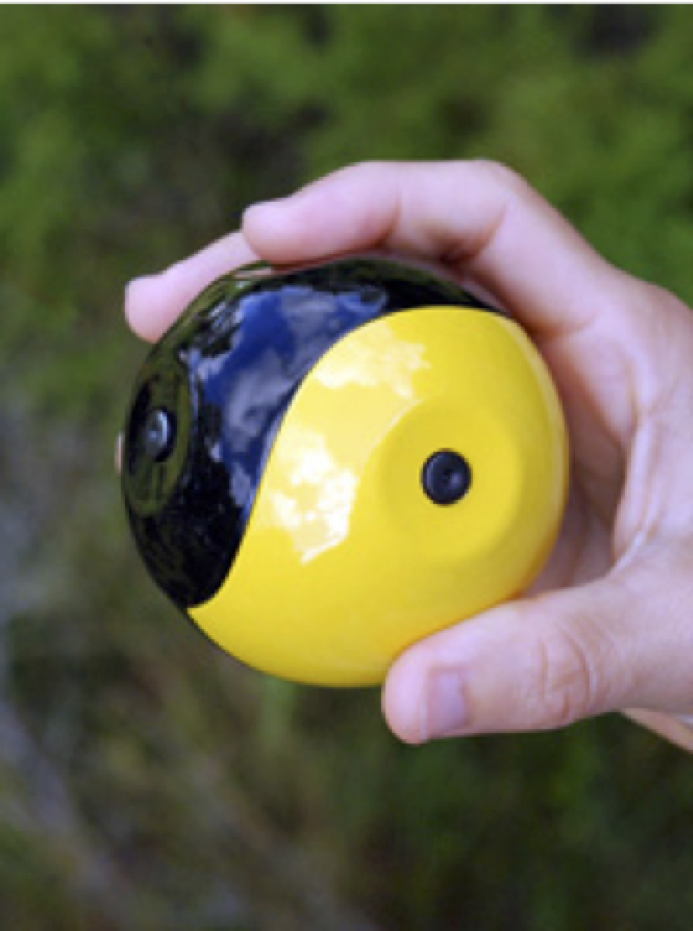
\includegraphics[width=0.3\textwidth]{serveball_squito.png}}
	\caption{Serveball's Squito \cite{serveball}}
	\label{squito}
\end{figure}

Squito utilizes a microprocessor receiving input from a fiber optic camera interface, as well as orientation and position sensors, in order to transmit a real-time stabilized video of its surroundings. The image in Figure \ref{squito_io} shows the input from the Squito's four camera inputs on the left, and a corresponding stitched output on the right. The device is still in the prototype stage, and has received interest from the first responder community. 
\par
\begin{figure}[H]
	\centerline{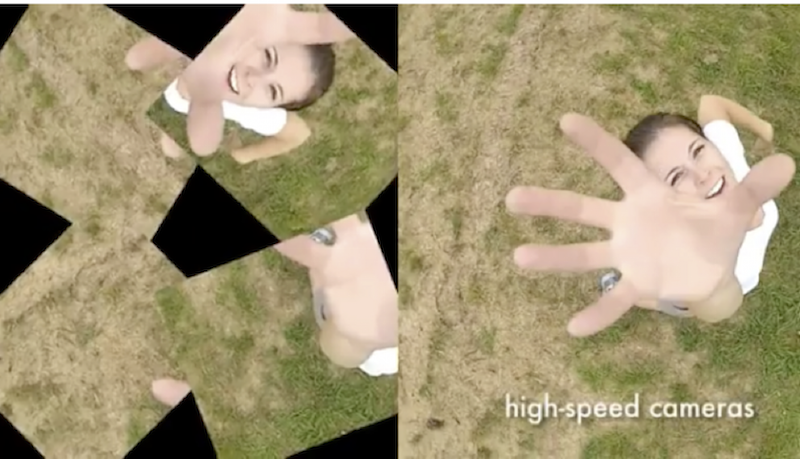
\includegraphics[width=0.6\textwidth]{serveball_io.png}}
	\caption{Serveball's Squito Input and Output \cite{serveball}}
	\label{squito_io}
\end{figure}
\par
The 110 FirstLook, Explorer, and Squito are all examples of remote situational awareness products that contain basic controls and real time video streaming outputs. Using additional image processing in the form of Simultaneous Localization and Mapping, the outputs of each of these devices could be improved to create comprehensive situational awareness. 

\subsection{Simultaneous Localization and Mapping}
As mentioned in the previous chapter, Simultaneous Localization and Mapping is the technique of mapping an unknown environment with respect to a localized agent. SLAM is especially useful for autonomous systems and remote observation, as it can be used for situational analysis and response. Recent research in the field of SLAM has focused on making these systems more portable.
\par
One application of such a system was a proof of concept of camera-based SLAM implementation for feature identification presented by Andrew Davison of Oxford University \cite{davison}. This system was handheld, and relied on a computer using a 2.2 GHz Pentium processor connected to a single camera and laser rangefinder. This system implemented edge detection on a known environment, and produced a real-time video output containing a 3D feature localization plot. An output frame from the device is shown in Figure \ref{rtSLAM}.

\begin{figure}[H]
	\centerline{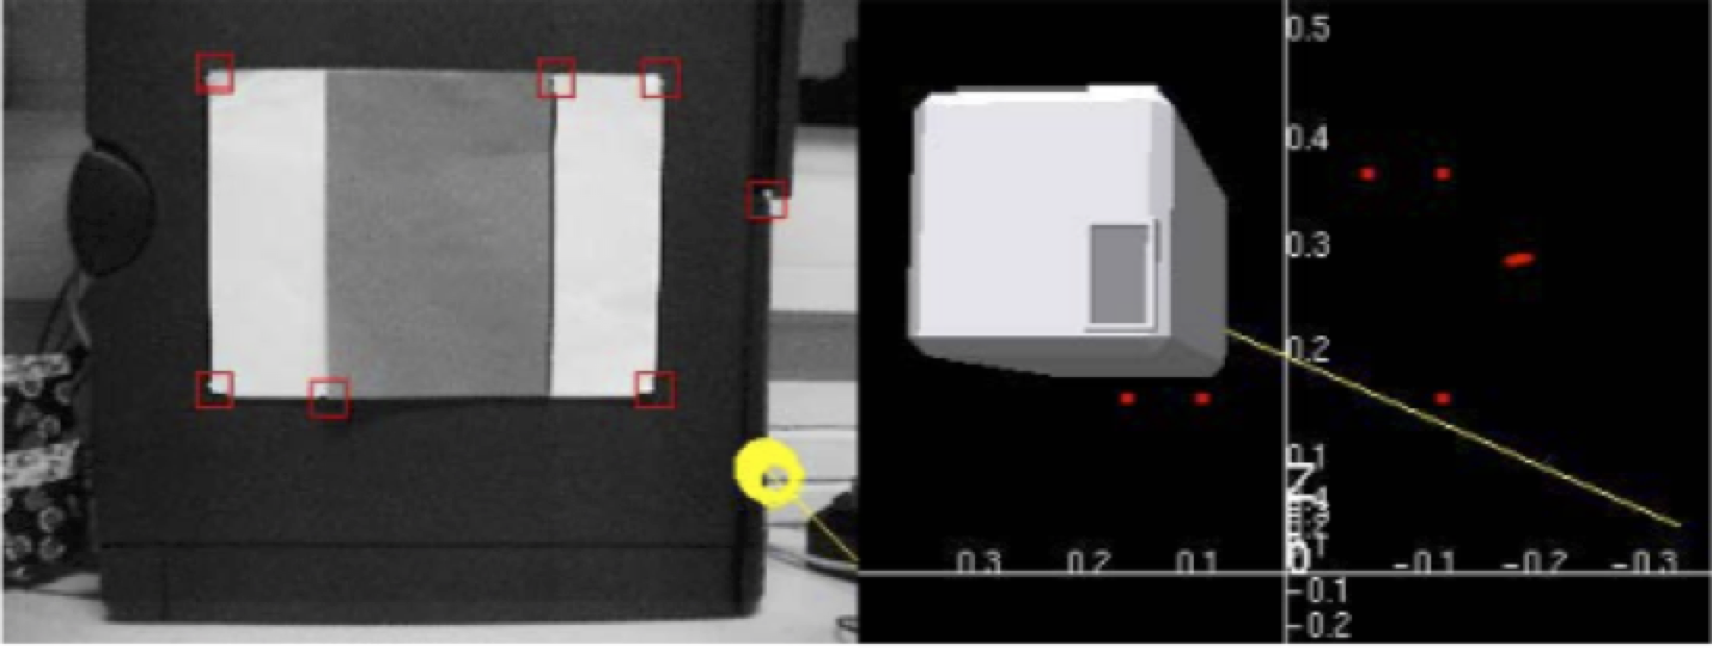
\includegraphics[width=0.8\textwidth]{real_time_SLAM.png}}
	\caption{Real-Time SLAM with a Single Camera \cite{davison}}
	\label{rtSLAM}
\end{figure}

The left image in Figure \ref{rtSLAM} shows 6 points of a paper target that were input to the system as prior knowledge, along with successfully marked identifying features (marked as red squares), and another identifying feature that was not marked for measurement (marked by a yellow circle). The frame on the right is a localization plot that displayed the relative positions of all red squares detected by the device.
\par
Along with identifying features of interest, SLAM image processing techniques are also used for depth estimation. The process of estimating depth from imagery is known as disparity mapping. Disparity mapping algorithms are used to calculate the similarities between stereo camera image pairs, and to convert said similarities to relative depth measurements. Disparity mapping is useful for situational awareness because it is used to determine the exact locations of all objects within a sensor suite's field of view.
\par
University of Bologna researchers Stefano Mattoccia and Matteo Poggi have worked to implement a real-time disparity mapping algorithm on an FPGA, and an example of a disparity image from this implementation is shown in Figure \ref{disparity_example} \cite{mattoccia}. Using their stereo disparity implementation, the researchers were able to generate real-time video showing the relative locations of objects within the device's field of view. The relative distance from the device to a given object was displayed using a color gradient, with nearer objects shown in brighter colors. Based on this depth information, it was also possible for the researchers to detect objects located within the field of view of the stereo imaging system, as shown in Figure \ref{disparity_example}. This implementation was extremely applicable to situational awareness systems, as it allowed for the localization of objects and creation of 2D slices of an area in real-time using only two camera sensors.
\par
\begin{figure}[H]
	\centerline{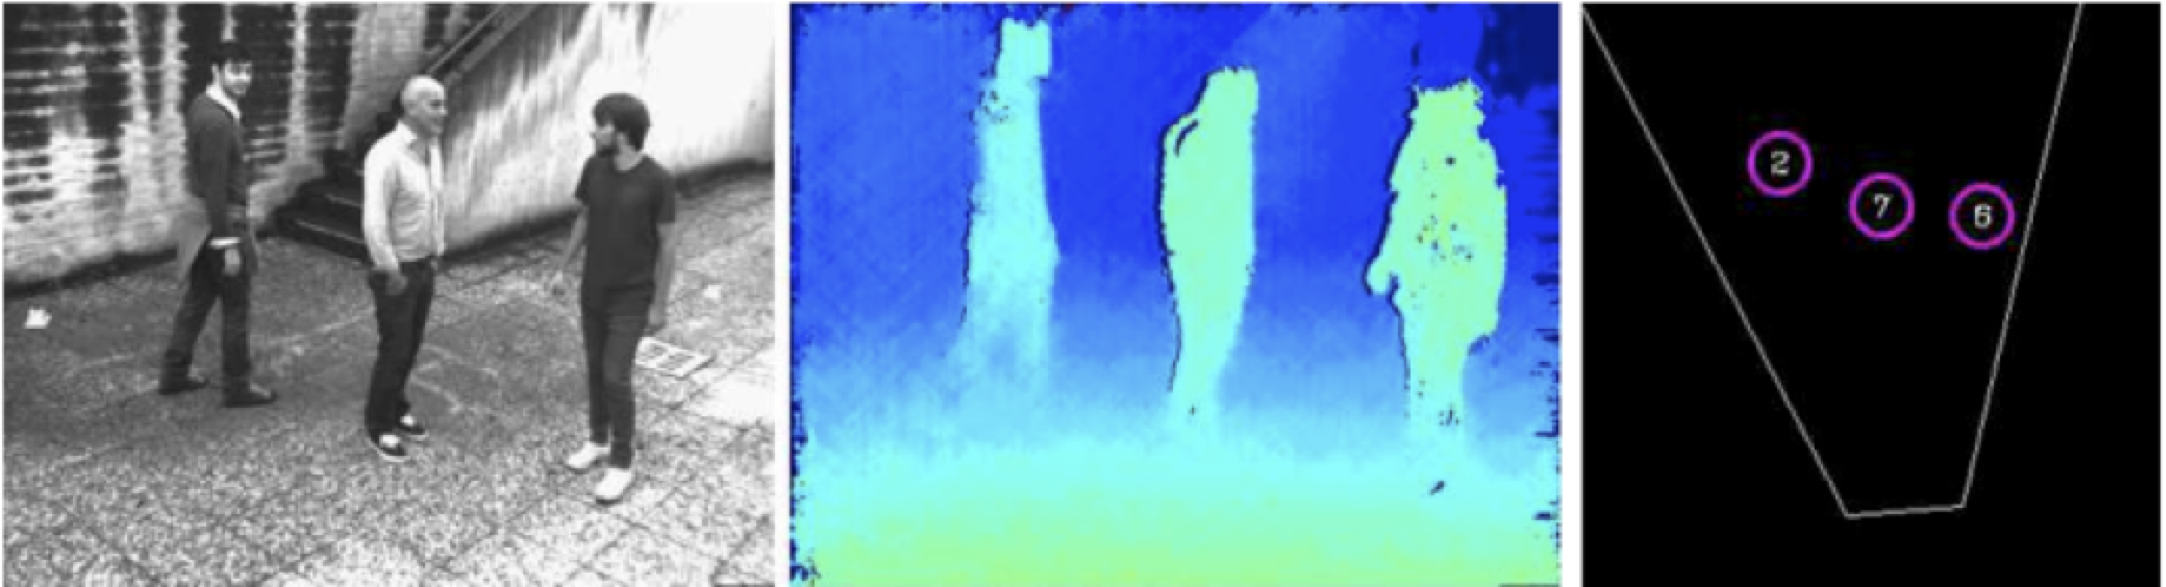
\includegraphics[width=0.9\textwidth]{disparity_example.png}}
	\caption{From Left to Right: Original Image, Disparity Map, Object Detection Results \cite{mattoccia}}
	\label{disparity_example}
\end{figure}
\par
A major concern with calculating disparity in real time is image processing speed. In the case of the implementation shown above, the parallelized data processing capabilities of FPGA hardware were used to address these concerns. The successful creation of this system demonstrated that FPGAs are useful for complex image processing applications \cite{mattoccia}. 

\subsection{The Zynq Evaluation and Development Board (ZedBoard)}
The FPGA platform used in this project was the Zynq Evaluation and Development Board, or ZedBoard. The ZedBoard is a low-cost development board containing a Xilinx Zynq-7000 All-Programmable SoC, and is shown in Figure \ref{zedboard_pic}.

\begin{figure}[H]
	\centerline{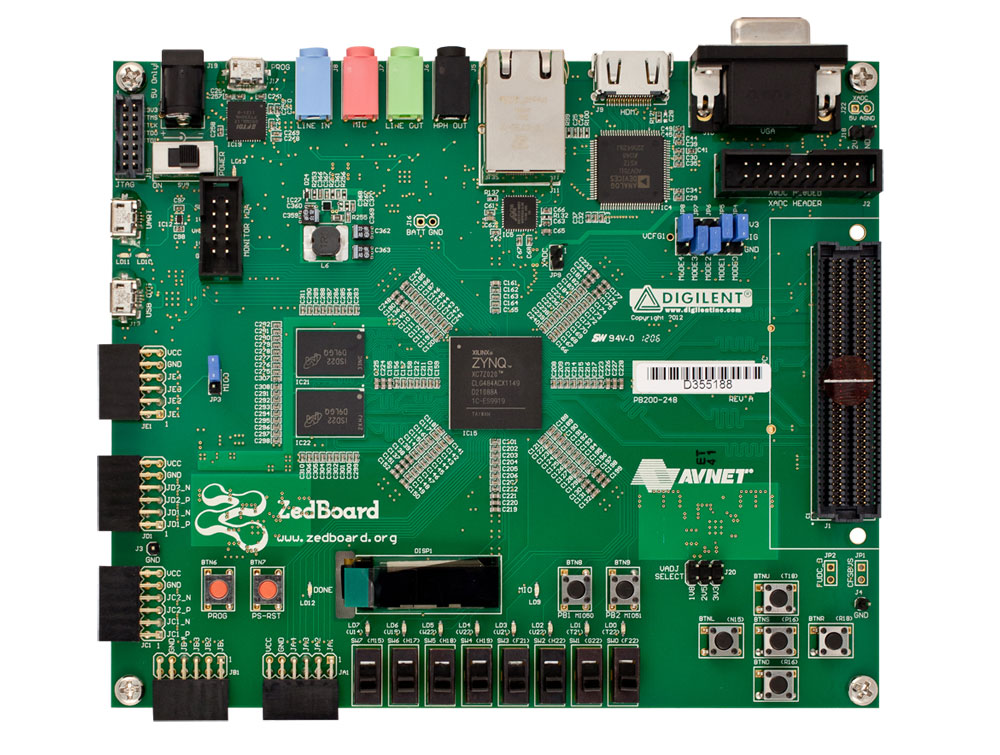
\includegraphics[width=1\textwidth]{ZedBoard.jpg}}
	\caption{The Avnet ZedBoard \cite{zedboard_photo}}
	\label{zedboard_pic}
\end{figure}

The Xilinx Zynq-7000 SoC consists of a dual-core ARM Cortex A9 processor coupled with Xilinx Artix-7 FPGA fabric. The ARM Cortex A9 processor uses a dedicated 33.3333 MHz clock source, while the onboard 100 MHz oscillator supplies the Programmable Logic (PL) clock. The Zynq-7000 SoC contains 85,000 programmable logic cells with 140 36K Block RAM modules. The ZedBoard also features 5 Pmod IO ports, 8 LEDs, 8 switches, 7 push buttons, a USB UART port, and a VGA port \cite{zedboard_datasheet}. These are shown in the ZedBoard's block diagram in Figure \ref{zedboardbd}.

\begin{figure}[H]
	\centerline{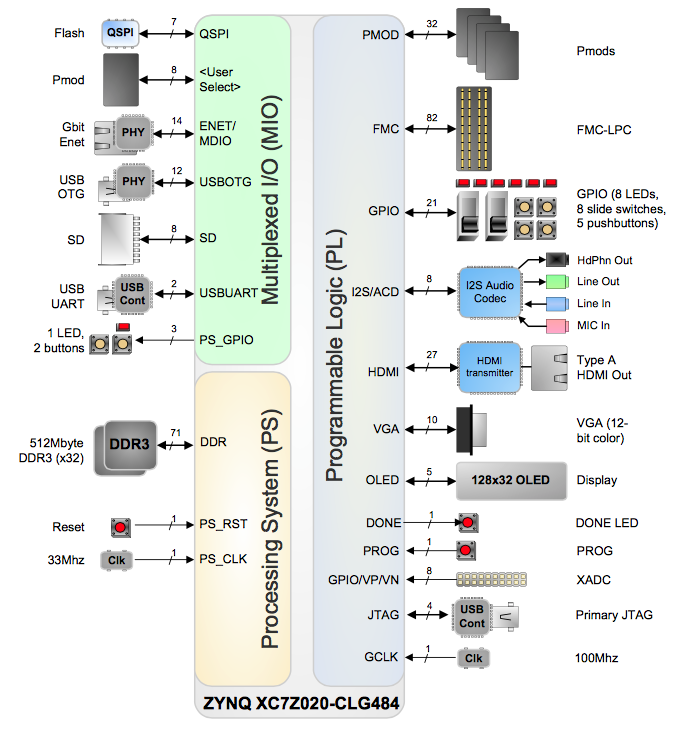
\includegraphics[width=0.85\textwidth]{ZedBoardBD.png}}
	\caption{ZedBoard Block Diagram \cite{zedboard_datasheet}}
	\label{zedboardbd}
\end{figure}
\par
As our research progressed, it became evident that FPGAs were a viable solution for implementing real-time situational awareness algorithms on a compact scale. For the purposes of this project, we decided to interface the ZedBoard with a stereo camera pair to gather disparity depth information on an area, and supplement that data with digital compass and rangefinder readings to produce detailed maps of the sensor suite's surroundings in real time. The implementation scheme for this device is detailed in the following chapter.





 %%%% Background %%%%

\newpage
\section{System Design}
Overall, the proposed system has been reduced to the functional blocks shown in Figure \ref{systemBD} below. On the input side of the system, the two stereo cameras are physically connected to two video memory buffers, and the camera controls and video memory buffer data are accessed through programmable logic on the Zynq processor.  Since the rangefinder and IMU modules each communicate with UART and SPI interfaces, respectively, each are connected directly to the Zynq's dual-core ARM processor. Both sensors may then be communicated with using Xilinx's built-in ARM peripheral drivers, reducing overall implementation time. Note that an I$^2$C controller is also included as a peripheral for the ARM processor, allowing for communication with each camera's control registers. 
\par
\begin{figure}[H] 
	\centerline{
	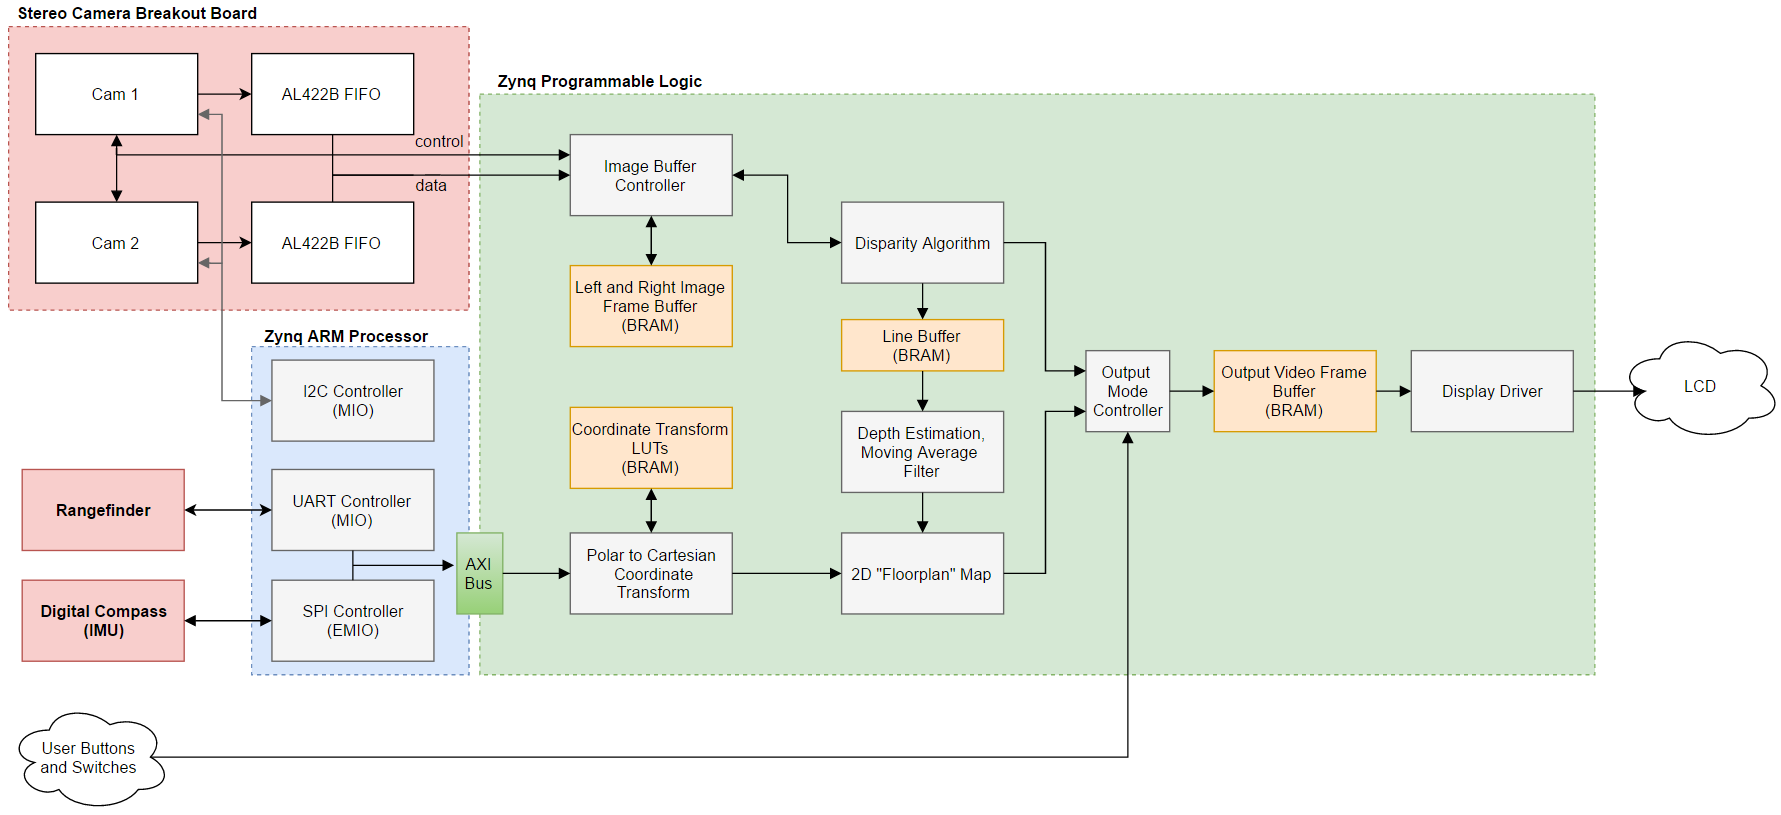
\includegraphics[width=1.25\linewidth]{full_blockdiag.png}
	}
	\caption{System Block Diagram}
	\label{systemBD}
\end{figure}
\par
In terms of stereo camera data processing, the first stage of programmable logic consists of a dual image buffer controller used for triggering image captures and reading image data into local memory on the ZedBoard. A disparity module then reads in image data from local memory, and calculates the relative offset between objects contained in the stereo image pair. A portion of this data is then stored in local memory for correlation with data from the 2D scanning laser rangefinder. Depending on the position of the ZedBoard's user input switches, the output from the disparity algorithm is also passed to a video frame buffer and displayed via VGA. 
\par
In order to correlate disparity data with the 2D depth information from the scanning laser rangefinder, several horizontal lines of pixel data from the disparity algorithm are averaged together. This single line of depth information can be compared to the single line of depth information from the rangefinder. However, due to differences in the field of view of each sensor, the depth information is passed through a moving average filter before being correlated with rangefinder data. 
\par
Data from the scanning laser rangefinder and IMU modules is pre-processed in programmable software, allowing for the estimation of sensor rotation relative to the IMU's compass heading.  A custom AXI peripheral bus is then used to pass data from the programmable software to the programmable hardware. At this stage, a pair of lookup tables are used to convert the rangefinder data from Polar to Cartesian coordinates, and the modified data is correlated with depth estimation data from the disparity algorithm. Depending on the status of the ZedBoard's user switches, the 2D floorplan map created using the combined sensor data is then passed to the output video buffer for external display. 

\newpage
\section{System Implementation}
After deciding that the proof of concept sensor suite would rely on a scanning laser rangefinder, IMU, and stereo camera interface, research was then performed in order to determine what specific sensors to use, as well as the operating modes of each chosen sensor. 
\subsection{Rangefinder Operation}
A rangefinder is a device that estimates the distance of the objects closest to it. Because this sensor suite was intended to traverse unknown locations and create a 2-dimensional map, data accuracy, precision, and reliability were vital design requirements.

\subsubsection{Selection}
The project's rangefinder selection depended on the following criteria: field of vision, maximum sensible depth, accuracy, precision, and cost. Many of the rangefinders limited by the project's budgetary restrictions were severely lacking in at least one of our project's vital criteria. However Professor Duckworth, and WPI's Electrical and Computer Engineering and Robotics Engineering Departments generously donated the URG-04LX Scanning Laser Rangefinder for the purpose of this project. The URG-04LX, shown in Figure \ref{rangefinder_pic}, is a durable, lightweight piece of equipment that has a field of view of $240^\circ$ and can sense objects up to 4 meters away with an accuracy to within 10 millimeters, which was perfect for our application \cite{urg04lx_specifications}.

\begin{figure}[H]
	\centerline{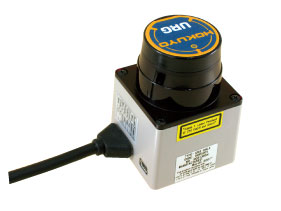
\includegraphics[width=0.5\textwidth]{urg_top.jpg}}
	\caption{URG-04LX Scanning Laser Rangefinder \cite{rangefinder_photo}}
	\label{rangefinder_pic}
\end{figure}

\subsubsection{Communication} \label{sssec:rangefinder_communication}
The URG-04LX rangefinder used the Recommend Standard (RS) 232C protocol via Universal Asynchronous Receiver/Transmitter (UART) communication. RS-232 is a form of differential serial data transmission which recognizes a digital logic high from -3V to -25V, and a digital logic low from +3V to +25V \cite{rs232}.
\par
Since the ZedBoard's Peripheral Module (Pmod) connectors supported UART communication, the rangefinder was communicated with using a Pmod IO connector. The ZedBoard's Pmod connectors used the Transistor-Transistor Logic (TTL) protocol, which is a form of non-differential serial data transmission that recognizes a logic high of +3V to +5V and a logic low of 0V \cite{ttl}. Since TTL has different logic levels than RS-232, these protocols were incompatible and did not recognize each other. Figure \ref{ttl_rs232_pic} shows a timing diagram of both RS-232 and TTL communication protocols.

\begin{figure}[H]
	\centerline{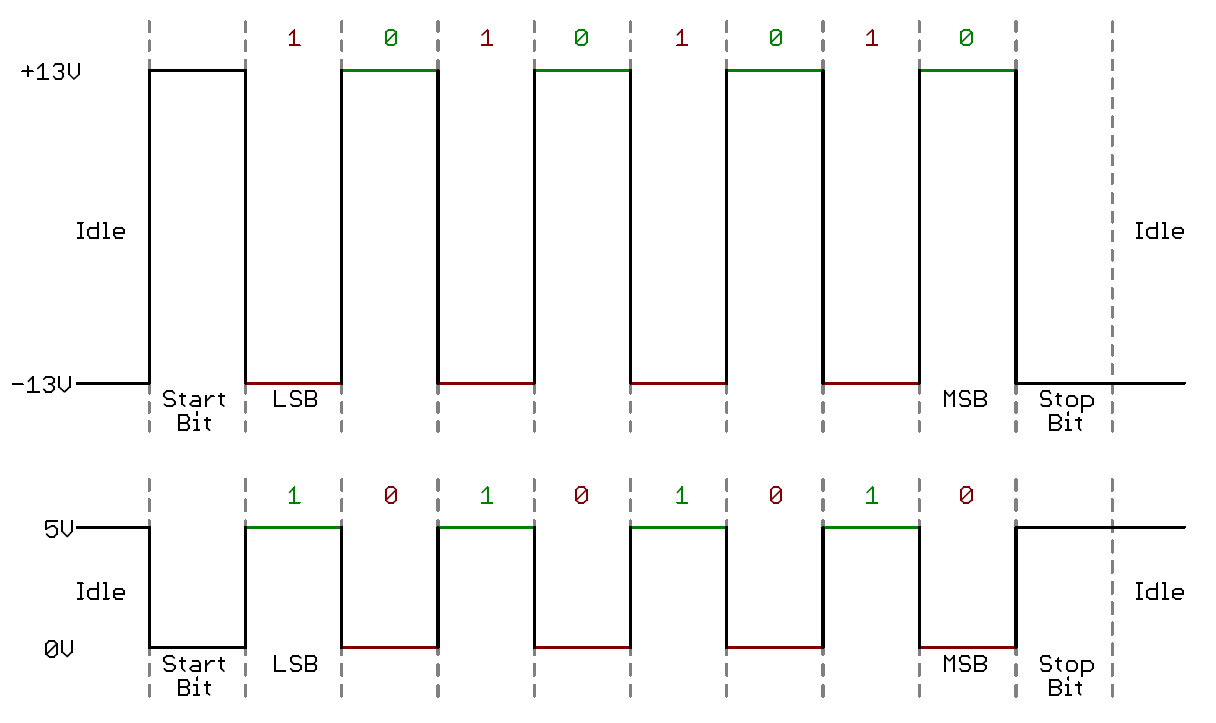
\includegraphics[width=0.9\textwidth]{ttl_rs232.png}}
	\caption{Timing Diagram of RS-232 (top) and TTL Communication Protocols \cite{ttl}}
	\label{ttl_rs232_pic}
\end{figure}

To address these logic-level issues, an external RS-232 to TTL converter board was needed to allow the rangefinder to communicate with the ZedBoard. The converter's TTL side was connected to the ZedBoard's Pmod connector, and the RS-232 side was connected to the rangefinder. For ease of connection and testing, the 9-pin DSUB RS-232 connector was connected to an RS-232 breakout board so that the pins were easily accessible. Figure \ref{rs232_ttl_breakout} shows the RS-232 to TTL converter attached to the RS-232 breakout board.

\begin{figure}[H]
	\centerline{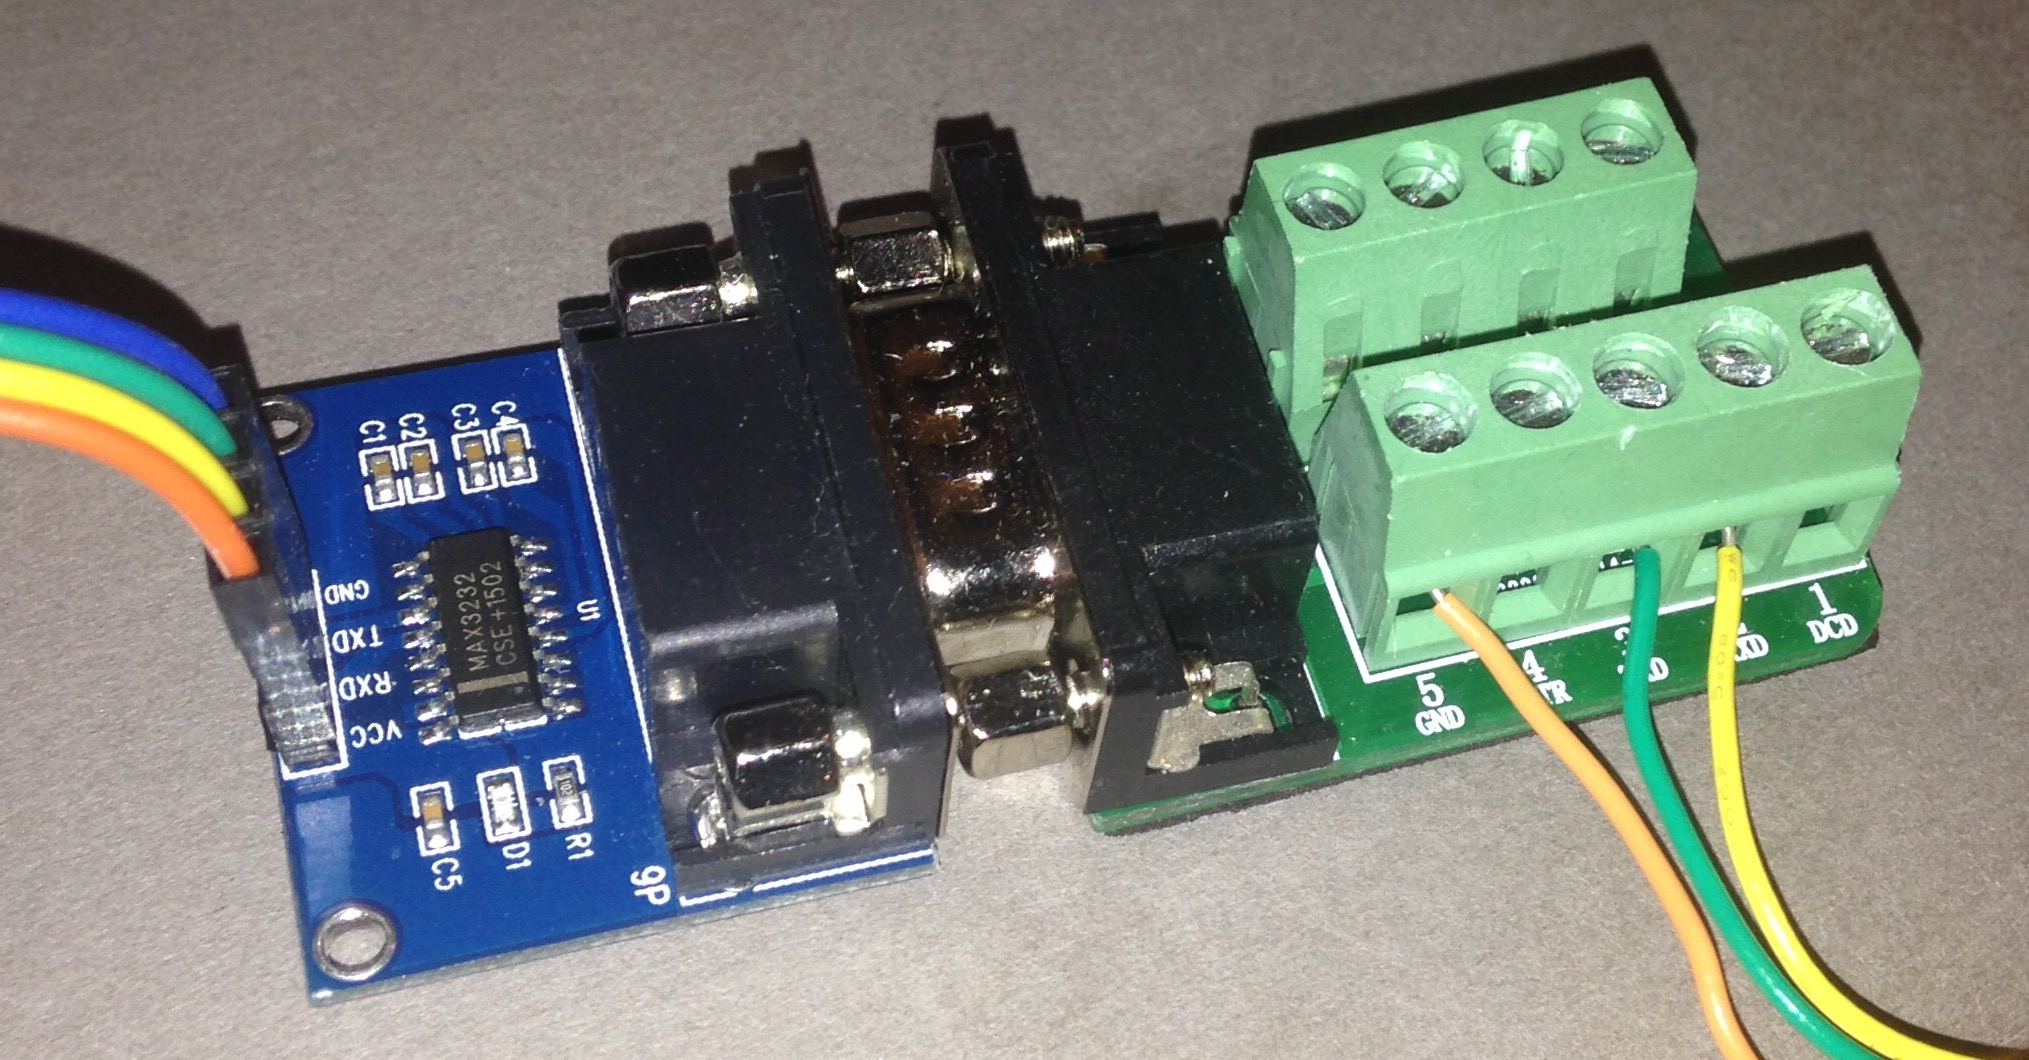
\includegraphics[width=0.6\textwidth]{rs232_ttl_breakout.png}}
	\caption{RS-232 to TTL Converter with RS-232 Breakout Board}
	\label{rs232_ttl_breakout}
\end{figure}

Although the ZedBoard's Pmod connectors were sufficient for UART communication with the URG-04LX, the power specifications were not compatible; the Pmod connectors output 3.3V but the rangefinder required 5V \cite{zedboard_datasheet, urg04lx_specifications}. Thus, the rangefinder was powered externally by a lab bench power supply.

\subsubsection{Commands}
The rangefinder defaulted to a communication speed of 19.2 kbps (19200 baud) and recognized four different commands: the version command, the communication speed setting command, the laser illumination command, and the distance data acquisition command \cite{urg04lx_datasheet}. The version command and the communication speed setting commands were both not used for the purpose of this project. The laser illumination command was used as a debugging tool to turn the laser on and off. The laser's status was displayed using a status LED on the rangefinder, so turning the laser on and off allowed for simple visual confirmation of successful communication. The distance data acquisition command was the primary command used in this project, as it was used for gathering new distance data from the rangefinder.
\par
The distance data acquisition command consisted of five different pieces that controlled the data output: 'G', the data starting point, the data end point, the cluster count, and either a line feed or a carriage return. The start point was the step of the area from where the data reading started, and the end point was where the data reading stopped. The data reading started at the start point and traversed counterclockwise until the end point. Figure \ref{rangefinder_fov} shows a top-down view of the rangefinder's field of vision with the steps labeled.

\begin{figure}[H]
	\centerline{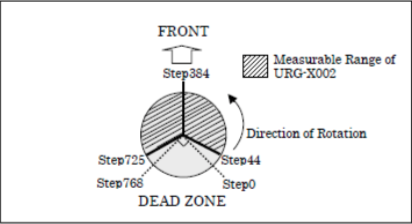
\includegraphics[width=0.7\textwidth]{rangefinder_fov.png}}
	\caption{Top-Down View of Rangefinder Field of Vision \cite{urg04lx_datasheet}}
	\label{rangefinder_fov}
\end{figure}

For this project, the beginning point was set to '000' and the end point to '768' to obtain the device's maximum coverage of $270^\circ$.
\par
The cluster count is the number of neighboring points that were grouped together as a cluster. In this implementation, the cluster count was set to '01' in order to have a cluster count of one data point.
\par
Putting all of these pieces together, the data acquisition command 'G00076801\textbackslash{}n' was obtained and transmitted from the ZedBoard to the rangefinder to request one scan of data. With the rangefinder's operation understood, an interface was created for connecting the ZedBoard to the rangefinder.





\subsection{Rangefinder Implementation}
With the data acquisition command tested and functioning properly, the rangefinder needs to be connected to the ZedBoard. Since the URG-04LX uses UART communication, there are a few reasonable options to create a UART controller on the ZedBoard.

\subsubsection{UART Options}
As the ZedBoard is such a powerful device, it has a few different options for controlling UART. A few of them are by controlling UART through linux, through a MicroBlaze soft-core processor, or through the Zynq-7000 Processing System. Running linux on the ZedBoard would use much of the board's valuable resources, and we would only be using a fraction of the capability provided by linux. The MicroBlaze soft-core processor would be a better alternative, but it runs in the programmable logic in the FPGA and is unnecessary when the ARM processor on the ZedBoard is unused \cite{microblaze}. Because of this, we decided to utilize the ARM processor on the ZedBoard by using the Zynq7 Processing System via Xilinx's Zynq-7000 Processing System Intellectual Property (IP) core.

\subsubsection{Zynq7 Processing System}
The ZedBoard SoC features a dual-core ARM Cortex-A9 MPCore processing system and Xilinx Programmable Logic. The Zynq7 Processing System IP core acts as a logic interface that integrates the Programmable Software (PS) with the Programmable Logic (PL), which allows access to both on-chip and external memory interfaces, to PL clocks, to many I/O peripherals, and even to extended I/O peripherals \cite{zynq7ps}. With all of this overwhelming functionality, the processing system is easy to customize, featuring a simple user interface, once it is added into a project's block design. The user interface can be used to change the processing system's activated features. Figure \ref{zynq7ps_pic} below shows the processing system customization window.

\begin{figure}[H]
	\centerline{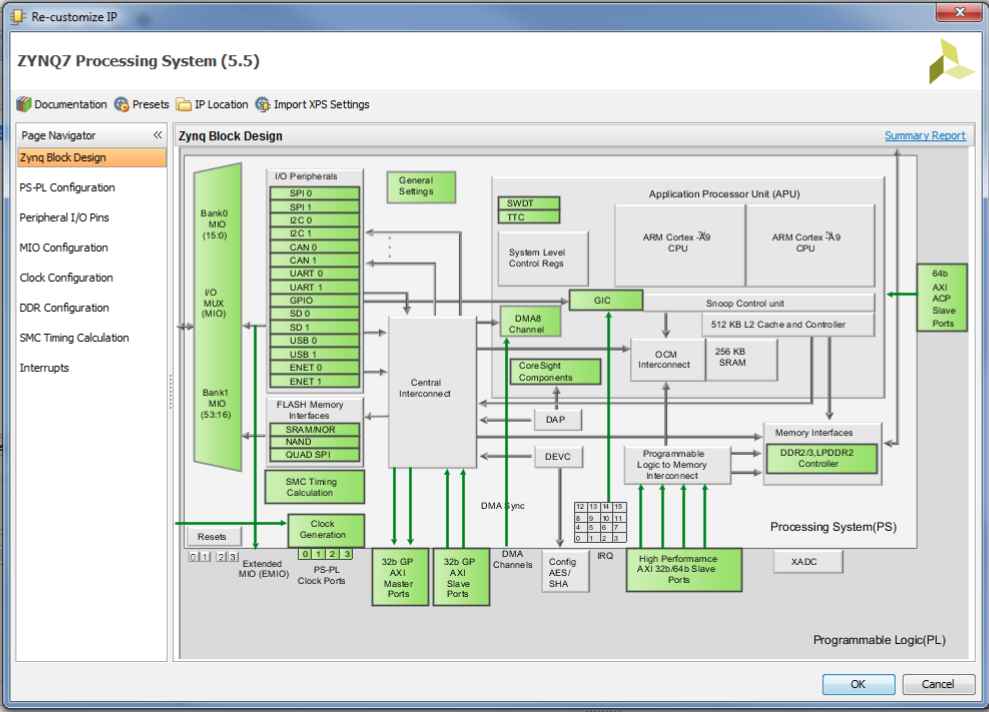
\includegraphics[width=1\textwidth]{zynq7ps.png}}
	\caption{Zynq7 Processing System Customization Window \cite{zynq7ps}}
	\label{zynq7ps_pic}
\end{figure}

In the figure above there are two options for UART shown: UART0 and UART1. The functionality of UART0 and UART1 are nearly identical, except that UART1 has the capability of being routed to the ZedBoard's USB UART port, which is not compatible with the rangefinder \cite{zedboard_datasheet}. So, we arbitrarily chose UART0 and routed the signals to MIO10 and MIO11, which correspond to the ZedBoard's PS Pmod, JE.
\par
After choosing UART0 and configuring the MIO pins, the Baud Rate needs to be configured such that it corresponds with the rangefinder's default communication speed, 19200 Baud \cite{urg04lx_datasheet}. This can be done in the processing system's customization window under PS-PL Configuration on the sidebar in Figure \ref{zynq7ps_pic}. Figure \ref{zynq7ps_baud_pic} below shows the PS-PL Configuration window.

\begin{figure}[H]
	\centerline{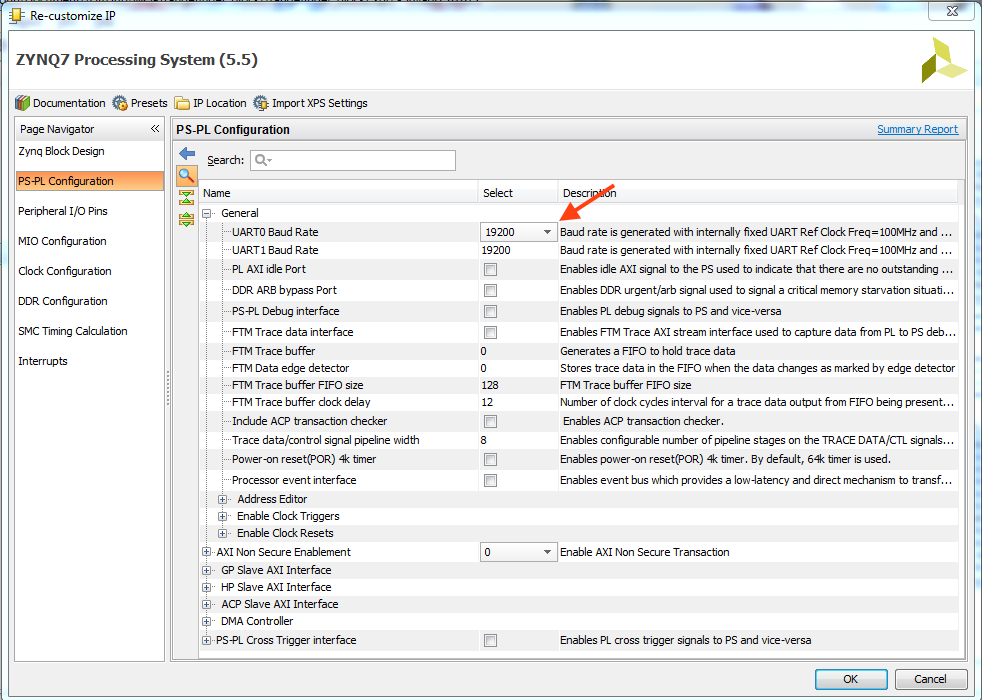
\includegraphics[width=1\textwidth]{zynq7ps_baud.png}}
	\caption{Zynq7 Processing System PS-PL Configuration Window}
	\label{zynq7ps_baud_pic}
\end{figure}

With the processing system customized in this fashion, the programmable logic's configuration is complete.

\subsubsection{PS-PL Communication / Creating Custom IP}
\label{sssec:ps_pl}
maybe break into two sections? one for ps-pl and talk about what AXI is and why we need to use it, and then in the testing and results section make a second one about how we needed to create custom axi peripherals? whatever works best
I HAVE NO IDEA WHAT TO WRITE FOR THIS
\subsection{Rangefinder Data Processing}
With the communication between the ZedBoard and rangefinder, and between the PS and PL functioning properly the data processing can begin.

\subsubsection{Programmable Software}
The Programmable Software (PS) is responsible for all of the communication with the rangefinder, in addition to formatting the data before it is sent to the Programmable Logic.
\par
The distance data acquisition command is transmitted by the PS when it receives a signal from the PL. Once the command is sent, there are two different pieces of information that the software needs to capture: the distance data and the step count. The rangefinder transmits the distance data half a data point (one character) at a time, but it does not transmit the step count. As such, the software receives the distance data one character at a time, so the first character is stored in a buffer until the second character is received. Once the second character is received the distance data buffer is updated to hold both characters, the step count is incremented, and then both are sent to the PL by writing them to the memory location referenced by it, as discussed in Section \ref{sssec:ps_pl}.

\subsubsection{Programmable Logic}
The Programmable Logic (PL) is responsible for all data processing, block memory manipulation, and outputting to VGA.
\par
The rangefinder encodes each data point before transmitting it. The uncoded data point is expressed with 12 bits, in order to cover the device's maximum distance of 4095 millimeters. The 12-bit data is separated into two 6-bit data points, and 30\textsubscript{16} is added to each. The resultant data point is comprised of two ASCII characters \cite{ascii}. The decoding process takes place in the PL, and is the inverse of encoding where 30\textsubscript{16} is subtracted from each character and then they are merged together \cite{urg04lx_datasheet}.
\par
Since the rangefinder provides the distance away from an object and the angle at which it was detected, the data is essentially expressed in the polar coordinate system \cite{polar_coordinates}. We will be outputting our data on a VGA screen which expresses data in the rectangular (Cartesian) coordinate system, so we must convert from polar to rectangular coordinates. This is accomplished by using the step number, which corresponds to an angle around a circle as shown in Figure \ref{rangefinder_fov}.
\par
Converting from polar to rectangular coordinates requires basic trigonometry. Luckily, Xilinx supports a few options for performing complex math operations in the PL: a Coordinate Rotational Digital Computer (CORDIC) function, multiplier IP blocks, or Lookup Tables (LUTs). Due to latency concerns and ease of integration, we decided to implement a LUT with a multiplier instead of a CORIC function. The values in the LUT will be used to extract the horizontal and vertical components from the polar coordinate. Taking advantage of a circle's symmetry, the LUT only needs to hold values 256 values, which correspond to the amount of rangefinder data steps in one quadrant of a circle. Each step value is manipulated such that it corresponds to two addresses in the LUT: one for the horizontal scale factor, and one for the vertical scale factor.
\par
The LUT was set up in Vivado using a read-only BRAM IP core with a depth of 256, and was initialized by importing a coefficient file (.coe). The 256 values in the coefficient file were calculated by using Equation \ref{coe} for step values between 128 and 384, corresponding to one quadrant of a circle. Note that multiplying by 4096 equates to a 12-bit left shift, and is used to decrease error due to rounding in later data manipulation.

\begin{equation}
	\textrm{LUT}[step] = \sin((384-step)\times\dfrac{\pi}{180})\times4096
	\label{coe}
\end{equation}

Only one address in the BRAM can be read from at a time, but we require both a horizontal and vertical scale factor. To avoid read conflicts, the 256-address LUT was split into two 129-address LUTs, where one LUT corresponds to $0^\circ{}\leq{}\theta{}\leq45^\circ$, and the other corresponds to $45^\circ{}\leq{}\theta{}\leq90^\circ$. Separating the LUT to solve this problem takes advantage of the property that sine and cosine are $90^\circ$ out of phase with each other\footnote{This process could have been avoided by setting up the BRAM in a True Dual Port ROM configuration, so that there are two separate, individually addressable address busses for the same BRAM block.}. The code for the coefficient files can be found in Appendix \ref{coe_file}.
\par
Once the LUT was customized, the BRAM IP Wizard window specifies the BRAM's latency. In this case, once the addresses are calculated there is a latency of 2 clock cycles before the data from the LUT is valid. Once the horizontal and vertical data is valid, each is multiplied by the decoded polar coordinate data point by being input to a Multiplier IP block which, in this case, has a latency of 4 clock cycles. This transformation changes the data from polar to rectangular coordinates. After this step, the data is shifted back in a manner such that the data points will be able to fit on a VGA screen with resolution $640\times480$ pixels. Next the data needs to be localized to the device's location, so the x- and y-coordinates are shifted by the device's location. After this step, the x- and y-location accurately reflect the distance data localized to the device.
\par
With proper x- and y-coordinates, the data is ready to be stored in memory. Another BRAM IP was created for the VGA control. Our VGA resolution is $640\times480$, so our VGA BRAM requires 307,200 addresses. This BRAM IP was customized to function in the write-first, dual port configuration. We implemented this BRAM module such that one port is a write-only port using our 100 MHz clock, and the other is a read-only port using our 60 Hz VGA clock. This BRAM IP avoids memory access conflicts by writing to memory before attempting to read. Our write address was calculated by using another Multiplier IP with Equation \ref{vga_wequation}.

\begin{equation}
	\textrm{write address} = (640\times{}y\textsubscript{location})+ x\textsubscript{location}
	\label{vga_wequation}
\end{equation}

\par
With the data stored in memory, it is ready to be output to a VGA screen. We implemented a VHDL $640\times480$ VGA controller model by Digilent, found in Appendix \ref{vga_controller} ADD ANOTHER APPENDIX FOR CODE, to control our VGA logic. In addition, the ZedBoard's VGA pins were configured in a constraints file (.xdc) to support 12-bit color resolution \cite{zedboard_datasheet}. Similar to Equation \ref{vga_wequation}, Equation \ref{vga_requation} was used to calculate the read address of the VGA BRAM IP.

\begin{equation}
	\textrm{read address} = (640\times{}v\textsubscript{count})+ h\textsubscript{count}
	\label{vga_requation}
\end{equation}




\subsection{PS-PL Communication} \label{ssec:ps_pl}
Communication between the Programmable Logic (PL) and Programmable Software (PS) was implemented so that data was able to traverse between the ARM processor and the FPGA fabric on the SoC. This process was configured in Vivado with the use of an Advanced eXtensible Interface (AXI) bus.

\subsubsection{Advanced eXtensible Interface (AXI)}
AXI is a type of on-chip interconnect specification intended for transaction based master-to-slave memory mapped operations, which made it perfect for PS-PL communication. These AXI busses are integrally involved in most Xilinx IP cores and contain many wires with sophisticated logic. Instead of attempting to interface with AXI by creating these signals, a custom IP AXI Peripheral was created that abstracted away the complications of AXI communication.

\subsubsection{Creating Custom IP} \label{sssec:creatingCustomIP}
For this project, a custom IP module was created to serve as an AXI Peripheral. As an AXI Peripheral, this IP block was able to communicate with any other Xilinx IP blocks that use AXI. For the purpose of this project, the custom IP block uses its AXI bus to communicate with the Zynq7 Processing System. The custom IP was created in Vivado under Tools $\rightarrow$ Create and Package IP. The IP was set up as an AXI Peripheral, with four 32-bit wide memory registers attached to the AXI bus.
\par
Once the bare IP AXI peripheral was created, the custom IP's auto-generated files were edited to allow for memory registers in the design's custom logic to be wired to the AXI bus. In the auto-generated file for the AXI interface, several lines of code were edited in order to connect the AXI peripheral's input and output channels to custom logic. The IP was customized for the use of four memory registers, but only two were used: one for writing data to the PS, and the other for reading from the PS. 
\par
To write to the PS, the AXI output register data was wired to a register in the custom logic that held the data to be sent to the PS. This is done in the AXI read address $case$ statement that decodes addresses for reading registers. This can be seen on line 368 of our edited auto-generated custom IP code, shown in Appendix \ref{customIPaxi}. In the PS, a Xilinx built-in memory access function was used to read the data from the AXI output register, shown on line 130 of the programmable software in Appendix \ref{ps_code}.
\par
To read from the PS, the data stored in the AXI's input register was wired to a register in the custom logic. This was done in the AXI write address $case$ statement on line 239 of our edited auto-generated custom IP code, shown in Appendix \ref{customIPaxi}. In the PS, a pointer to the memory address of the AXI input register was read from to obtain the data from the custom logic, as seen on line 198 of the programmable software in Appendix \ref{ps_code}.
\par
In addition, other necessary I/O ports from the custom logic were created in the custom IP's top module. Our custom IP top module is found in Appendix \ref{customIPtop}. Advanced user logic was also implemented within the IP core through modular instantiation.
\par
Once the rangefinder's implementation into the system was complete, the digital compass was interfaced to in order to rotate the rangefinder's data according to the sensor suite's compass heading.


\subsection{Inertial Measurement Unit (IMU) Operation}
An Inertial Measurement Unit (IMU) is a device that measures linear and angular momentum, as well as the direction of the magnetic field at a point in space. It accomplishes this by reading data from an accelerometer, gyroscope, and magnetometer respectively. 

\subsubsection{Selection}
Our project requires a sensitive IMU that is able to provide data that can be used to tell compass direction and change of position. Due to the time limitations and budgetary restrictions of this project, we chose the Pmod NAV IMU that provides 10-degree of freedom functionality through the LSM9DS1 3-axis accelerometer, 3-axis gyroscope, and 3-axis magnetometer, and the LPS25HB barometer \cite{lsm9ds1, lps25hd}. The Pmod NAV is shown in Figure \ref{pmodnav}.

\begin{figure}[H]
	\centerline{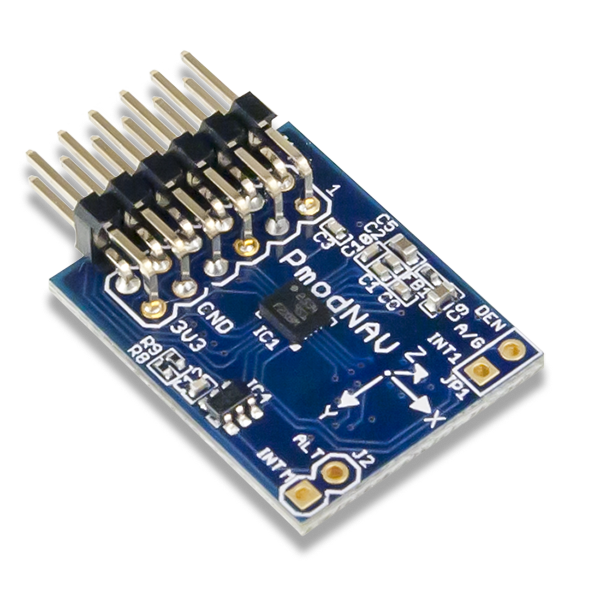
\includegraphics[width=0.5\textwidth]{pmodnav.png}}
	\caption{The Pmod NAV 10-Axis IMU \cite{pmodnav_ref}}
	\label{pmodnav}
\end{figure}

The Pmod NAV's simple Pmod connector makes the IMU easy to integrate into our design, as it can be fixed in position connected to the ZedBoard, and its communication is directly compatible, requiring no intermediate hardware.

\subsubsection{Communication}
The IMU supports two means of communication: Serial Peripheral Interface (SPI) and Inter-integrated Circuit (I\textsuperscript{2}C) Communication \cite{lsm9ds1}. However the magnetometer on the LSM9DS1 is not addressable by the I\textsuperscript{2}C bus. Since the magnetometer is needed to be able to tell compass direction, we chose to use SPI communication. The magnetometer sensor SPI protocol is shown in Figure \ref{magnetometer_spi}.

\begin{figure}[H]
	\centerline{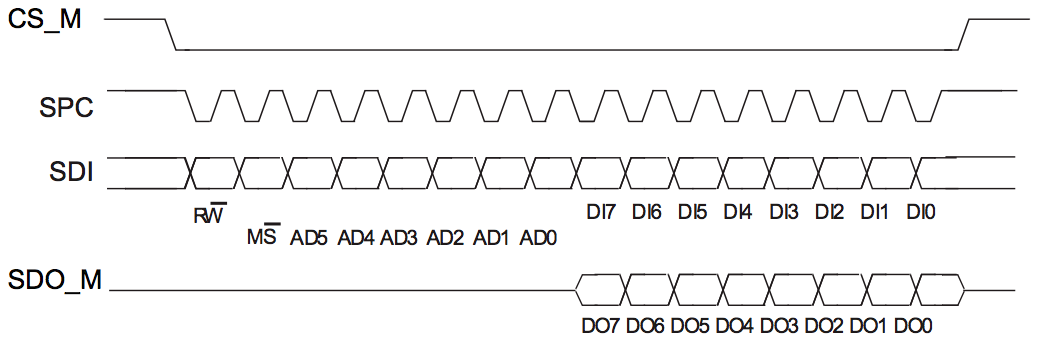
\includegraphics[width=1\textwidth]{magnetometer_spi.png}}
	\caption{Magnetometer SPI Read and Write Protocol \cite{lsm9ds1}}
	\label{magnetometer_spi}
\end{figure}

The CS\textunderscore{}M line is the magnetometer chip select and is an active low. It goes low at the beginning of the transaction and high at the end. The SPC is the clock controlled by the master. SDI and SDO\textunderscore{}M are the data input and data output lines, respectively. They are driven at the falling edge of SPC and should be captured at the rising edge \cite{lsm9ds1}.
\par
The register read and write commands are completed in 16 clock pulses. The first bit sent from the master, bit 0 or $R\overline{W}$, is the read/write bit. When data is read from the IMU this bit is sent to 1, otherwise it is set to 0. When bit 1, the $M\overline{S}$ bit, is set to 1 the address is auto-incremented, allowing for multiple read/writes to be completed in the same SPI sequence. Figure \ref{multiple_reads} shows a multiple byte SPI read protocol. Bits 2-7, the $AD$ bits, are the address bits transmitted MSB first. When in write mode bits 8-15, the $DI$ bits, are the data that is written to the device MSB first. When in read mode bits 8-15, the $DO$ bits, are the data that is read from the device MSB first \cite{lsm9ds1}.

\begin{figure}[H]
	\centerline{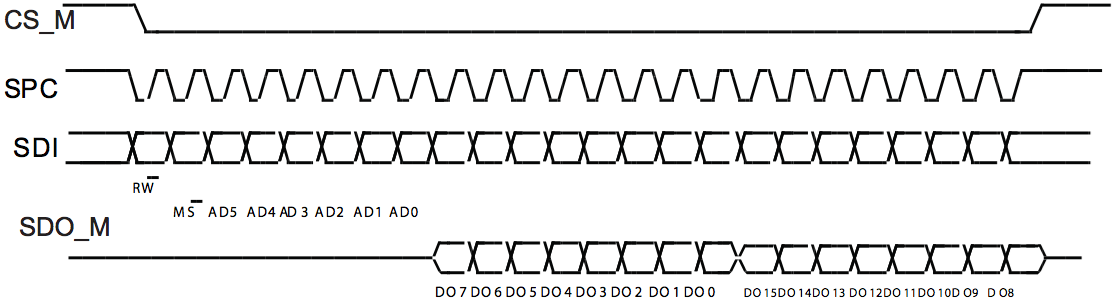
\includegraphics[width=1\textwidth]{multiple_reads.png}}
	\caption{Magnetometer Multiple byte SPI Read Protocol \cite{lsm9ds1}}
	\label{multiple_reads}
\end{figure}

\subsubsection{Register Settings}
The LSM9DS1 IMU requires memory register setting in order to turn on the magnetometer and function properly. The memory register settings are can be set by writing to the IMU in the SPI communication format shown in Figure \ref{magnetometer_spi}. As such, for all of the setting adjustments the $R\overline{W}$ bit is set to 0 signifying a write command.
\par
One register that needs to be written to is the magnetometer's control register 1, or CTRL\textunderscore{}REG\textunderscore{}1\textunderscore{}M, which is at address 20\textsubscript{16}. 7C\textsubscript{16} was written to CTRL\textunderscore{}REG\textunderscore{}1\textunderscore{}M to signify ultra high performance mode for the magnetometer's x- and y-axis, and leave all of the other settings in the register at their defaults \cite{lsm9ds1}.
\par
The other register that needs to be written to is the magnetometer's control register 3, CTRL\textunderscore{}REG\textunderscore{}3\textunderscore{}M, at address 22\textsubscript{16}. 80\textsubscript{16} was written to CTRL\textunderscore{}REG\textunderscore{}3\textunderscore{}M to turn off I\textsuperscript{2}C, turn on the magnetometer in the continuous-conversion mode, and leave all of the other settings in the register at their defaults \cite{lsm9ds1}.
\par
Due to time constraints, we only needed to use the magnetometer. The accelerometer, gyroscope, and barometer were not used so we only needed to set these two registers once.

\subsubsection{Read Registers}
With the magnetometer turned on and its registers set, its data is ready to be read. As such, the $R\overline{W}$ bit is set to 1, and there are two registers that need to be read from in order to ensure data accuracy. 
\par
One register to read from is the status register, STATUS\textunderscore{}REG\textunderscore{}M, which is at address 27\textsubscript{16}. This address is read from until the two least significant data bits read 11\textsubscript{2}, which signifies that new x- and y-axis magnetometer data is ready. Once new x- and y-axis data is ready, the corresponding data registers can be read from \cite{lsm9ds1}.
\par
The x- and y-axis data comes in 16-bit resolution. Due to the SPI transfer protocol shown in Figure \ref{magnetometer_spi}, data is read 8 bits at a time MSB first. Since each axis has 16-bit resolution, each axis has two addresses containing 8-bit data words. Since the x- and y-data addresses are consecutive, we can read 32 bits of data in one cascading read in the format shown in Figure \ref{multiple_reads}. Because of this, we perform a cascading read from address 28\textsubscript{16}, OUT\textunderscore{}X\textunderscore{}L\textunderscore{}M, to obtain the x-axis lower word, the x-axis upper word, the y-axis lower word, and then the y-axis upper word \cite{lsm9ds1}.








\subsection{IMU Implementation}
Since the IMU will be connected to the ZedBoard's Pmod connector, it can be controlled by either the Programmable Logic (PL) or the Programmable Software (PS). Since the IMU's magnetometer data will be used to rotate the rangefinder data according to a compass direction, it will affect the rangefinder's step value. Since the step value is set in the PS, it is easiest to keep all of the IMU's implementation in the PS rather than take advantage of the PS-PL communication setup from Section \ref{sssec:ps_pl}. Another motivation for the PS is that the IMU data processing involves complex trigonometry. Rather than attempt this in the PL, it would be simpler to do in the PS.
\par
The Zynq7 Processing System in the PL needs to be re-customized in order to add SPI capability.

\subsubsection{Re-Customizing the Zynq7 Processing System}
The Zynq7 Processing System is easily re-customizable, as discussed in Section \ref{zynq7processingsystem}. SPI functionality can be added in the processing system's customization window under I/O Peripherals in the MIO Configuration tab. We intend to route the SPI pins to EMIO (Extended MIO) so that we could control one of the ZedBoard's PL Pmod's from the PS. Since both SPI0 and SPI1 have EMIO functionality, we arbitrarily chose SPI0 over SPI1. This process is shown in Figure \ref{enabling_spi0}.

\begin{figure}[H]
	\centerline{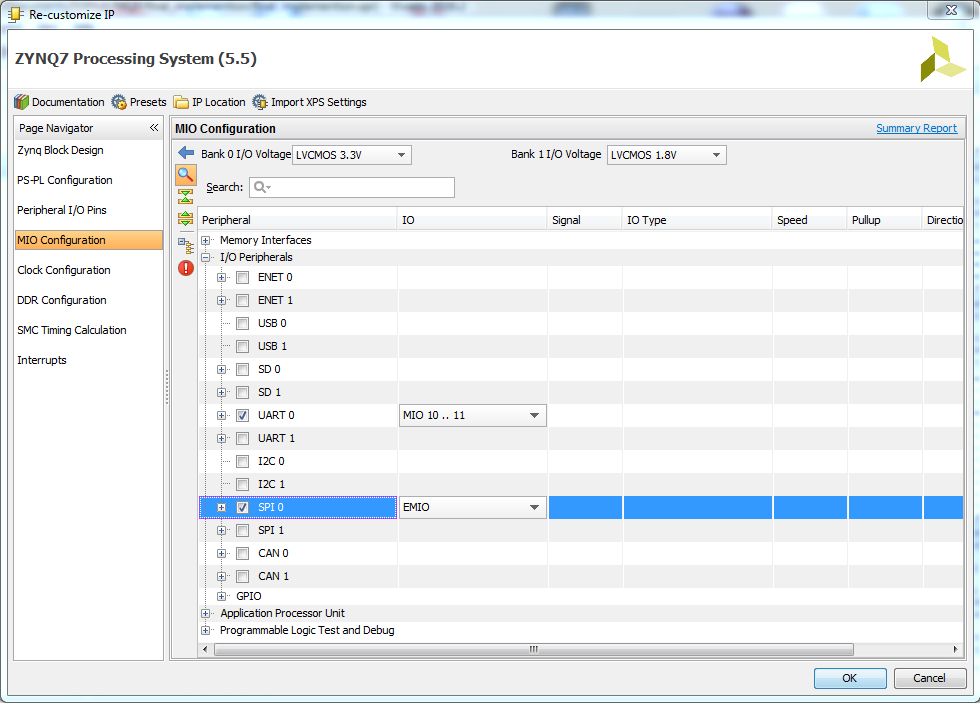
\includegraphics[width=1\textwidth]{enabling_spi0.png}}
	\caption{Re-Customizing the Zynq7 Processing System to Add SPI}
	\label{enabling_spi0}
\end{figure}


\par
talk about rerouting the SPI pins to the EMIO PMOD
\par
ADD NEW SECTION IF THIS ISN'T DONE IN THE PROCESSING SYSTEM CONFIGURATION
\par
This is all you brocahtoa, i got nothing.






\subsection{IMU Data Processing}
The IMU's data processing was implemented in the Programmable Software because it involves complex mathematical equations, and can be easily integrated with the rangefinder's data in the Software Development Kit.

\subsubsection{Programmable Software}
Talk about the math, integration into the rangefinder's code, and how the IMU data rotates the rangefinder's data.

\subsection{Camera Operation}
\subsubsection{Camera Selection}  \label{camdecision}
In order to determine the proper camera modules for this project, several steps needed to be taken. Due to our limited project budget and time constraints, we focused on finding camera modules that were low-cost and simple to communicate with. This ruled out many low-cost camera modules that rely on complicated communications protocols, as well as all commercially available stereo image sensor suites. One other important factor that we sought to satisfy in our camera setup was the use of global shutter cameras, which acquire image data from the entire image sensor at once, rather than sequentially by pixel. The use of global shutter camera modules makes it so that our setup is not susceptible to lens artifacts, or distorted imagery due to moving objects or a moving camera setup. With these factors kept in mind, the decision matrix shown below was created for selecting a proper camera module. Each module evaluated was given a ranking from 1-10, with 10 representing the ideal camera module for our project. 
\par
\singlespacing
\begin{small}
\centerline{
\begin{tabular}{ |L{2cm}|L{1.5cm}|L{2.5cm}|L{1cm}|L{1.7cm}|L{2cm}|L{1.7cm}|L{1.2cm}|L{1cm}| } 
 \hline
 \textbf{Camera Module} & \textbf{Max Frame Rate (FPS)}  & \textbf{Resolution at Max Frame Rate (px.)} & \textbf{Cost} & \textbf{Requires External Adapter} & \textbf{Data Transfer Interface} & \textbf{Shutter} & \textbf{Field of View (deg.)} & \textbf{Rank 1-10}  \\ \hline
 OV7670 & \cellcolor{red!25} 30 & \cellcolor{green!25} 640x480 & \cellcolor{green!50} \$10 & \cellcolor{green!25} No & \cellcolor{green!25} Parallel & \cellcolor{red!25} Rolling & \cellcolor{red!25}  25 & 5  \\ \hline
 Raspberry Pi Camera &\cellcolor{green!25}  90 & \cellcolor{green!25} 640x480 & \cellcolor{green!25}  \$30 & \cellcolor{red!25} Yes, \$53 & \cellcolor{red!25} MIPI (CSI2) & \cellcolor{red!25}  Rolling & \cellcolor{green!25} 49 & 6  \\  \hline
 PC1089K & \cellcolor{green!25} 60 & \cellcolor{green!25} 720x480 & \cellcolor{green!25} \$32 & \cellcolor{green!25} No & \cellcolor{red!50} NSTC/ PAL & \cellcolor{red!25} Rolling & Not Given & 5 \\ \hline 
 OV4682 & \cellcolor{green!50} 330 & \cellcolor{green!25} 640x480 & \cellcolor{red!25} \$89 & \cellcolor{red!25} Yes, \$50 & \cellcolor{red!25} MIPI & \cellcolor{red!25} Rolling & Not Given & 6 \\ \hline
 \textbf{MT9V034} & \cellcolor{green!25} \textbf{60} & \cellcolor{green!25} \textbf{752x480} & \cellcolor{red!25} \textbf{\$73} & \cellcolor{green!25} \textbf{No} & \cellcolor{green!25} \textbf{Parallel} & \cellcolor{green!50} \textbf{Global} & \cellcolor{green!25} \textbf{55} & \textbf{9} \\ \hline   
\end{tabular} }
\end{small}
\vspace{0.5cm}
\doublespacing
\par
Based on our decision matrix, we believed that the MT9V034 camera module would be ideal for our stereo camera interface. These camera modules are the only low-cost global shutter option we were able to find in our research, and are ideal for taking images in a sensor suite that is susceptible to motion. The MT9V034 also uses a parallel data interface and relies on an external clock and shutter trigger, making the module ideal for interfacing with an FPGA-based stereo imaging setup. After obtaining two of the MT9V034 cameras, the operation of the camera modules was then investigated. In order to gather working images from each camera module, we first needed to understand what circuitry our camera module breakouts contained so that we could interface with them. The MT9V034 camera breakouts used have been purchased through Leopard Imaging Inc. Although these camera module breakout boards are intended to be used with Leopard Imaging's LeopardBoard ARM development board, the breakouts were found to contain only the supporting circuitry recommended in the MT9V034 datasheet, and we decided that they would be ideal for our application \cite{livm34lp,mt9v034}. Once the schematics of each camera module breakout were known, it was then possible to design a basic control interface for each camera.
\subsubsection{Camera Signaling}
By default, the MT9V034 camera module will continuously gather image data at 60Hz  as long as it is supplied with an external clock signal and output is enabled \cite{mt9v034}. Several output signals from the camera module are then used to transmit image data. Each image, or frame, is broken up into individual "lines" which correspond to a line of pixels that stretch the width of the frame. Since our camera module captures images at 752x480 pixel resolution, one frame will contain 480 lines of 752 pixels each. The camera module breaks up image data by frame and line, and camera data pins FRAME\_VALID and LINE\_VALID are toggled to indicate the transmission of a frame or line. The timing diagram shown in Figure \ref{FvLv} shows the operation of these pins while transmitting an image.

\begin{figure}[H]
	\centerline{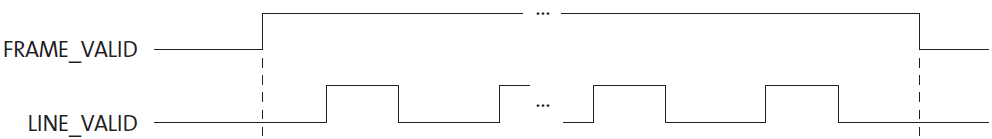
\includegraphics[width=1.0\textwidth]{camFvLv.png}}
	\caption{Frame and Line Valid \cite{mt9v034}}
	\label{FvLv}
\end{figure}

\par
Since the MT9V034 module transmits image data in parallel and each pixel contains 10 bits of resolution, 10 pins are used to transmit pixel values. Pixel data is transmitted in correspondence with LINE\_VALID and output clock signal PIXCLK. When LINE\_VALID is asserted, the pixel data pins are updated with values corresponding to pixels 0-751 of the given line. Values for each pixel are written out on the falling edge of the camera's PIXCLK pin, allowing for each pixel's value to be read on each rising PIXCLK edge. A full LINE\_VALID data transmission sequence will therefore contain 752 PIXCLK cycles, corresponding to the 752 pixels that make up the given line. A timing diagram of this data transmission scheme is shown in Figure \ref{LvDout}.  
\begin{figure}[H]
	\centerline{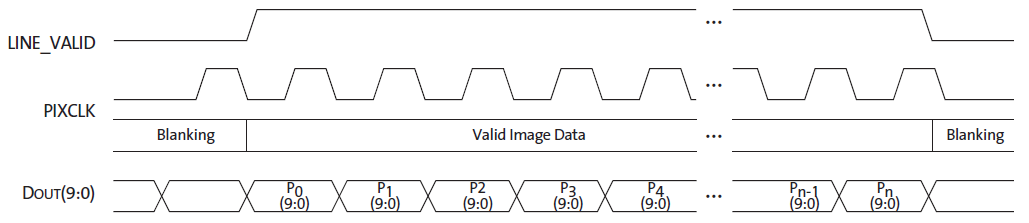
\includegraphics[width=1.0\textwidth]{camLvPckDout.png}}
	\caption{Line Data Transfer \cite{mt9v034}}
	\label{LvDout}
\end{figure}

\par
The default camera data transmission scheme was also examined using an oscilloscope, as shown in Figure \ref{camDataTransfer}, with channels 1-4 corresponding to camera PCLK, FRAME\_VALID, LINE\_VALID, and Data[0], respectively. In the case of Figure \ref{camDataTransfer}, the camera is initially powered off, resulting in an inactive PCLK signal during the beginning of the recording.
\begin{figure}[H]
	\centerline{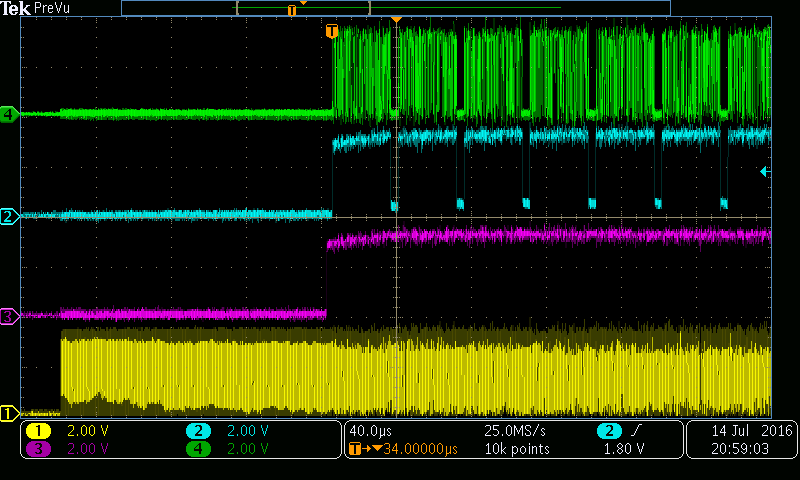
\includegraphics[width=1.0\textwidth]{oScope/pclk_fv_lv_data2/tek00004.png}}
	\caption{Camera Data Transfer}
	\label{camDataTransfer}
\end{figure}

\subsubsection{I$^2$C Control} \label{cameraI2Cdescription}
The MT9V034 Camera module's mode of operation can be configured using a standard I$^2$C control interface. I$^2$C, or Inter-Integrated Circuit, is a bidirectional serial interface that allows for a master device to read from and write to several slave devices sharing the same data bus. An I$^2$C interface will use a Serial Data Line (SDA) and Serial Clock Line (SCL) that are normally pulled to 5V. When one connected I$^2$C device wishes to communicate with another, it will pull the SDA line low while leaving the SCL line high. The master device will then begin clocking the SCL line, and SDA will be used to transfer 7 bits representing the address of the desired slave device, along with an 8th bit representing whether it would like to read from or write to the device. An example of this transfer is shown in Figure \ref{I2Cexample}. A second 8 bit sequence representing a specific register within the slave device may also be transmitted following the device address. For example, if the master device wishes to write to slave device 0x40 at register 0x00, it will transmit 0x41 (address 0x40 and WRITE), followed by 0x00. If the slave device receives this transmission, it will acknowledge by pulling the SDA line low. At this point, the master can then transmit the value that it wishes to write to the given slave address and register. If the operation were a read rather than a write, the slave would transmit a value back to the master.  
\par
\begin{figure}[H]
	\centerline{
\includegraphics[width=1.0\textwidth]{I2C_data_transfer.png}}
	\caption{Example I$^2$C Data Transfer}
	\label{I2Cexample}
\end{figure}

Based on the LIVM34LP camera board schematic, each breakout board have been configured so that its camera is accessible at I$^2$C address 0x58 \cite{livm34lp,mt9v034}. Note that since both cameras come configured with the same I$^2$C bus address, a pullup resistor must be added to one of the cameras I$^2$C address lines so that both are individually accessible on a shared bus.

\subsubsection{Image Buffering}
Since each camera image contains 752x480 pixels with 10 bits of resolution per pixel, a full camera image will consume 3,609,600 bits, or 440.6kB, as shown in Equation \ref{imagesize}.
\begin{equation} \label{imagesize}
Image\,\,Size = 752px*480px*10\frac{bits}{pixel} = 3609600\,bits*\frac{1\,byte}{8\,bits}*\frac{1 kB}{1024\,bytes} = 440.625kB
\end{equation}
\par
In order to send a camera image to a computer or monitor for viewing, several steps need to be taken. Although it would be ideal to transfer the image directly from the camera to a computer or display, this would be difficult to achieve due to the high speeds of the camera's data output. In order to properly synchronize camera data with a VGA display, both the camera and VGA display would have to run at exactly the same clock speed, and would need to have the same amount of vertical and horizontal blanking to display each pixel in its correct location. If the image were transferred to a computer, the act of packaging the information so that it may be interpreted by said computer would place severe limitations on the speed of the system. A proper solution to these timing issues would be to buffer the image between the camera and the desired output source, since this would allow for separate clock domains to be used for camera data transfer and data output. However, the act of locally buffering a camera image on an FPGA would also be difficult due to low memory resources. 
\par
Although 440kB may seem like a relatively small image size, creating a buffer object large enough for storing said image would consume an extremely large amount of logic. For reference, a standard Nexys3 FPGA evaluation board contains only 18kB of onboard Block RAM (internal memory), and would not be able to buffer an image of this size without the use of external memory\footnote{Xilinx, \textit{Spartan-6 FPGA Block RAM Resources}, 11.\\  \url{http://www.xilinx.com/support/documentation/user_guides/ug383.pdf}}. This leaves the final option of using either external memory or a First-In First-Out (FIFO) memory array for transferring a captured image between clock domains. During initial development, an AL422B FIFO IC was used, since the IC has been created specifically for buffering VGA imagery similar to that of the MT9V034 camera module, and can be connected directly to the camera module outputs \cite{al422b}. The AL422B FIFO module contains 3M-bits of RAM that can be written to and read from in parallel, and supports separate input and output clock speeds between 1-50MHz \cite{al422b}. This means that the camera module can write pixel data to the FIFO as long as it operates at a speed between 1 and 50MHz, and the FPGA can independently read from the FIFO at any speed within the same range. Note that since this FIFO supports only 8-bit parallel data in and out, the lowest two bits of camera pixel data must be truncated. This isn't a major issue, since the truncation will correspond to a 4/1024 reduction in the range of values that each pixel can map to.
\subsection{Disparity Algorithm}
Some important properties of the stereo camera setup used in this project may be taken advantage of in order to extract 3D depth information from 2D image data. Since both cameras will capture imagery of the same scene from slightly different vantage points, depth information on the scene may be extracted by calculating the pixel offsets, or disparity, between the same object's relative location in each image. Given this pixel offset, one may determine the distance from the camera pair to a given object using simple geometry based on the focal length and baseline of the stereo camera pair. Note that each camera must have the same focal length, or distance from the image sensor to the lens of the camera. The baseline of the stereo camera pair is the distance between the two image sensors, which is usually a similar length to the average distance between a pair of human eyes  \cite{collins}. 
\subsubsection{Image Rectification} \label{rectsec}One simple way of determining the disparity between objects in a stereo image pair is known as the Sum of Absolute Differences. The Sum of Absolute Differences algorithm operates under the assumption that objects in both camera images lie on the same horizontal line between both images, known as an epipolar line. An example of shared epipolar lines between camera imagery is shown in Figure \ref{epipolarLines} below. Although an ideal stereo camera setup would contain shared epipolar lines between camera images, raw image data from each camera will contain slight differences in object location based on the physical position of the camera modules, as well as minor differences in the lenses of each camera. Both input images can be adjusted to share the same epipolar lines through a post-processing step known as image rectification. 
\par
\begin{figure}[H]
	\centerline{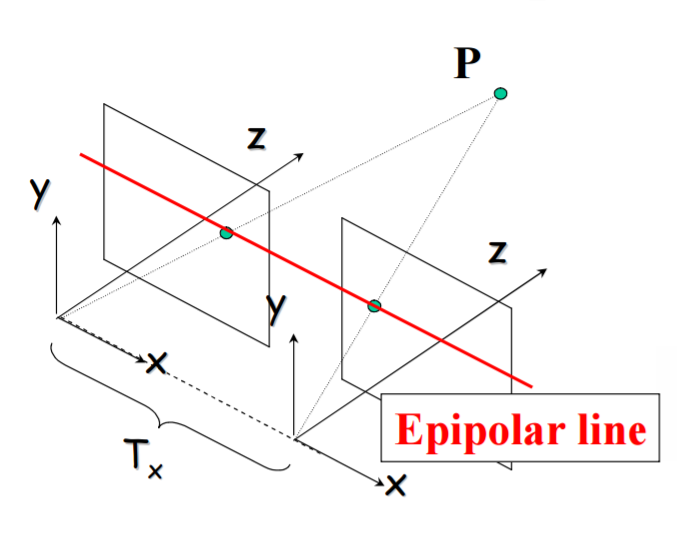
\includegraphics[width=0.5\textwidth]{epipolarLines.PNG}}
	\caption{Horizontal Epipolar Lines \cite{collins}}
	\label{epipolarLines}
\end{figure}
\par
A pictorial representation of the process of stereo image rectification is shown in Figure \ref{rectification} below \cite{mattoccia_slides}. This process is achieved using a 3x3 matrix coordinate transform based on parameters obtained from the external calibration process. 
\begin{figure}[H]
	\centerline{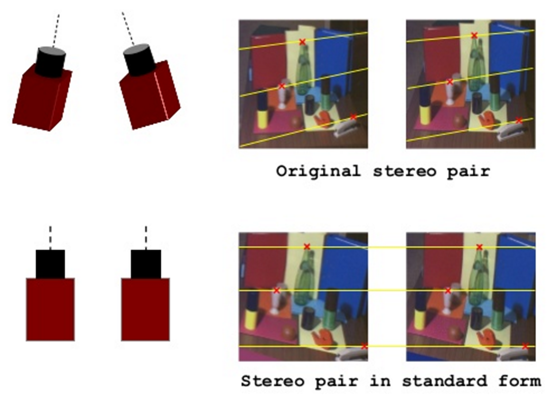
\includegraphics[width=0.5\textwidth]{rectification.png}}
	\caption{Stereo Image Rectification \cite{mattoccia_slides}}
	\label{rectification}
\end{figure}
\par
After a given pair of images has been rectified, it is then possible to perform the Sum of Absolute Differences on the given image pair in order to extract depth information. 
\subsubsection{Sum of Absolute Differences} \label{SADexample}
The method used in our disparity algorithm implementation is known as the Sum of Absolute Differences, or SAD. SAD is a common digital image processing technique used to measure the similarity between blocks of image data. In the case of our stereo camera interface, a SAD algorithm is used to search along epioplar lines in the right image for pixel blocks that match a template block selected from the left camera image. This process is performed using 7x7 pixel search blocks over 20 pixel horizontal ranges, and is repeated throughout the image. The expression for the sum of absolute differences is shown in Equation \ref{disparityEQN} below. 
\par
% sum(sum(abs(template-block)))
\begin{equation}\label{disparityEQN}
SAD = \sum_{x}^{}\sum_{y}^{}|template-block|
\end{equation}
\par
A visual representation of the Sum of Absolute differences is shown in Figure \ref{SAD}, with the top image showing the left image template block, and the middle image showing the right image search window in relation to the location of the template block. Below both images is a visual representation of the Sum of Absolute Differences between the template block and the current search block, outlined in white. In the case of the current search, the template and search blocks are relatively different, resulting in a high SAD value. 
\par
\begin{figure}[h]
	\centerline{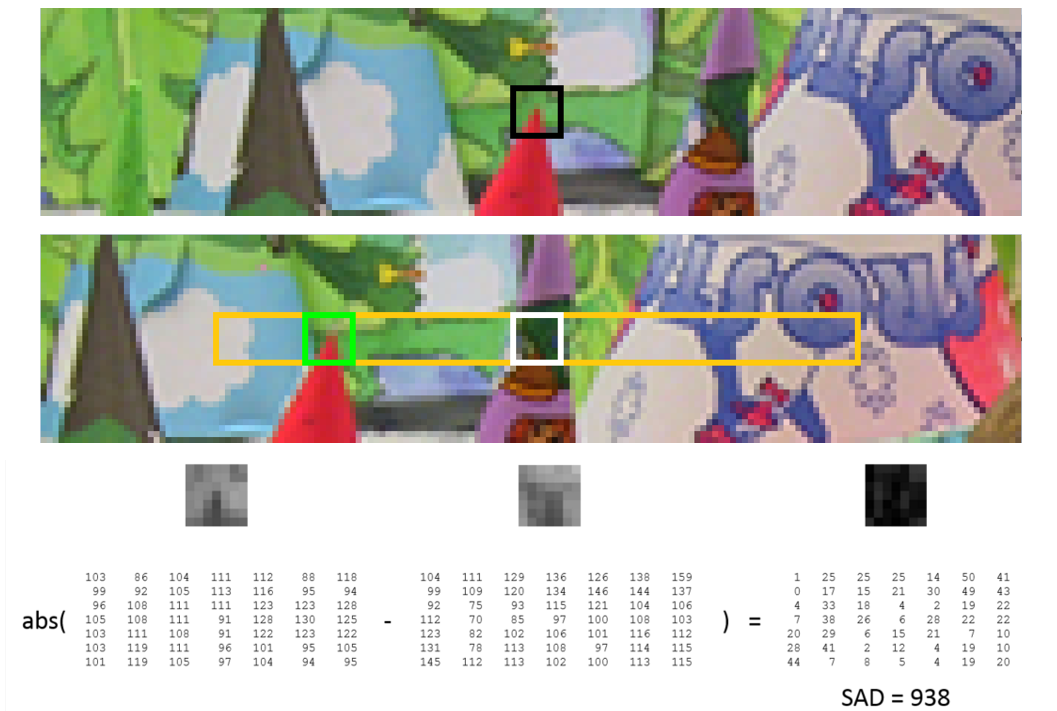
\includegraphics[width=0.75\textwidth]{SAD.PNG}}
	\caption{Sum of Absolute Differences \cite{mccormick}}
	\label{SAD}
\end{figure}
\par
Since the disparity algorithm used in this implementation calculates the sum of absolute differences for multiple search blocks, the resulting SAD values for each search block can be compared to find the location of the most similar matching block in the search image. Due to the nature of the SAD algorithm, lower SAD values indicate higher similarity between the template and search blocks. This comparison is demonstrated in Figure \ref{blockMatching} below. In the case of Figure 
\ref{blockMatching}, higher match score values for each search block indicate lower SAD values.
\par
\begin{figure}[h]
	\centerline{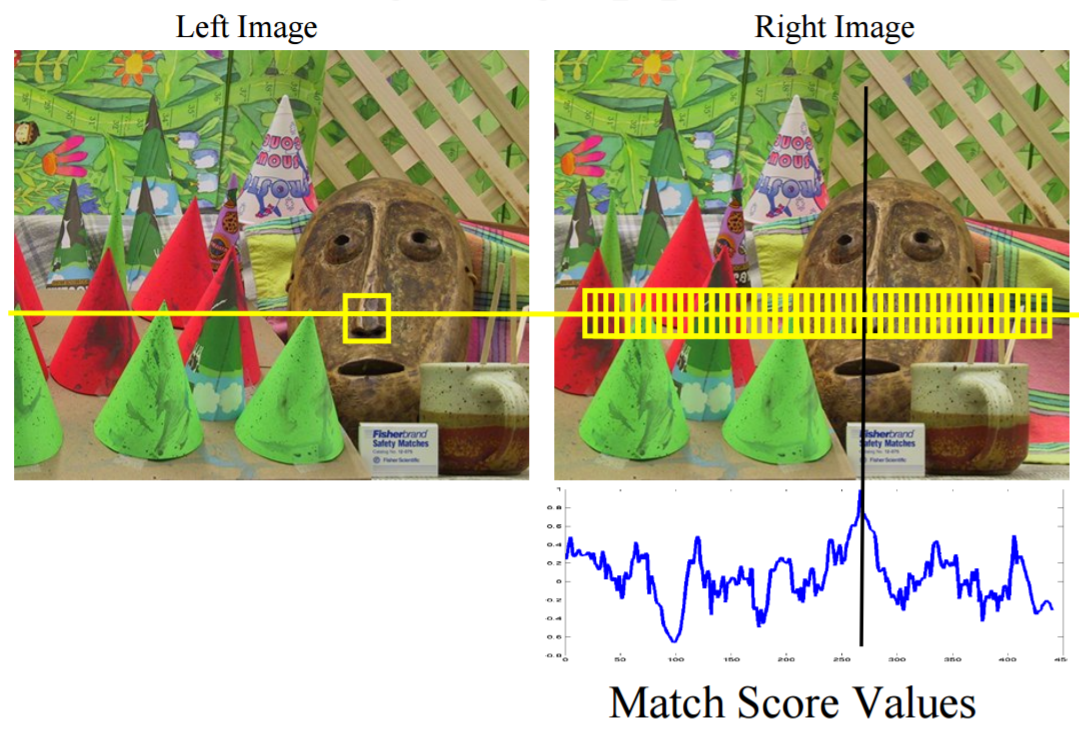
\includegraphics[width=0.75\textwidth]{blockMatching.PNG}}
	\caption{Block Matching Overview \cite{collins}}
	\label{blockMatching}
\end{figure}
\par
The SAD at multiple search points can be used to estimate the pixel offset between the template block and matching search block based on array index locations, since all SAD values for a single search are stored in a vector. This pixel offset is known as the disparity value for a given template and search block. The disparity $d$ at a given point can be transformed into a unit of distance using the focal point $f$ and baseline distance $T_x$ between image sensors as shown in Equation \ref{disp2dist} below. 
\par
\begin{equation}\label{disp2dist}
depth = Z = \frac{fT_x}{d}
\end{equation}
\par
Pixel coloration values in a disparity image are based on the distance calculation shown in Equation \ref{disp2dist}, where each pixel is referenced to the disparity at a given template block's location. An example disparity image created using a given pair of test images is shown in Figure \ref{disparityOutput} below. 
\par
\begin{figure}[H]
	\centerline{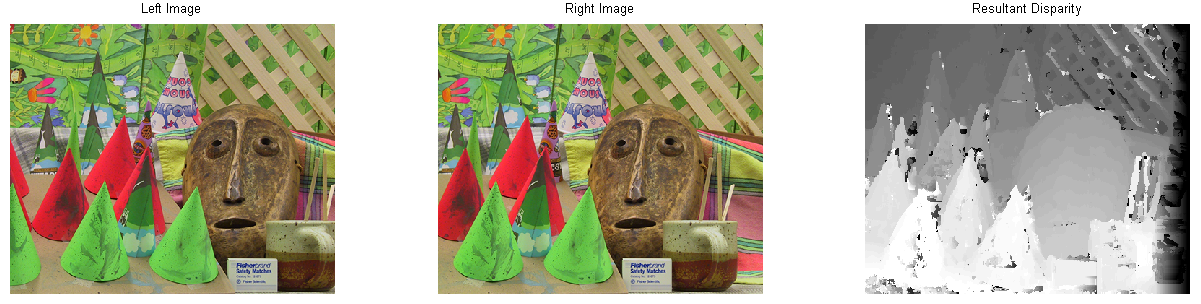
\includegraphics[width=1.1\textwidth]{disparity.png}}
	\caption{Disparity Algorithm Output}
	\label{disparityOutput}
\end{figure}
\subsection{Combined Implementation}
The following sections describe the integration of each individual sensor's data into the final, combined implementation. The rangefinder and disparity data was combined to produce accurate depth estimations. This data was also integrated with navigational data to create a more accurate approximation of the sensor suite's relative surroundings. 

\subsubsection{Rangefinder and Disparity Data Integration}
3D depth information from the disparity algorithm was combined with 2D depth information from the scanning laser rangefinder in order to increase the overall accuracy of the system. Since the rangefinder and stereo camera interface shared a horizontal viewing plane and both sensors gathered information on the same scene, there was some distinguishable overlap in sensor data. This overlap was taken advantage of in order to produce a more accurate 2D "floorplan" of the area being observed. This type of data integration is especially useful in situations where the scanning laser rangefinder is out of range.
\par
Through the use of a moving average Finite Impulse Response (FIR) filter across a horizontal line of depth information from the disparity algorithm output, a single line of depth information obtained was correlated with rangefinder data obtained from the same scene. Note that although 2D rangefinder data is organized using a polar coordinate scheme, the output buffer used for displaying rangefinder data via VGA contains the same data in a Cartesian format. This Cartesian rangefinder data was easily combined with averaged disparity depth information at the output stage, where both sensors' data is displayed relative to the same central location on screen. 
\par
In order to correlate both sensors' data for a combined output mode, the field of view of each device was taken into account. Since each camera has an approximate 55$^\circ$ field of view, and camera imagery is 752 pixels wide, the stereo camera interface has a deg:pixel ratio of $\frac{752}{55}=13.67\frac{px}{deg}$. Output data from the rangefinder is divided into 768 steps over a 270$^\circ$ field of view. In order to correlate disparity data with rangefinder data, the averaged disparity depth line was converted an equivalent number of "steps" worth of data. The conversion factor for pixels of disparity depth to "steps" was calculated as shown by Equation \ref{yeeboi}.
\begin{equation} \label{yeeboi}
13.67\frac{px}{deg}*\frac{270^\circ}{768\,\,steps} = 4.8\frac{px}{step}
\end{equation}
\par
The output from the disparity pixel line was scaled down by an approximate factor of 4.8 in order for it to correlate with depth information from the scanning laser rangefinder. Once this scaling process was complete, depth information from the disparity algorithm was directly overlaid on the 2D scanning laser rangefinder's output in order to produce a combined depth map. 

\subsubsection{Accounting for Navigational Data}
With the IMU's accelerometer, gyroscope, and magnetometer, displacement and orientation was calculated. The orientation and displacement was displayed on a screen to show the device's behavior and its location. This was combined with the rangefinder's data to show the orientation of the device, where it has traversed, and the distance away of the objects closest to it.
\par
The IMU's compass data was combined with the rangefinder's step count. Changing the step count rotates the distance data around the device by changing the starting point of the data processing. This changes the direction of the rangefinder's $240^\circ$ field of vision. For example, an IMU reading corresponding to due West is a rotation of $90^\circ$ counterclockwise from due North. By Equation \ref{StepsPerDegree}, $90^\circ$ equates to 256 rangefinder steps. So, the rangefinder's data essentially begins at step 256 and end at step 1024 or 0\footnote{step 768 + 256 step offset = 1024. Since there are 1024 rangefinder steps in a circle, step 1024 is the same as step 0.}, seen in Figure \ref{rangefinder_fov}.

\begin{equation}
	90^\circ \div \dfrac{360^\circ}{1024 \textrm{ } steps}  = 256 \textrm{ } steps
	\label{StepsPerDegree}
\end{equation}

\par
Due to time constraints, the IMU displacement data was not able to be incorporated into this project. The displacement data was planned to change the device's location on the VGA screen. Ideally, the device would appear to traverse the screen as the device itself traverses a location, with the rangefinder's data traveling with it. Since the rangefinder's data is stored in such a way that it is localized to the device's location, incorporating the IMU's displacement data is as easy as obtaining the data from the IMU in the PS and sending it to the PL via an extra PL read register discussed in Section \ref{sssec:creatingCustomIP}.




\newpage 
\section{Testing and Results}
After learning how to interface with the chosen sensors, it was then possible to begin creating test implementations for each individual sensor. Many of the initial tests performed on each sensor were designed so that they could be later integrated into a final design, as detailed in the following sections. 
\subsection{Rangefinder Testing}
The URG-04LX scanning laser rangefinder requires an external 5V power source connection. With the power connected and the device on, the device is ready and waiting for communication.

\subsubsection{Testing via the Data Viewing Tool}
The URG-04LX has a data viewing tool which is a useful application by Hokuyo Automatic Co. that can be used to view, record, and replay the device's data. To use this tool the device was plugged into a computer via its USB port. Figure \ref{URGBenriStandard_pic} below shows a screen capture of the application recording data captured by the rangefinder.

\begin{figure}[H]
	\centerline{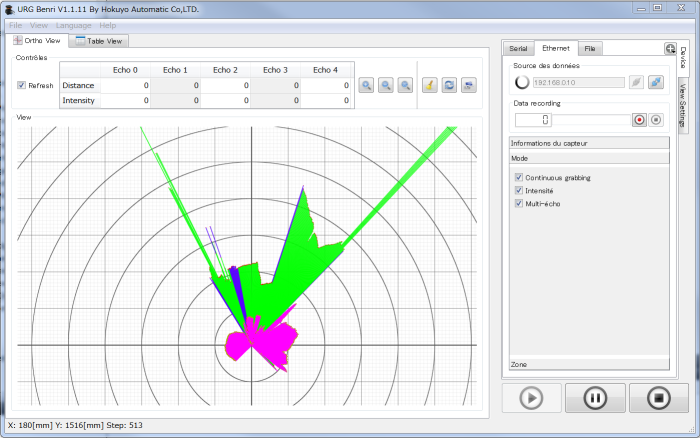
\includegraphics[width=1\textwidth]{UrgBenri_screenshot.png}}
	\caption{Screen Capture of the URG-04LX Data Viewing Tool \cite{URGBenriStandard_ref}}
	\label{URGBenriStandard_pic}
\end{figure}

Note that the start point of 0, end point of 768, and dead zone align to that shown in Figure \ref{rangefinder_fov}. For this project the data viewing tool was used to verify our project's data processing functionality.

\subsubsection{Command Testing}
In addition to the data viewing tool, the rangefinder's commands were tested by connecting it to a laptop via its USB port. We used PuTTy, a serial console application, to communicate with the rangefinder. Figure \ref{rangefinder_putty} shows the data transfer via PuTTy between a laptop and the rangefinder. Note that PuTTy only shows data received, and that the rangefinder always echoes back the command that it receives.

\begin{figure}[H]
	\centerline{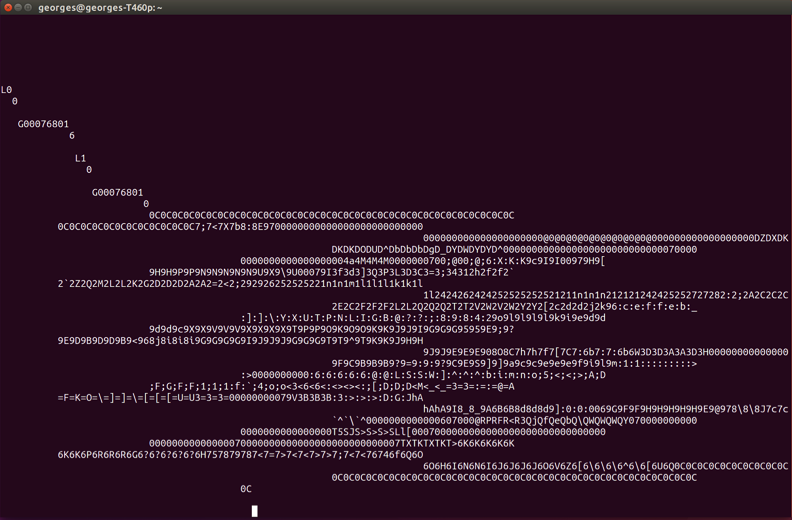
\includegraphics[width=1\textwidth]{rangefinder_putty.png}}
	\caption{Rangefinder Communication Test via PuTTy}
	\label{rangefinder_putty}
\end{figure}

The figure above shows four communication sequences. The first is the laser illumination command 'L0\textbackslash{}n'. Since the laser defaults on, this command turned the laser off. The rangefinder responded to this command first with the echo 'L0\textbackslash{}n', and then with '0', indicating success. The second command is our data acquisition command 'G00076801\textbackslash{}n'. The rangefinder responded with '6', indicating an error code, which was caused by the laser being off. The third command is the laser illumination command again, which turns on the laser. The rangefinder's response was '0' again, indicating success. The last command shown is the data acquisition command again. The rangefinder's response begins with '0', indicating success, followed by the distance data block. The data block consists of 768 points, specified by the data acquisition command. Each data point consists of two characters \cite{urg04lx_datasheet}. By communicating with the rangefinder via PuTTy, we were able to observe the rangefinder's behavior and confirm the data acquisition command functions properly. This testing also verified that communication via the rangefinder's USB port was working.

\subsubsection{Communication via USB On-The-Go (OTG)}
With communication via the rangefinder's USB port working, we decided to continue with this mode of communication. The ZedBoard supports USB On-The-Go (OTG) which is a specification that allows USB devices to act as a host for other USB devices \cite{usb-otg}. With USB OTG, a device chooses to act as a peripheral or a host if necessary. For the purpose of this project, the ZedBoard should act as the host by initiating communication with the rangefinder. Enabling USB OTG can be done in the Zynq7 Processing System and controlled through the PS. The rangefinder's laser illumination command was chosen to be transmitted from the ZedBoard to test the communication. This command was chosen because when received, the status LED on the rangefinder blinks until the laser is turned back on, which is a simple way of verifying successful communication. In addition, when a command is transmitted via UART from the ZedBoard, its TX LED flashes. A fully successful transaction observes the ZedBoard's TX LED flashing and then the status LED on the rangefinder blinking.
\par
The ZedBoard was programmed, the rangefinder was turned on, and the two devices were connected by a standard micro-USB to mini-USB cable. The ZedBoard transmitted the command, as signified by the blink of the TX LED. However the rangefinder did not acknowledge the command; its status LED stayed lit signifying the laser was on. Due to this failure\footnote{This communication failure was most likely due to the lack of necessary hardware, as USB OTG requires an adapter that controls which device will be hosting the communication. Without this adapter, both USB devices act as a peripheral, and neither will initiate communication \cite{usb-otg}.}, using USB OTG was not implemented. Instead the methodology described in Section \ref{sssec:rangefinder_communication} was implemented.

\subsubsection{Communication via Pmod}
Once we decided not to continue with USB OTG, we routed the UART signals to a Pmod connector, described in Section \ref{sssec:rangefinder_communication}. To make sure that UART via Pmod was functioning correctly, the transmit pin was measured with an oscilloscope. The laser illumination command "L0\textbackslash{}n" was transmitted and observed indicating success, as shown in Figure \ref{laser_illumination}. Note that this is a TTL signal.

\begin{figure}[H]
	\centerline{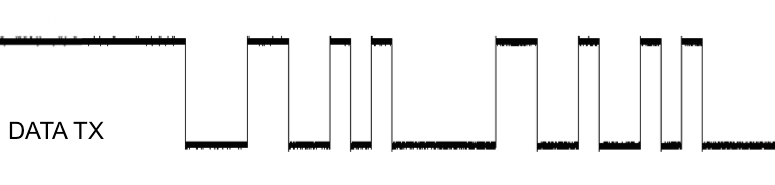
\includegraphics[width=.7\textwidth]{laser_illumination_labeled.png}}
	\caption{Laser Illumination Command TTL Oscillogram}
	\label{laser_illumination}
\end{figure}

The RS-232 to TTL converter with the attached breakout board was attached to the ZedBoard. The converter's V\textsubscript{CC} and GND were connected to the ZedBoard Pmod's respective V\textsubscript{CC} and ground pins. When these pins were connected, the converter's power LED turned on. In addition, the converter's RX and TX pins were connected to the ZedBoard's respective TX and RX pins. The breakout board's TX pin was measured on the oscilloscope to observe the resultant RS-232 waveform. However when the command was transmitted from the ZedBoard, there was no change on the oscilloscope. We disconnected the converter's TX and RX pins and reconnected them such that the converter's RX and TX pins were connected to the ZedBoard's respective RX and TX pins. The laser illumination command was re-transmitted and the waveform in Figure \ref{rangefinder_rs232} was observed on the oscilloscope. The oscillogram shows a waveform from +6V to -6V, which is a valid RS-232 signal.

\begin{figure}[H]
	\centerline{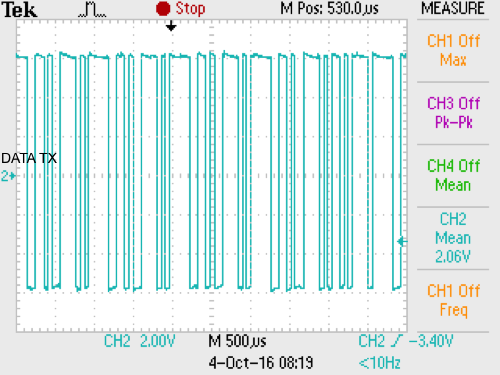
\includegraphics[width=.7\textwidth]{rangefinder_rs232_label.png}}
	\caption{Laser Illumination Command RS-232 Oscillogram}
	\label{rangefinder_rs232}
\end{figure}

With the communication functioning properly, the rangefinder's RX and TX were connected to the breakout board's respective TX and RX pins, and the laser illumination command was transmitted from the ZedBoard. The rangefinder's status LED started blinking, signifying that it received the laser illumination command and the laser was turned off. This test's success indicated that the rangefinder's communication was completely successful.

\subsubsection{PS-PL Testing}
Once UART communication was verified, the next step was to test the PS-PL communication. In order to test the communication, UART was reconfigured in the processing system to be routed to USB UART.
\par
PL to PS communication was tested first, by using a PL button press to initiate a UART transfer. With UART routed to USB UART, the TX LED will flash when data is transmitted. In the PL, BTNR was used as an input and was wired into the AXI's output register, $reg\textunderscore{}data\textunderscore{}out$, as $slv\textunderscore{}reg0$, as seen on line 368 of the custom IP's instantiated file located in Appendix \ref{customIPaxi}. In the PS, the data was read from the AXI bus by pointing to the address in memory where the PL's output register, $slv\textunderscore{}reg0$, is located. This address was found in the SDK in the $system.dhf$ file, which contains the hardware platform specifications. The base address is the cell with the same name as the custom IP. For this project, the base address was 43C00000\textsubscript{16}. Since $slv\textunderscore{}reg0$, the first of the four designated memory registers, was used there does not need to be any address offset. Reading from the PL was implemented on line 30 of the PS, shown in Appendix \ref{ps_code}, by using Xilinx's function $Xil\textunderscore{}In32$ to read the data from the memory address that is $baseaddr\textunderscore{}p$\footnote{This could also have been accomplished by using a pointer to read the data from the memory address that is $baseaddr\textunderscore{}p$.}. Once the setup was complete, the ZedBoard was programmed and connected to a serial console. BTNR was pressed and the TX LED lit up, indicating that PL to PS communication was functioning properly.
\par
PS to PL communication was tested next per use of the VGA screen. For this test, the PS receives the transmit signal from the PL and then waits for 768 data points to be received, just as if the rangefinder were connected. Since UART was routed to USB UART, the ZedBoard communicated with a serial console. Through the serial console, rangefinder communication was simulated by inputting a block of rangefinder data. The data was written to the PL one data point at a time by writing to $slv\textunderscore{}reg1$, as on line 239 of the custom IP's instantiated file located in Appendix \ref{customIPaxi}. This register is located one memory register from the base address of the custom IP because it is the second of the four designated memory registers. The function $Xil\textunderscore{}Out32$ was first tested but no results were observed, so a pointer was used to write to the base address offset by one memory register. This is seen on line 198 of the PS, in Appendix \ref{ps_code}. The data written to $slv\textunderscore{}reg1$ was the distance data point, a data valid flag, and the rangefinder step. These were manipulated to fit into one 32-bit integer by shifting each to a unique bit location of a buffer, $data\textunderscore{}enable\textunderscore{}step$.
\par
To test data accuracy in addition to PS to PL communication, the block of data sent from the serial console was constant. With data constant across all steps of the rangefinder's field of view, $270^\circ$ of a circle are intended to be drawn around the rangefinder on the VGA screen. With the VGA module set up and the rangefinder data processing ready to be tested, the ZedBoard was programmed. When BTNR was pushed, an image similar to Figure \ref{badCircle} was observed on the VGA screen with the red dot being the device and the black lines being the rangefinder's distance data.

\begin{figure}[H]
	\centerline{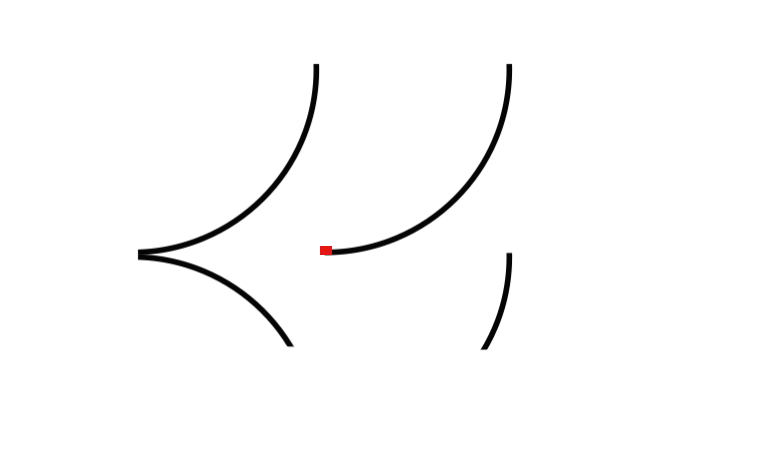
\includegraphics[width=.5\textwidth]{badCircle.png}}
	\caption{PS to PL Communication Test with Constant Data}
	\label{badCircle}
\end{figure}

Although a circle was not observed, this test confirmed the PS to PL communication was functioning properly. The shape appears to look like four quadrants of a circle in the wrong direction. Since the lines seem semi-circular, the polar-to-rectangular transformation were successful, too. The problem was a minor sign issue with the rangefinder's data processing in the PL. The signs in each necessary quadrant were fixed and the test was repeated with Figure \ref{goodCircle} observed on the VGA screen.

\begin{figure}[H]
	\centerline{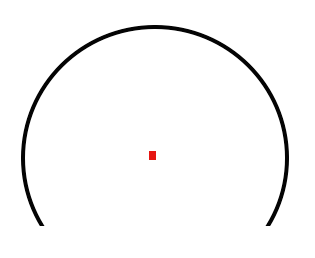
\includegraphics[width=.4\textwidth]{goodCircle.png}}
	\caption{PS to PL Communication with Constant Data and Edited Data Processing}
	\label{goodCircle}
\end{figure}

With the PS-PL communication and rangefinder data processing functioning perfectly, the rangefinder itself was attached and tested.

\subsubsection{Data Testing}
UART was re-routed to the PS Pmod in order to test the entire rangefinder implementation. The rangefinder was powered by the lab bench power supply and was connected on the RS-232 breakout side of the RS-232 to TTL converter, with the ZedBoard connected to the TTL side. The ZedBoard was connected to the VGA screen, and then was programmed. BTNR was pushed to initiate the UART transfer and Figure \ref{first} shows the VGA output.

\begin{figure}[H]
	\centerline{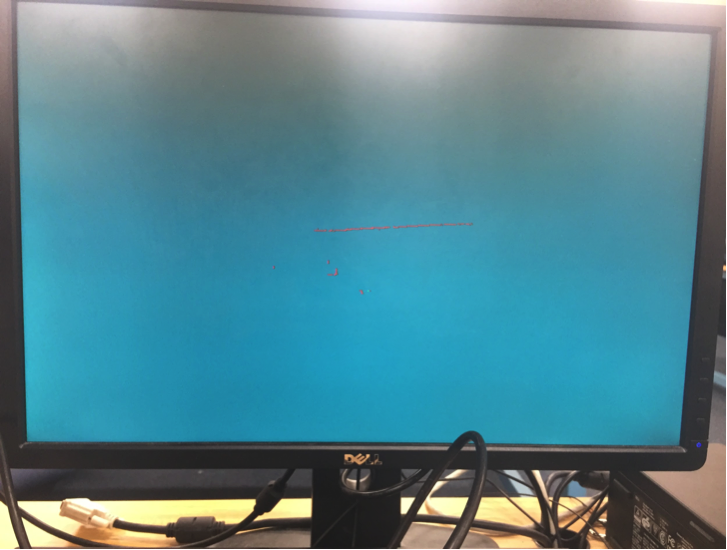
\includegraphics[width=.7\textwidth]{first.png}}
	\caption{Rangefinder Data Observed on VGA Screen}
	\label{first}
\end{figure}

Next BTNR was pushed again to start another data transfer, but there was no observed functionality. The button was held down until the subsequent data transfers in Figure \ref{subsequent} were observed on the VGA screen.

\begin{figure}[H]
	\centerline{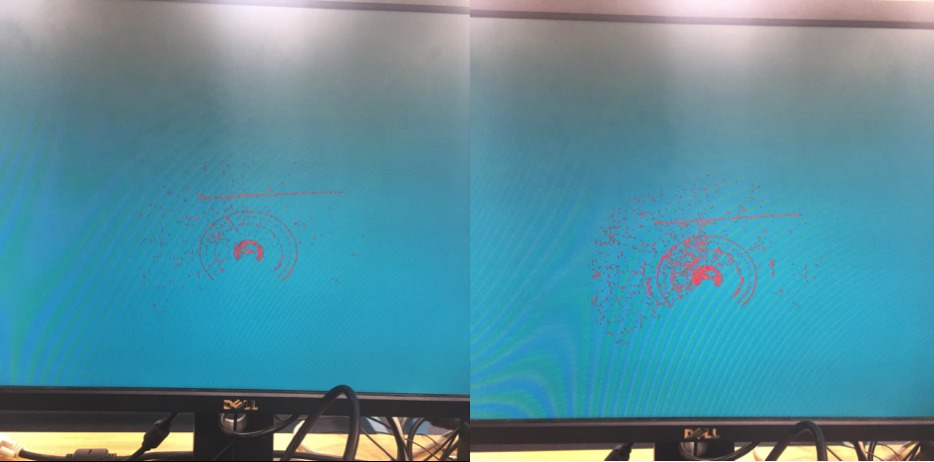
\includegraphics[width=.9\textwidth]{subsequent.jpg}}
	\caption{Subsequent Rangefinder Data Observed on VGA Screen}
	\label{subsequent}
\end{figure}

In the SDK the PS was not accounting for enough data points. When the rangefinder receives a command from the ZedBoard it echoes back the command. This is used as a test to ensure data accuracy. Since not enough data was being accounted for, the extra data was writing into the next data transfer's input echo buffer. As a result, the echo received from the rangefinder did not match the command transmitted and the rest of the data was garbage. The PS was edited to account for all of the data points and the data transfers were able to be triggered every time BTNR was pressed.
\par
Figure \ref{labtest1} shows a test of the rangefinder where its output was compared to the objects around it.

\begin{figure}[H] 
	\begin{subfigure}{1\textwidth}
	\centering
		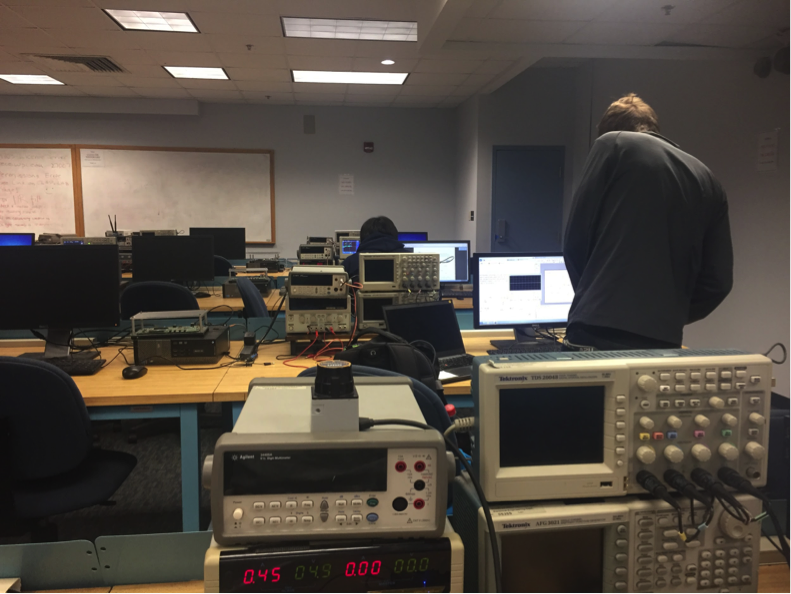
\includegraphics[width=0.75\linewidth]{labtest1_1.png}
		\caption{Lab at WPI}
		\label{lab1}
	\end{subfigure}
	\begin{subfigure}{1\textwidth}
	\centering
		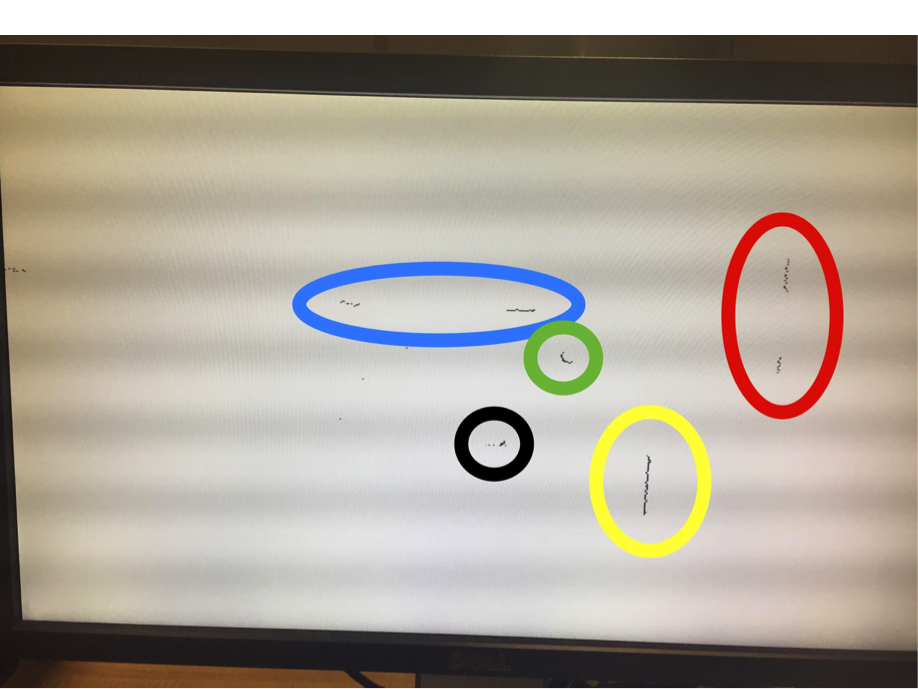
\includegraphics[width=0.75\linewidth]{labtest1_2.png}
		\caption{2D Rangefinder "Floorplan" of Lab at WPI}
		\label{floorplan1}
	\end{subfigure}
	\caption{First Lab Test of Rangefinder Functionality}
	\label{labtest1}
\end{figure}

In Figure \ref{labtest1}(\subref{floorplan1}), the data points in the black circle represent the rangefinder and the lab bench oscilloscope that is right next to it. The straight line circled in yellow is the wall directly to the right of the lab bench. The lines circled in red show the lab doorway with the door open. The data in the green circle is the student in Figure \ref{labtest1}(\subref{lab1}), and the lines in blue are the oscilloscopes and computers in front of the rangefinder.
\par
Next, the screen was cleared, the rangefinder was rotated $180^\circ$, and the process was repeated.

\begin{figure}[H] 
	\begin{subfigure}{1\textwidth}
	\centering
		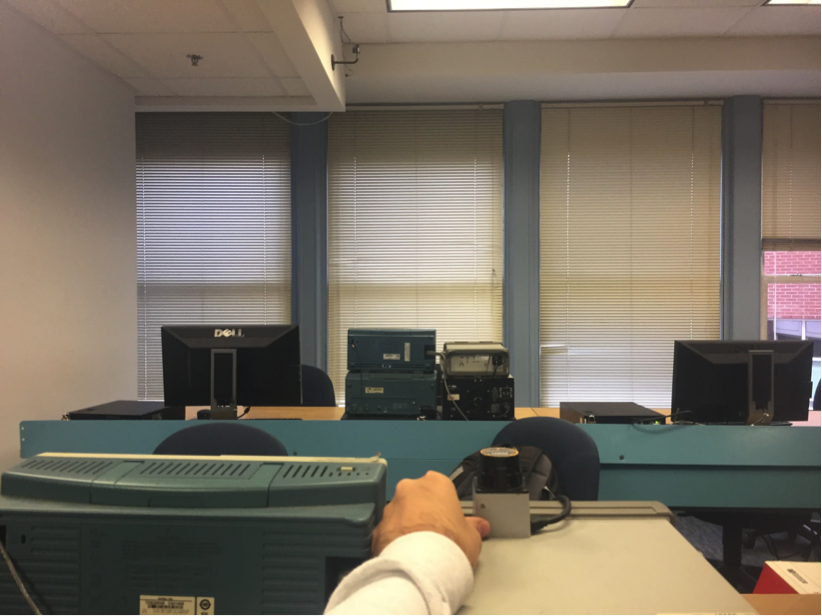
\includegraphics[width=0.75\linewidth]{labtest2_1.png}
		\caption{Lab at WPI with $180^\circ$ Change of Orientation}
		\label{lab2}
	\end{subfigure}
	\begin{subfigure}{1\textwidth}
	\centering
		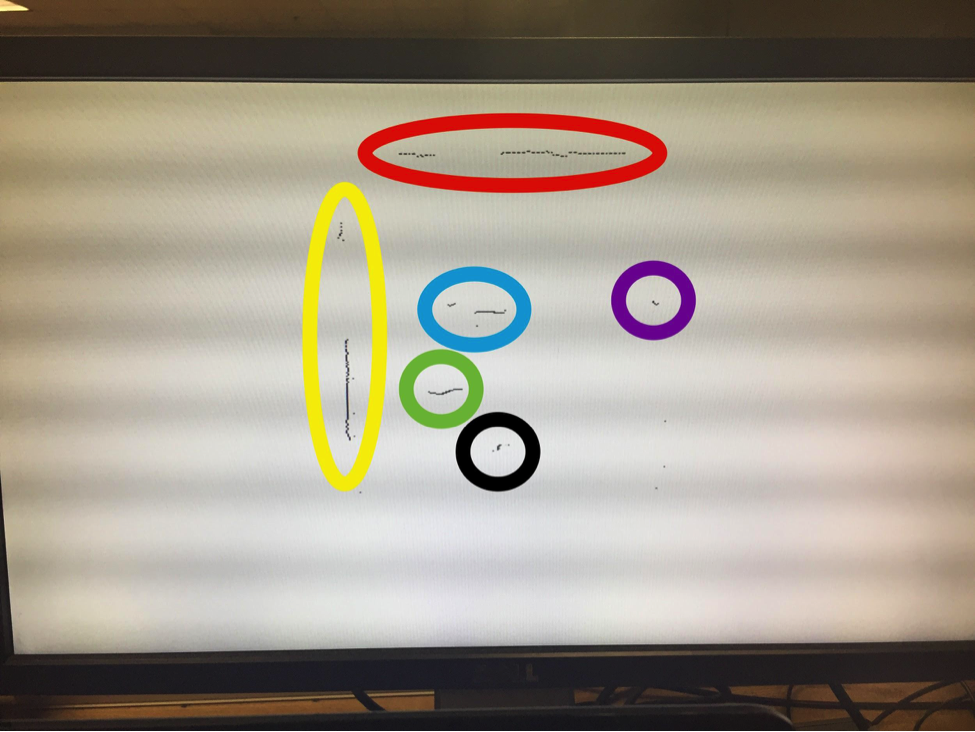
\includegraphics[width=0.75\linewidth]{labtest2_2.png}
		\caption{2D Rangefinder "Floorplan" of Lab at WPI with $180^\circ$ Change of Orientation}
		\label{floorplan2}
	\end{subfigure}
	\caption{Second Lab Test of Rangefinder Functionality}
	\label{labtest2}
\end{figure}

In Figure \ref{labtest2}(\subref{floorplan2}) the black circle is around the rangefinder, the yellow is circling the wall, and the blue is circling the computer and oscilloscope. The green is circling my body while the rangefinder's data capture was being triggered\footnote{Note that I am not shown in Figure \ref{labtest2}(\subref{lab2}) because I moved in order to take the photo.}. The red is circling the windows, and the purple is circling a support beam in the middle of the lab.
\par
Next, the screen was cleared once more. The rangefinder was moved to the first orientation once more to capture data, and then was rotated to the second orientation without clearing the screen. Figure \ref{resultant} shows the resultant VGA output.

\begin{figure}[H]
	\centerline{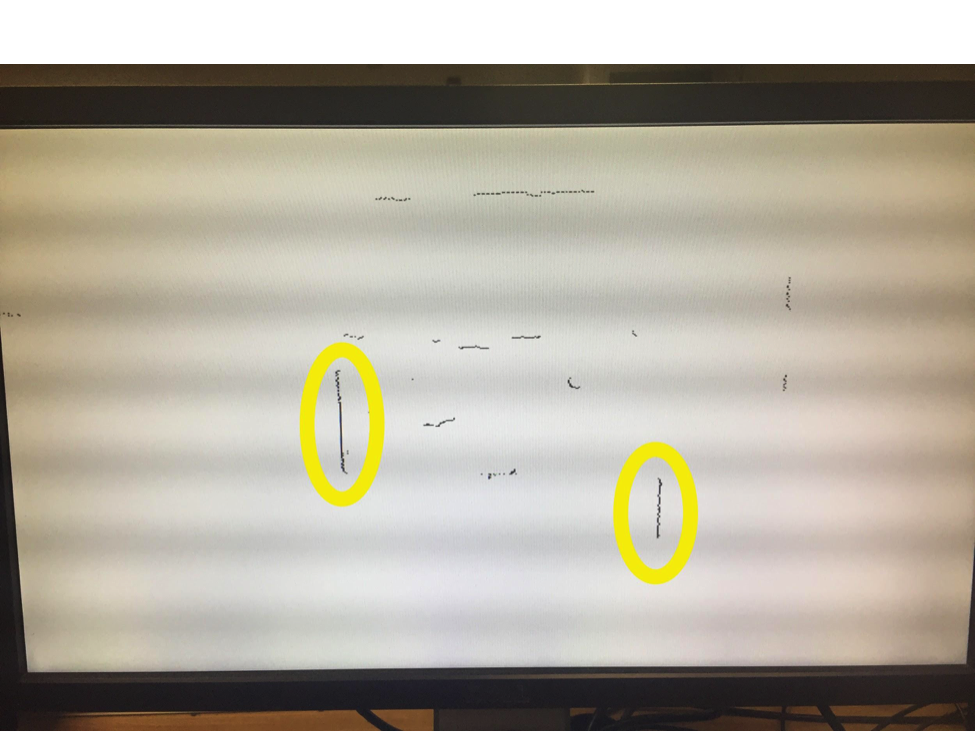
\includegraphics[width=.8\textwidth]{resultant.png}}
	\caption{Two Overlaid Rangefinder "Floorplan" Captures with $180^\circ$ Offset}
	\label{resultant}
\end{figure}

Both rangefinder data captures were triggered successfully and without loss of data. Despite the $180^\circ$ change of orientation, both data captures were overlaid on top of each other. Note that the walls circled in yellow are actually the same wall. This issue was resolved by incorporating the IMU's rotational data. With the IMU's rotational data used to offset the direction of the device, 2D floorplan accurately reflected the relative location of objects.





\subsection{IMU Testing}
The PmodNAV IMU is a small device that was directly connected to the ZedBoard's Pmod connector. As such, it required no external power source or other intermediate connections.

\subsubsection{Communication Testing}
With the rangefinder connected to the ZedBoard's PS MIO Pmod, JE, the PmodNAV IMU required an Extended MIO Pmod so that it could still be controlled by the PS. As such, the SPI pins were routed to the JD Pmod. Since the only slave this project used on the PmodNAV was its magnetometer, the slave select and register settings were adjusted accordingly, as discussed in Section \ref{imu_settings}. To choose the magnetometer and deselect the accelerometer/gyroscope and barometer, the magnetometer's slave select was brought low for each SPI transfer while the other two were left high. The behavior of Pmod JD's pins were observed with an oscilloscope during an SPI transfer. It was observed that as soon as the magnetometer's slave select line was asserted there was unidentified behavior with all of the other pins. Since the PmodNAV was disconnected this issue was thought to be with routing the SPI pins to EMIO incorrectly, so it was decided to test the SPI transfer via Pmod JE.
\par
The pins were re-routed to the MIO Pmod JE and similar undefined functionality was observed when the magnetometer's slave select line was asserted. The ZedBoard's SPI errata was investigated until AR\# 47511 was found, which describes an unresolved issue in the MIO interface where the SPI controller resets itself when slave select 0 signals asserts \cite{zedboardErrata}. Since this issue affected the PS SPI controller itself, this errata was also the cause of the EMIO's undefined behavior.
\par
To avoid the problems with SPI on the ZedBoard, I\textsuperscript{2}C was attempted next, since the PmodNav supports I\textsuperscript{2}C communication. I\textsuperscript{2}C was routed to Pmod JD. Communication with the PmodNAV's magnetometer was tested through I\textsuperscript{2}C, but it was learned that the magnetometer was inaccessible through the I\textsuperscript{2}C bus. As such, SPI was the only option and needed to be implemented.
\par
The SPI pins were again routed to Pmod JD. To avoid the errata, slave select 1 was assigned to the magnetometer. The other two slave select pins were routed away from Pmod JD so that they were not used in any manner. Instead, two GPIO pins were used and configured as pull-ups so that these pins idled high and never had to be written to. This setup was configured in Vivado's Synthesis tab, as shown in Figure \ref{emio_config}. 

\begin{figure}[H]
	\centerline{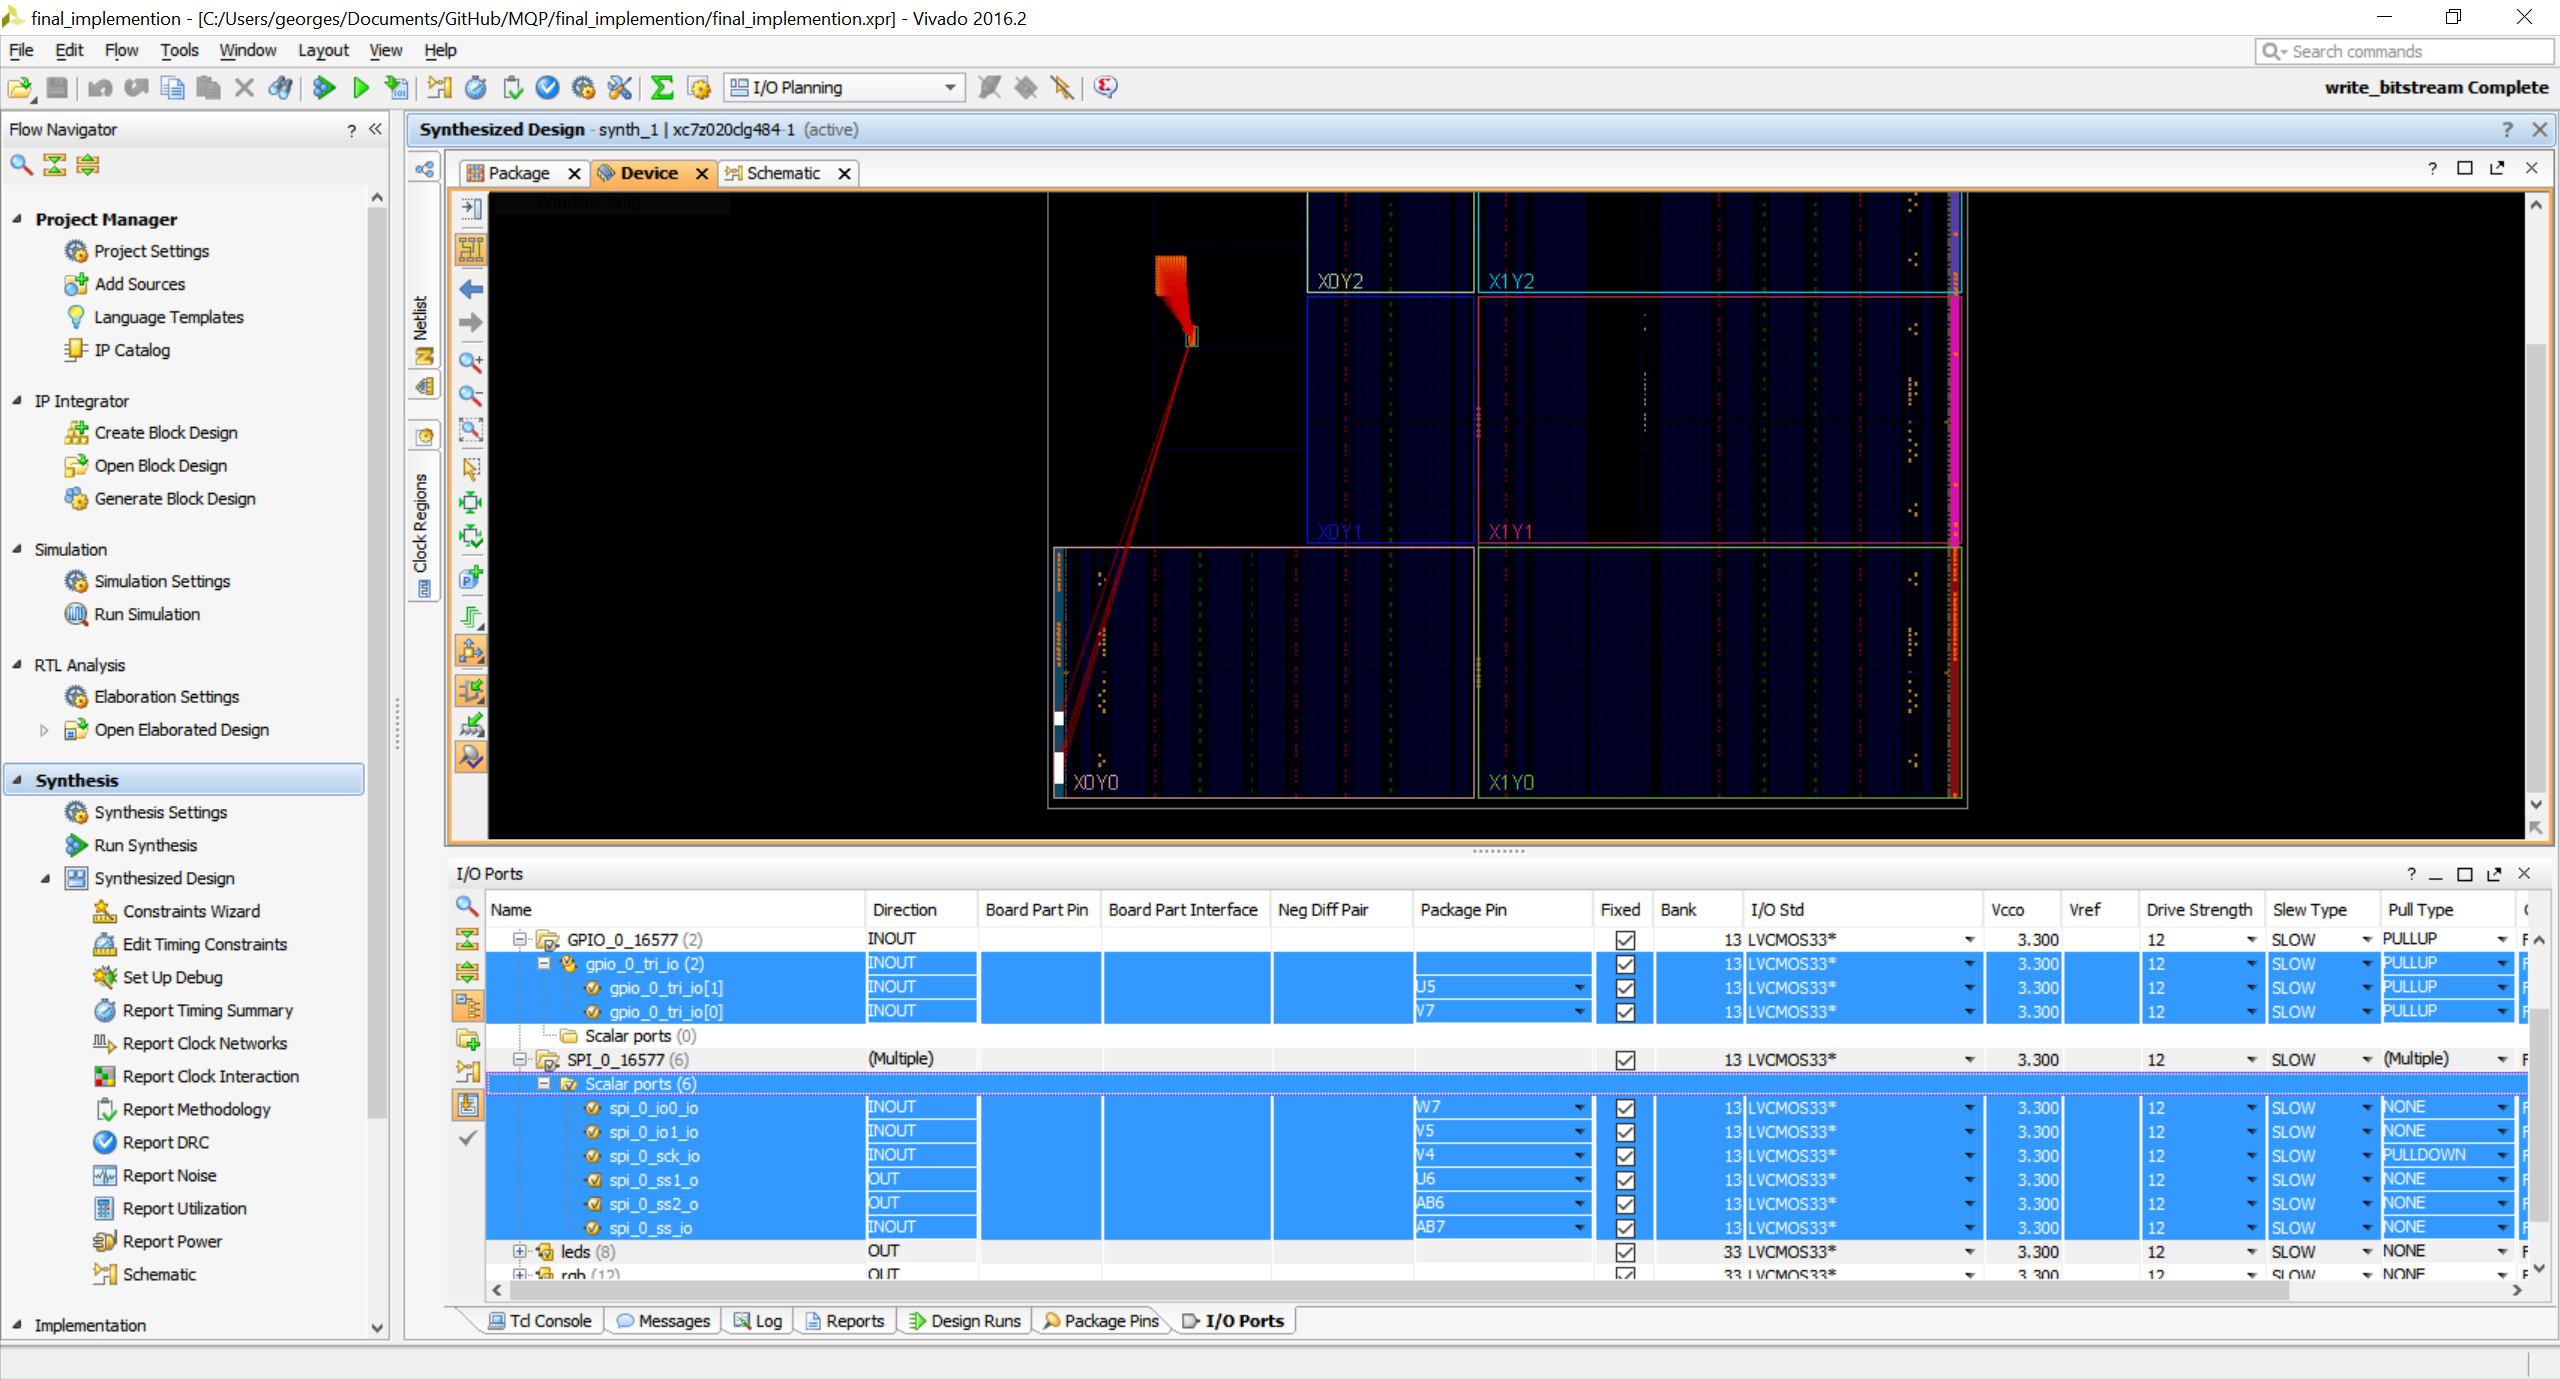
\includegraphics[width=1.1\textwidth]{editing_emio_pins.png}}
	\caption{EMIO SPI Configuration for PmodNAV}
	\label{emio_config}
\end{figure}

With this configuration a waveform similar to those shown in Figures \ref{magnetometer_spi} and \ref{multiple_reads}, were observed, indicating that the errata was avoided and the the master's SPI waveforms were accurate. The PmodNAV was connected to the ZedBoard and successful communication was observed on the oscilloscope, as shown in Figure \ref{OTPHJ}.

\begin{figure}[H] 
	\begin{subfigure}{1\textwidth}
	\centering
		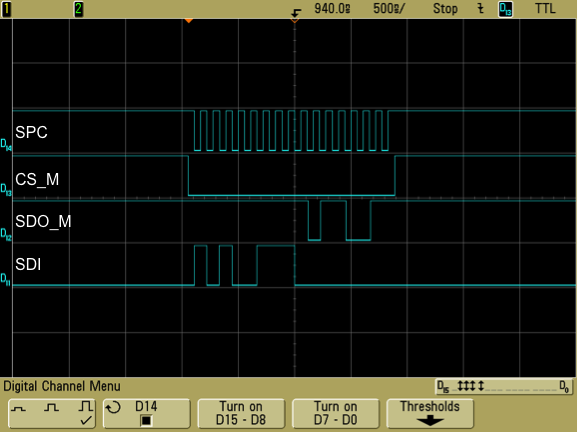
\includegraphics[width=0.75\linewidth]{magSingleRead_label.png}
		\caption{IMU Magnetometer Single Read Operation}
	\end{subfigure}
	\begin{subfigure}{1\textwidth}
	\centering
		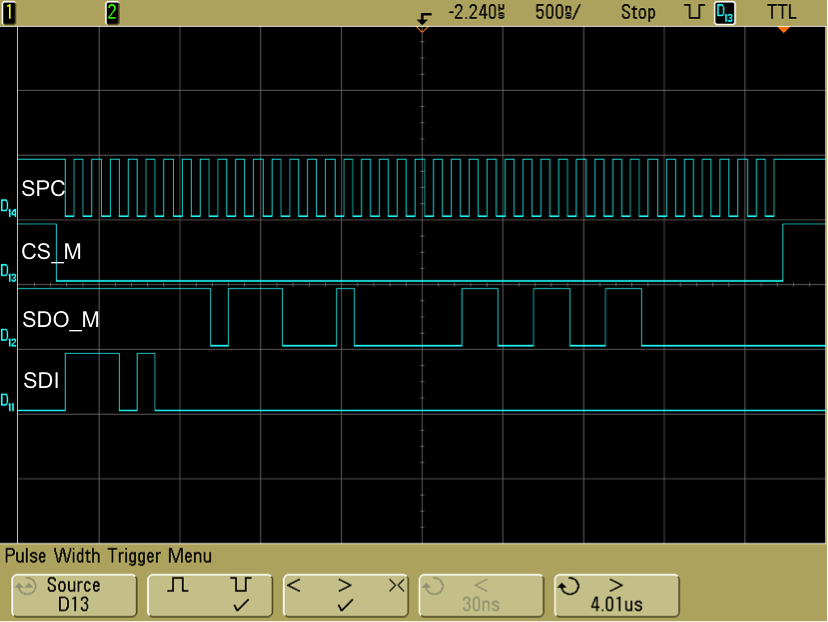
\includegraphics[width=0.75\linewidth]{magMultRead_label.png}
		\caption{IMU Magnetometer Multiple-Byte Read Operation}
	\end{subfigure}
	\caption{Successful IMU Communication via EMIO SPI}
	\label{OTPHJ}
\end{figure}

\subsubsection{Data Testing}
The IMU's data was tested by transmitting it via UART after its data processing. By the end of its data processing, the magnetometer's data was transformed into a compass heading. The ZedBoard's UART was routed to USB UART and connected to a serial console. The sensor suite was rotated, and the compass heading was observed. The results were inaccurate and inconsistent until the sensor suite was moved as far from the lab bench as the wires allowed. The PmodNAV was a very sensitive piece of equipment that was susceptible to electromagnetic interference, in this case most noticeably by the ZedBoard's own power supply. Once the device was further away from the lab bench, accurate and repeatable compass headings were observed.

\subsubsection{Interfacing with the ADIS16375 IMU}
Although this project ultimately interfaced with the PmodNAV IMU, this was not the first IMU that communication was attempted with. Originally, the ADIS16375 Six Degrees of Freedom Inertial Sensor, shown in Figure \ref{adis16375}, was intended to be used in the sensor suite.

\begin{figure}[H]
	\centerline{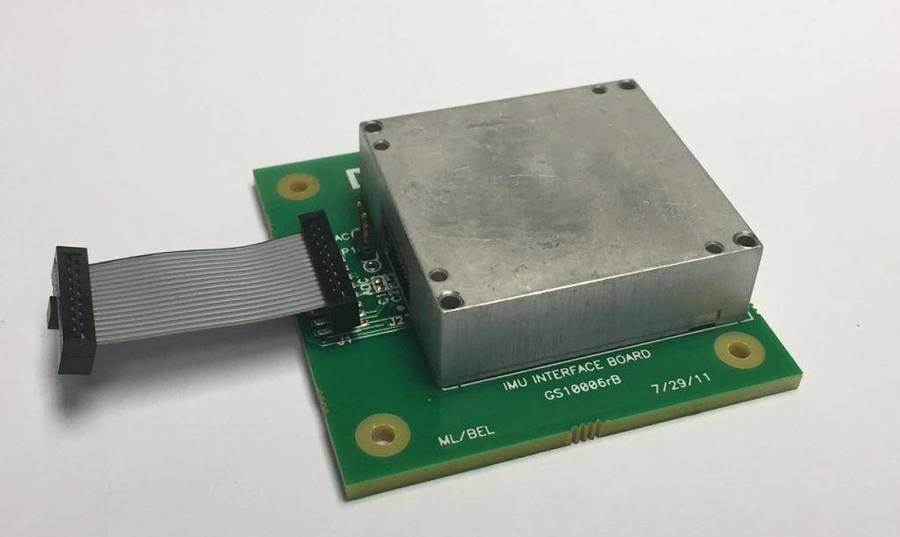
\includegraphics[width=.7\textwidth]{adis16375.jpg}}
	\caption{The ADIS16375 Six Degrees of Freedom Inertial Sensor \cite{adisBreakout}}
	\label{adis16375}
\end{figure}

The ADIS16375 IMU was a highly sensitive, heavy duty device. It had a tri-axis gyroscope, a tri-axis accelerometer, and a temperature sensor, had onboard functionality to calculate delta-angle and velocity, and used SPI communication. Although the ADIS16375 did not have a magnetometer, its gyroscope's sensitivity combined with its sample rate and onboard delta-angle calculation made it perfect to account for rotation. However, communication was not able to be established with it. There was no way to test the ADIS16375 so its functionality could not be confirmed in any manner. instead, the PmodNAV was implemented as a quicker and simpler solution.





\subsection{Single Camera Testing}
After obtaining two of the MT9V034 cameras chosen through the process referenced in Appendix item \ref{camdecision}, several steps were taken to obtain test images from each camera. These steps are outlined in the following sections.
\par
According to the MT9V034 datasheet, each camera module needs to be supplied with an external Master Clock and Output Enable signal in order to operate \cite{mt9v034}. A simple Verilog module for the Nexys3 Spartan-6 FPGA board was created in order to supply the camera module with a 24MHz master clock signal, and a switch was used to toggle output enable. With this module implemented, the camera module's default outputs could then be observed. In order to interface the camera module with an FPGA, the breakout board shown in Figure \ref{camBreakoutBoard} was also created to make the module's pins more easily accessible. 

\begin{figure}[H]
	\centerline{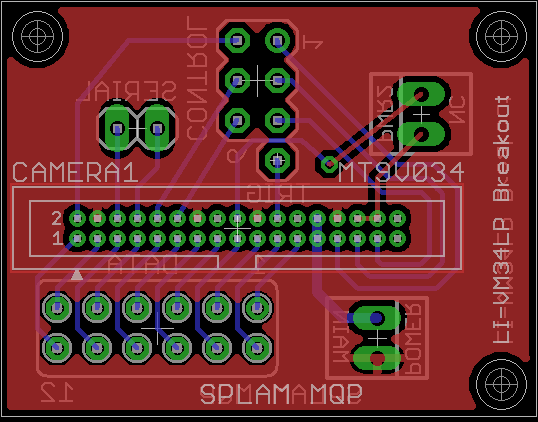
\includegraphics[width=0.5\textwidth]{camera_board.png}}
	\caption{LI-VM34LP Breakout Board}
	\label{camBreakoutBoard}
\end{figure}

\subsubsection{I$^2$C Control} 
Although the MT9V034 camera control registers are closed source, the previous model's registers are available in the camera module datasheet, and have been found to work with the current model thus far \cite{mt9v032}. As a baseline, the camera module was sent a read request at address 0x00, which should return 0x1324 for the MT9V034 camera module. An oscilloscope screenshot of this request is shown in Figure \ref{camVersion}, with the first packet consisting of a request to address 0x00 of device 0x058, and the second packet consisting of the camera's response of 0x1324. 
\begin{figure}[H]
	\centerline{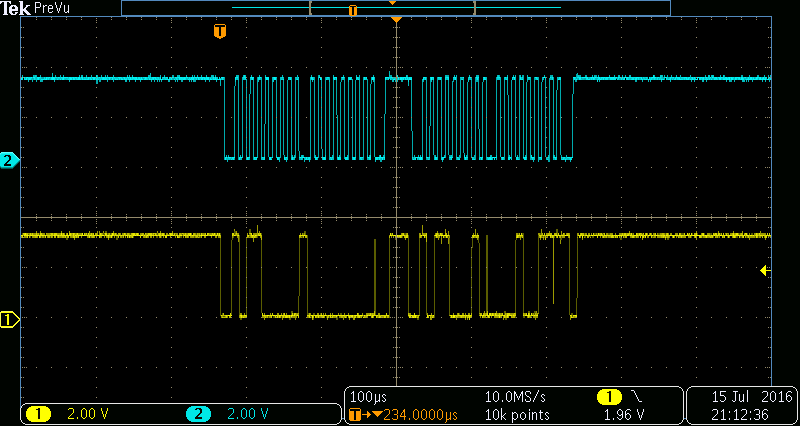
\includegraphics[width=1.0\textwidth]{oScope/i2c_0x00/tek00001.png}}
	\caption{Example I$^2$C Transfer with Camera}
	\label{camVersion}
\end{figure}

\par
After the camera I$^2$C was deemed working, the camera control register needed to be modified to put the camera in "snapshot" mode. In this mode, the camera module will no longer continuously take pictures, and will only gather new images when an external trigger is activated. This is the mode that each camera will need to operate in in order to acquire stereo imagery, since a shared trigger line will allow for both cameras to be controlled simultaneously.
\par
According to the previous camera iteration's datasheet, the camera module's operational mode can be set through control register 0x07. By default, this register will be set to a value of 0x0388, which corresponds to master mode with parallel output and simultaneous readout of pixel data enabled \cite{mt9v032}. In order to put the camera in trigger mode, the control register needs to be written with value 0x0198, which allows for the same functionality as before with the exception of having continuous shutter mode replaced with an external trigger. For reference, a table with bit descriptions for the camera control register can be found in Appendix item \ref{camctlreg} \cite{mt9v032}.
\par
A button input was then attached to the camera's TRIGGER input line, and the TRIGGER and FRAME\_VALID lines were observed on channels one and two of the oscilloscope, as shown in Figure \ref{camInTrigMode}. This oscilloscope screenshot can be seen as an example of how the camera is no longer in continuous operation, since FRAME\_VALID only asserts itself in response to a TRIGGER input. 
\begin{figure}[H]
	\centerline{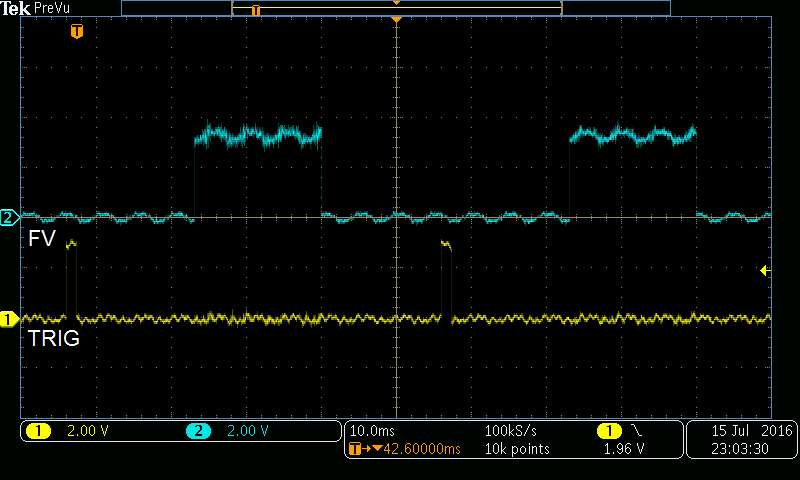
\includegraphics[width=1.0\textwidth]{oScope/i2c_0x07/externalTrigger/externalTrig.png}}
	\caption{Camera Trigger and FV in Trigger Mode}
	\label{camInTrigMode}
\end{figure}
\par
In order to prevent accidental modification of the camera module's configuration registers, the register lock feature of the camera I$^2$C bus is also used. By writing 0xDEAD to register 0xFE, it is possible to disable the I$^2$C bus from being written to. This feature is disabled when the power of the camera module is cycled, or by writing 0xBEEF to the register lock register.
\subsubsection{Data Management}
After successfully creating a camera control interface and placing the MT9V034 camera module in trigger mode, it was then possible to begin viewing images from the module. With the inclusion of the external FIFO module, it is  possible to capture and store an image for future reading, and to read out image data in chunks. Keeping this in mind, the system shown in Figure \ref{camTestBDG} was created for capturing, storing, and transmitting camera images to a computer for external analysis. In order to reduce development time, an external microcontroller was used for controlling the camera module's I$^2$C interface and placing the module in trigger mode. Various buttons and switches on the FPGA were then used for controlling the camera output and trigger, allowing for a user to trigger an image for storage on the AL422B FIFO. Once the image has been stored on the FIFO, the FPGA is capable of reading the image line-by-line into an internal buffer. An internal System on Chip (SoC) is used to control FPGA reads from the FIFO into this internal buffer. An image dump will begin when the SoC microcontroller signals to the FPGA to read a new line of pixels into its internal 8 bit by 752 address pixel buffer. The FPGA will then signal to the microcontroller when this buffer has been filled, and the microcontroller will print out the value of each pixel in the buffer to a connected computer over a Universal Asynchronous Reciever/Transmitter (UART) port. When the microcontroller finishes printing out the value of each pixel in the line buffer, it will signal to the FPGA to read in a new line of pixels. This process will repeat for each of the 480 lines of pixels in the image, allowing for the transmission of an entire image's worth of data from FIFO to computer. The Verilog implementation of the top module and line buffer for this interface can be found in Appendix item \ref{mt9v034TestCode}.

\begin{figure}[H]
	\centerline{\includegraphics[width=1.2\textwidth]{camTestBlockDiag.png}}
	\caption{Camera Test System Block Diagram}
	\label{camTestBDG}
\end{figure}
\par
An example of the transmission of one line of pixel data from the FIFO to the FPGA is shown in Figure \ref{fifoDataOut}.  The green, purple, blue, and yellow lines in this image represent pixel data, FIFO read enable, read reset, and read clock, respectively. Since the FPGA reads in one line of pixel data at a time, this process will take 752 read clock cycles, as measured in Figure \ref{fifoDataOut}. In order to simplify debugging, an internal counter and seven-segment display controller have also been implemented on the FPGA, and will display a running count of the number of pixel lines that have been read into the FPGA's internal buffer, ranging from 0x0000-0x01E0 (0-480). 
\begin{figure}[H]
	\centerline{\includegraphics[width=1.0\textwidth]{oScope/camera_fifo/fifo_rstAndDataTimed.png}}
	\caption{Transferring Line Data from FIFO to FPGA}
	\label{fifoDataOut}
\end{figure}

\subsubsection{Transmitting Images Over UART for Analysis} \label{UARTimg}
Once the FIFO and FPGA line buffer interfaces were created, the source code found in Appendix item \ref{camTestC} was implemented on a Microblaze SoC in order to transmit camera line data from the FPGA's internal line buffer over UART. An example of the microcontroller's UART output is shown in Figure \ref{PuTTYfifoData}. The microcontroller will print the value of each pixel followed by a newline and carriage return, starting with the top left pixel in the acquired image. 
\begin{figure}[H]
	\centerline{\includegraphics[width=0.8\textwidth]{oScope/camera_fifo/PuTTy.png}}
	\caption{Reading FIFO Data}
	\label{PuTTYfifoData}
\end{figure}
\par
After the image is received through PuTTy, the \textsc{Matlab} script found in Appendix item \ref{camTestMatlab} is used to parse the corresponding logfile into a greyscale image. An example image created through this process is shown in Figure \ref{notebookImage}. Note that the sub-optimal quality of this image is due to signal interference and degradation in the test setup's long wiring, as shown in Figure \ref{camTestSetup}. 
\begin{figure}[H]
	\centerline{\includegraphics[width=0.75\textwidth]{oScope/camera_fifo/notebook.png}}
	\caption{Notebook With Grid and Oscilloscope Leads}
	\label{notebookImage}
\end{figure}
\par
Although this system was tested using the Nexys3 (Spartan-6) FPGA board, the use of an external FIFO and little to no platform-specific hardware make it so that it can easily be implemented on any system, including the Zynq family of processors that are used in the final system implementation.   
\begin{figure}[H]
	\centerline{\includegraphics[width=0.75\textwidth]{oScope/camera_fifo/camTestSetup.jpg}}
	\caption{Camera Test Setup}
	\label{camTestSetup}
\end{figure}

\subsection{Final Camera Hardware Implementation}
After successfully gathering image data from a single camera module, an interface needed to be created for controlling both cameras at once using the ZedBoard. Interfacing each camera module directly to the ZedBoard's GPIO is not feasible, since the pair would consume every available PMOD pin on the board, leaving no additional pins for the IMU or rangefinder\footnote{$[2*(D[9:0]+TRIGGER+OE+RST+SCLK+PCLK+FV+LV)]+SDA+SCL = 36\,\,pins$}. One solution originally investigated was the use of the ZedBoard's FPGA Mezzanine Card (FMC) connector, since it contains 68 available GPIO pins and would be more than adequate for interfacing the stereo cameras with the board. However, the FMC connector has been configured to provide logic voltage levels of only 1.8 or 2.5 volts without modification to the ZedBoard. Since each camera module is only compatible with 3.3 volt logic, the FMC connector is therefore not feasible for our designs.
\par
This leaves the final option of reducing the overall pin count required by the cameras and interfacing the combined camera setup with the board's PMOD pins. One significant method of reducing the necessary pins required is to include an individual AL422B FIFO per camera. Based on the testing described in the previous section, it has already been determined that these FIFO modules are compatible with the MT9V034 cameras, and are capable of significantly reducing memory requirements on the FPGA. A second major advantage of including these FIFO modules in the camera interface is that their data output lines may be placed in a high-impedance state. This means that the individual data output lines of each FIFO module can be connected in parallel, with a single FIFO driving the lines at a time. Since the bulk of each camera module's required pin count lies in its data lines, the ability to connect these lines in parallel reduces the overall camera GPIO requirements by 8 pins. Since each AL422B FIFO module is capable of being read from at a clock speed of up to 50MHz and the maximum master clock rate of each MT9V034 camera module is 27MHz, the inclusion of the FIFO modules also won't cause a significant decrease in the overall speed of the stereo camera system \cite{al422b,mt9v034}.
\par
Along with the shared camera data lines between each AL422B FIFO module, it is also possible to connect several other signals in parallel. Since each camera image capture should be triggered at approximately the same time in a stereo imaging setup, it is already desirable to connect both camera TRIGGER lines together. The RST, OE, SDL, SCA, and SCLK lines of each camera module can also be tied together in pairs of two, and the OE lines can simply be held at 3.3 volts. Lastly, since each camera LV signal must be inverted for use with the AL422B FIFOs, a discrete inverter IC may be used to save on FPGA GPIO. Overall, these modifications will save a total of 25 pins, as shown in Equation \ref{lowerPincount}.
\begin{equation}
\label{lowerPincount}
\begin{split}
36\,\, Pins - (8\,\,Data + 4 \,\,truncated\,\,bits) - (TRIGGER+SCLK+RST) \\ - 2*(OE+PCLK+FV+LV) = 13\,\,pins\,(!) 
\end{split}
\end{equation}
\par
Note each FIFO must be controlled individually, requiring an additional Read Reset (RRST) and Read Enable (RE) pin per camera, as well as a shared Read Clock (RCK) line. This brings the total pin count required by the stereo camera setup to 16 pins plus two I2C pins, which is conveniently the number of GPIO available in two PMOD headers. This setup was implemented as shown in Appendix item \ref{stereoCameraSchematic}, and the final stereo camera breakout board shown in Figure \ref{stereoCameraBoard} was then created.  
\par
A Verilog module was created using a modified version of the MT9V034 camera test code found in Appendix item \ref{mt9v034TestCode} and a VGA controller in order to test the stereo camera breakout board. A switch input is used to select one of the two camera modules for image aquisition, and a binned 60x92 pixel set from the center of the camera's image is buffered locally for VGA display. The image is then independently written to the display according to internal VGA timing. This process is repeated at a high rate of speed, allowing for a realtime video stream from the selected camera to be displayed. The assembled stereo breakout board used in this test is shown in Figure \ref{stereoTestSetup}.
\begin{figure}[H] 
	\begin{subfigure}{1\textwidth}
	\centering
		\includegraphics[width=0.65\linewidth]{stereo_top.png}
		\caption{PCB Top}
	\end{subfigure}
	\begin{subfigure}{1\textwidth}
	\centering
		\includegraphics[width=0.65\linewidth]{stereo_board_assembled.JPG}
		\caption{Assembled PCB}
	\end{subfigure}
	\caption{Stereo Camera PMOD PCB}
	\label{stereoCameraBoard}
\end{figure}
\par
\begin{figure}[H] 
	\centering
	\includegraphics[width=0.8\linewidth]{stereo_breakout.JPG}
	\caption{Stereo Camera Breakout Under Test}
	\label{stereoTestSetup}
\end{figure}
\par
After attempting to manually focus each camera using the VGA module described above, the code used in Section \ref{UARTimg} was used to transmit image data from the stereo cameras to a computer for further analysis. As you can see from the example image in Figure \ref{newBoardImage} below, the new stereo camera setup is far less susceptible to data loss in comparison to the previous version. 
\begin{figure}[H] 
	\centering
	\includegraphics[width=0.8\linewidth]{cam1_image.png}
	\caption{Stereo Camera Breakout Sample Image}
	\label{newBoardImage}
\end{figure}
\par
For further comparison, please refer back to the test image acquired using the original camera test setup, as shown in Figure \ref{notebookImage}.
\subsubsection{Image Buffering}
\begin{figure}[H] 
	\centering
	\includegraphics[width=0.8\linewidth]{bram_test.JPG}
	\caption{ZedBoard BRAM Camera Test}
	\label{bramCamTest}
\end{figure}
\subsection{Disparity Testing}
After verifying that the camera interface was functional, a large portion of time was spent implementing a disparity algorithm that would allow for the extraction of 3D depth information from stereo image data. This algorithm was first implemented in \textsc{Matlab}, and was then transferred to programmable logic after the algorithm was verified working. 
\subsubsection{Image Rectification}
In order to perform the most accurate block matching as possible on camera image data, it would be ideal to rectify the images as outlined in Section \ref{rectsec}. 
\par
- ADD AN EXAMPLE OF THE MATLAB CALIBRATION STUFF (figures showing 3d anaglyph process)\par
- TALK ABOUT WHY WE DIDNT USE IN FINAL IMP


\subsubsection{\textsc{Matlab} Impelmentation}


\subsubsection{Verilog Test Bench}
The original disparity test implementation used closely follows the \textsc{Matlab} disparity algorithm shown in Appendix item \ref{disparityTestMatlab}. This algorithm is implemented using a finite state machine with five states, as shown in Figure \ref{disparityTestImp} below. In order to maintain simplicity, the test algorithm has been implemented to operate on 46x30 windowed portions of the input imagery. By default, the disparity module will remain in an idle state until an external enable signal is toggled high using a button input. This will cause the finite state machine to advance to its READ state, and image data for the left and right camera images will be read in from the stereo camera breakout board. After image data has been received, the state machine will then advance to a cyclical set of states used for iterating through each image and calculating disparity. 
\par
The disparity module will begin by isolating the template and search blocks from the right and left image data in the finite state machine's separation state. Next, the state machine will advance to its SAD state, and will calculate the sum of absolute differences between the template and search block. This value is placed in a vector that matches the length of the search range. If the vector hasn't been completely filled, indicating that there are more search blocks to compare to the template, the state machine will revert back to the separate state, isolating a new search block from the right camera image. When the SAD vector is full, the state machine will advance to its finalization state. 
\par
\begin{figure}[H]
	\centerline{\includegraphics[width=0.75\textwidth]{looping_disparity.png}}
	\caption{Disparity Test Implementation}
	\label{disparityTestImp}
\end{figure}
\par
The finalization state is used to search through the SAD vector for the lowest value. The index of this value within the SAD vector in reference to the template block location is used to create a disparity value for the given template block location. This value is then converted to a distance using Equation \ref{disp2dist}, and is stored in the output image location. If the output image hasn't been fully populated with distance values, the state machine will then revert back to the separate state. Otherwise, the state machine will advance to its idle state, and the resulting disparity image can be read for output. 
\par
This module was initially tested using a verilog test bench, and was then tested using camera image data and a VGA display controller module, allowing for real-time verification of the algorithm's effectiveness. After testing the initial disparity algorithm, several modifications were made to increase the overall speed and efficiency of the disparity module. 
\subsubsection{Test Bench Results}
\begin{figure}[H]
	\centerline{\includegraphics[width=1.25\textwidth]{disp_tb/disparity_vector.png}}
	\caption{Disparity Search Vector}
	\label{disparityVector}
\end{figure}

\begin{figure}[H]
	\centerline{\includegraphics[width=1.25\textwidth]{disp_tb/disparity_fullPixelRow.png}}
	\caption{Horizontal Pixel Row Search}
	\label{disparityRowSearch}
\end{figure}

\begin{figure}[H]
	\centerline{\includegraphics[width=1.25\textwidth]{disp_tb/full_disparity.png}}
	\caption{Full Image Search}
	\label{disparityFullSearch}
\end{figure}

\begin{figure}[H]
	\centerline{\includegraphics[width=1.0\textwidth]{disp_tb/result_gray.png}}
	\caption{Disparity Test Results}
	\label{disparityTestResults}
\end{figure}

\begin{figure}[H]
	 \begin{subfigure}[h]{1.0\textwidth}
             \centerline{\includegraphics[width=1.2\textwidth]{disp_tb/MATLAB_cones.png}}
             \caption{\textsc{Matlab} Result}
			\label{disparityMatlabResult}
         \end{subfigure} 
         %\\
         \begin{subfigure}[h]{1.0\textwidth}
              \centerline{\includegraphics[width=0.66\textwidth]{disp_tb/tb_cones.png}}
             \caption{Test Bench Result}
			\label{disparityVerilogResult}
         \end{subfigure}
\label{disparityVerilogvsMatlab}
\caption{\textsc{Matlab} vs. Verilog Test Bench Results}
\end{figure}



\subsubsection{Final Implementation}
\begin{figure}[H]
	\centerline{\includegraphics[width=1.2\textwidth]{Disparity_Algorithm.png}}
	\caption{Disparity Final Implementation}
	\label{disparityTestImp}
\end{figure}
\par
\begin{figure}[H] 
	\begin{subfigure}{0.5\textwidth}
	\centering
		\includegraphics[width=0.8\linewidth]{disparity_rtView.JPG}
		\caption{Device View}
	\end{subfigure}
	\begin{subfigure}{0.5\textwidth}
	\centering
		\includegraphics[width=0.8\linewidth]{disparity_rt.JPG}
		\caption{Resultant Disparity}
	\end{subfigure}
	\caption{Disparity Algorithm Output}
	\label{disparityFin}
\end{figure}
\par
GET RID OF CALIBRATION 
%rangefinder and IMU stuff 
% then combined imp after?
\subsection{Combined Implementation}
An overall system block diagram of the final implementation of this project is shown in Figure \ref{finalBD}. This implementation may be broken down into several major components. At the top level, several blocks are used to connect the Zynq7 ARM Cortex A9 processing system to customized programmable logic using an AXI peripheral controller, as well as to peripherals such as the rangefinder and IMU using EMIO-GPIO and SPI-GPIO. 
\par
All programmable logic created for the rangefinder, IMU, and camera interface has been ported to a user-generated IP module named "custom logic", as shown in Figure \ref{finalBD}. This module connects directly to the stereo camera breakout board, and accepts rangefinder and IMU data from the programmable software via an AXI interface. This customized IP core also accepts user inputs through the ZedBoard's switches, and supports outputs to the ZedBoard's LEDs and VGA interface. 
\par
\begin{figure}[!htb] 
	\centerline{
	\includegraphics[width=1.25\linewidth, angle=90]{final_bd.png}
	}
	\caption{System Block Diagram}
	\label{finalBD}
\end{figure}
\par
The final hardware implementation of the project can be found in Figure 
\ref{finalHW}. This implementation supports several output modes based on the positions of the user switches, including a 3D disparity mode, camera image mode, rangefinder output mode, and combined 2D "floorplan" mode. Note that the VGA outputs of each mode are continuously updated in semi-realtime. 
\begin{figure}[H]  
 	\centerline{
	\includegraphics[width=0.85\linewidth]{setup.JPG}
	}
	\caption{System Hardware}
	\label{finalHW}
\end{figure}
\par
The 3D disparity output mode may be found in Figure \ref{disparityOutputs}a. In this mode, a windowed 384x288 pixel depth map is continuously updated to reflect the camera's current field of view. Figure \ref{disparityOutputs}b shows a modified version of this output consisting of depth information from a centrally-located horizontal line of pixels from this depth map that may then be correlated with data from the scanning laser rangefinder. 
\par
\begin{figure}[H] 
         \begin{subfigure}[h]{0.5\textwidth}
              \centerline{\includegraphics[width=1.0\textwidth]{disparity_mode.JPG}}
             \caption{Full Output}
         \end{subfigure}
         \begin{subfigure}[h]{0.5\textwidth}
             \centerline{\includegraphics[width=1.0\textwidth]{disparity_line_mode.JPG}}
             \caption{Single Line Output}
         \end{subfigure}
\caption{Disparity Output Modes}
\label{disparityOutputs}
\end{figure}
\par
In order to aid in hardware debugging, an additional output mode has been included for showing the current camera images being used by the disparity algorithm, as shown in Figure \ref{camOutMode}. Note that the images captured are monochrome, and are being arbitrarily mapped to VGA colors due to a lack of grayscale color space.
\par
\begin{figure}[H]  
 	\centerline{
	\includegraphics[width=0.5\linewidth, angle=-90]{camera_mode.JPG}
	}
	\caption{Raw Camera Data Mode}
	\label{camOutMode}
\end{figure} 
\par
The normal rangefinder output mode is shown in Figure \ref{rangeOutputs}a. In this mode, objects found by the scanning laser rangefinder are displayed in black. The entire scan is also referenced to the device's central location, shown in red. All rangefinder data is also pre-processed by the programmable software to include a compass offset from the IMU, with due north representing the center of the top of the VGA display.
\par 
A final output mode has also been included to incorporate disparity data with the 2D "floorplan" produced by the rangefinder. By combining data from both sensors, the stereo cameras are able to account for situations where the scanning laser rangefinder would be out of range due to its limitations on viewing distance. This output mode is shown in Figure \ref{rangeOutputs}b.

\begin{figure}[H] 
         \begin{subfigure}[h]{0.5\textwidth}
              \centerline{\includegraphics[width=1.0\textwidth]{rangefinder_mode.JPG}}
             \caption{Rangefinder Output}
         \end{subfigure}
         \begin{subfigure}[h]{0.5\textwidth}
             \centerline{\includegraphics[width=1.0\textwidth]{combined_mode.JPG}}
             \caption{Combined Output}
         \end{subfigure}
\caption{2D "Floorplan" Output Modes}
\label{rangeOutputs}
\end{figure}


\newpage 
\section{Conclusions}
This project demonstrated a proof of concept SLAM sensor suite that could be used as a cost-effective replacement for the simple camera image sensors available on existing remote mapping robotic products. Through the use of a stereo camera pair, scanning laser rangefinder, inertial measurement unit, and Zynq-7000 All Programmable SoC, an all-in-one sensor suite was developed that was capable of capturing 2D and 3D data on its surroundings. This sensor suite was unique in that it was able to process all of its data locally, without the need for additional processing power from the end user.
\par
On the input stage of the sensor platform, the scanning laser rangefinder and IMU module were connected directly to the dual-core ARM Cortex A9 processor of the Zynq SoC, and were communicated with using low-level peripheral controls. Data collected from each sensor was passed to the FPGA fabric of the Zynq SoC, where a coordinate-axis transform was used to localize rangefinder data based on IMU readings and prepare it for output via VGA display. In addition, a custom made printed circuit board was used to connect two camera modules and image buffer ICs to the FPGA fabric of the Zynq SoC. After acquiring stereo camera image data, a Sum of Absolute Differences block matching algorithm was used to convert said data to depth measurements on a pixel by pixel basis. This depth information was then exported as-is in the form of a 3D depth map, or in slices combined with rangefinder and IMU data to form a 2D floorplan of the area being observed by the sensor suite. The outputs of this platform demonstrated that FPGA-based data processing was a viable replacement for the simple imaging sensors of existing remote mapping products. 
\par
At the time of submission, the rangefinder, camera, and IMU interfaces and processing stages described were fully implemented and tested in both hardware and various forms of simulation. This project was completed over a shortened timeline, and a larger portion of this time was dedicated to debugging hardware issues than originally expected. Due to a limited project budget of \$250, a customized stereo camera interface PCB with attached frame buffer ICs was developed as a low-cost alternative to existing commercial products. Several issues were encountered with the physical hardware of this interface, and this resulted in lost development time. 
\par
Issues were also encountered with finding a proper method of communicating with the scanning laser rangefinder, as the rangefinder and ZedBoard Zynq evaluation platform used two different logic voltage levels in their UART communications.  After successfully resolving these issues by using a RS232-TTL logic-level converter, development began on integrating data from the inertial measurement unit into the rangefinder interface. After several weeks of unsuccessful communications and debugging with the original IMU intended for use in the project, it was determined that the unit was non-functional. A replacement unit relying on a different IMU sensor was eventually acquired in the final week of development, and little time was left for integrating IMU data into the sensor suite's overall implementation.
\par
Although the issues mentioned resulted in large delays in development, the proof of concept SLAM sensor suite created through this project serves as an excellent platform for future development. The implications of the hardware issues faced in this project were quickly realized, and some recommendations for future work may be based off of original project goals that were modified as a result of time constraints.

\subsection{Future Work}
For this sensor suite to be utilized to its maximum potential, additional image processing algorithms should be implemented to allow for human recognition and object detection. In a first responder situation, human recognition could be used to provide potentially life-saving information about where people are located. With additional IMU data completely integrated, this sensor suite also has the capability to produce a sophisticated 2D map with both the sensor suite's displacement and rotational data, and can even be combined with the stereo cameras' depth and human detection information. This functionality would allow for a near-complete understanding of the environment around the device.
\par
In order for the sensor suite's information to be useful to first responders, it needs to be accessible via wireless transmission. With wireless data transmission, not only is the system unrestricted by a physical connection, but the data can also be accessible by numerous devices at the same time. Since the sensor suite also processes its data locally, the information transmitted would be accessible to a wide range of low-power electronics without any major processing requirement.
\par
To reduce overall size and cost of the system, the completed design could use an integrated printed circuit board containing a Zynq chip, an onboard IMU, and mounted stereo camera hardware. With the creation of a customized sensor board, this project could truly serve its purpose as a durable replacement sensor suite for a wide range of robotic platforms currently used for remote observation and mapping. 






\newpage
\singlespacing
%https://www.sharelatex.com/learn/Bibliography_management_with_bibtex
\begin{thebibliography}{9}

\bibitem{al422b}
Averlogic.
\textit{AL422B Data Sheets}. 2001.
Available from: \url{http://www.frc.ri.cmu.edu/projects/buzzard/mve/HWSpecs-1/Documentation/AL422B_Data_Sheets.pdf}.

\bibitem{davison} 
Davison, A.J.,
\textit{Real-Time Simultaneous Localisation and Mapping with a Single Camera}. 
IEEE Computer Vision, 2003. 2(1).

\bibitem{livm34lp}
Leopard Imaging Inc.
\textit{LI-VM34LP Camera Board}. 2009.
Available from: \url{http://www.leopardimaging.com/uploads/li-vm34lp_v1.1.pdf}.

\bibitem{serveball}
\textit{Serveball}.
Available from: \url{http://www.serveball.com/}.

\bibitem{mattoccia}
Stefano Mattoccia, M.P.,
\textit{A passive RGBD sensor for accurate and real-time depth sensing self-contained into an FPGA}.
in \textit{International Conference on Distributed Smart Cameras}. 2015.

\bibitem{mt9v032}
On Semiconductor. 
\textit{MT9V032: 1/3-Inch Wide-VGA CMOS Digital Image Sensor}. 2015. 
Available from: \url{http://www.onsemi.com/pub_link/Collateral/MT9V032-D.PDF}.

\bibitem{mt9v034}
On Semiconductor. 
\textit{MT9V034: 1/3-Inch Wide-VGA CMOS Digital Image Sensor}. 2015. 
Available from: \url{http://www.onsemi.com/pub_link/Collateral/MT9V034-D.PDF}.

\bibitem{porikli}
Fatih Porikli, O.T.,
\textit{Human Body Tracking by Adaptive Background Models and Mean-Shift Analysis}.
in \textit{IEEE International Workshop on Performance Evaluation of Tracking and Surveillance}. 2003.

\bibitem{thrun}
Sebastian Thrun, D.H., David Ferguson, Michael Montemerlo, Rudolph Triebel, and C.B. Wolfram Burgard, Zachary Omohundro, Scott Thayer, William Whittaker.
\textit{A System for Volumetric Robotic Mapping of Abandoned Mines}. 
in \textit{IEEE International Conference on Robotics and Automation}. 2003.

\end{thebibliography}

% include in ToC - must be after refs for correct page link from hyper
\addcontentsline{toc}{section}{References} %%%% Bibliography %%%%
\doublespacing
\newpage

\section*{Appendix} %%%% Appendix %%%% 
\addcontentsline{toc}{section}{Appendix}
\setcounter{subsection}{0}
\renewcommand\thesubsection{\Alph{subsection}}
\renewcommand\thesubsubsection{\thesubsection.\roman{subsubsection}}
\subsection{Useful Resources}
This section is intended to serve as complete compilation of all resources gathered throughout D Term 2016 that we believe will be useful as we begin to work on the methodology portion of our project.

\begin{itemize}
  \item Strother, Daniel. 2011. "Open-Source FPGA Stereo Vision Core Released." \path{https://danstrother.com/2011/06/10/fpga-stereo-vision-core-released/}.
  
  \item Field, Mike. 2013. "Zedboard OV7670." \path{http://hamsterworks.co.nz/mediawiki/index.php/Zedboard_OV7670}.
  
  \item "OV7670/OV7671 CMOS VGA CameraChip Implementation Guide." \path{https://www.fer.unizg.hr/_download/repository/OV7670new.pdf}.
  
  \item "MIPI CSI2-to-CMOS Parallel Sensor Bridge - Lattice Semiconductor." \path{http://www.latticesemi.com/~/media/LatticeSemi/Documents/ReferenceDesigns/JM/MIPICSI2to CMOSParallelSensorBridgeDocumentation.pdf?document_id=50533}.
  
  \item "OmniVision Serial Camera Control Bus (SCCB) Functional Specification." \path{http://www.ovt.com/download_document.php?type=document&DID=63"}.
  
  \item Morvan, Yannick. "Multiple-View Depth Estimation." \path{http://www.epixea.com/research/multi-view-coding-thesisse15.html}.
  
  \item MathWorks. "Depth Estimation From Stereo Video." \path{http://www.mathworks.com/help/vision/examples/depth-estimation-from-stereo-video.html}.
  
  \item Stefano Mattoccia, Matteo Poggi. 2015. "A passive RGBD sensor for accurate and real-time depth sensing self-contained into an FPGA". International Conference on Distributed Smart Cameras.
  
  \item Mattoccia, Stefano. 2013. "Stereo Vision: Algorithms and Applications." \path{http://www.slideshare.net/DngNguyn43/stereo-vision-42147593}.
  
  \item Szeliski, Richard. 2010. Computer Vision: Algorithms and Applications. New York: Springer.
  
  \item Beau Tippets, Dah Jye Lee, Kirt Lillywhite, James Archibald. 2013. "Review of Stereo Vision Algorithms and Their Suitability for Resource-Limited Systems." Journal of Real-Time Image Processing 11 (1). doi: 10.1007/s11554-012-0313-2.
  
  \item Jouni Rantakokko, Joakim Rydell, Peter Stromback, Peter Handel, Jonas Callmer, David Tornqvist, Fredrik Gustafsson, Magnus Jobs, Mathias Gruden. 2011. "Accurate and Reliable Soldier and First Responder Indoor Positioning: Multisensor Systems and Cooperative Localization." IEEE Wireless Communications 18 (2):10-18. doi: 10.1109/MWC.2011.5751291.
  
  \item Davison, Andrew J. 2003. "Real-Time Simultaneous Localisation and Mapping with a Single Camera."  IEEE Computer Vision 2 (1). doi: 10.1109/ICCV.2003.1238654.
  
  \item Fatih Porikli, Oncel Tuzel. 2003. "Human Body Tracking by Adaptive Background Models and Mean-Shift Analysis." IEEE International Workshop on Performance Evaluation of Tracking and Surveillance.
  
  \item Giovanni Pintore, Enrico Gobbetti. "Effective mobile mapping of multi-room indoor structures."  The Visual Computer 30 (6):707-716. doi: 10.1007/s00371-014-0947-0.
  
  \item "iRobot 110 FirstLook." iRobot. \path{http://www.irobot.com/$~$/media/Files/Robots/Defense/FirstLook/iRobot-110-FirstLook-Specs.pdf}.

\end{itemize}
 % useful resources
\subsection{Component Selection} \label{componentSelection}

\begin{center}
\begin{tabular}{ |c|c|c|c| } 
 \hline
 \textbf{Component} & \textbf{Part Number}  & \textbf{Supplier} & \textbf{Cost}  \\ \hline
 FPGA & ZedBoard & Borrowed & N/A  \\ \hline
 IMU & PmodNav & Digilent & \$45  \\ \hline
 Rangefinder & URG-04LX & Borrowed & N/A  \\ \hline
 RS232 to TTL Converter & MAX232CSE & uxcell & \$7  \\ \hline
 RS232 Breakout Board & Swellder DB9 & VIKINS Tech & \$7  \\ \hline
 Stereo Cameras$^\dagger$ & MT9V034 & Mouser & \$146  \\ 
 \hline
\end{tabular}
\end{center}
$^\dagger$ Note that we originally planned to purchase a flir lepton thermal camera module and accompanying breakout board to support two stereo ov7670 camera modules. After experimenting with the ov7670 camera module on our FPGA board, we began to realize that these camera modules are highly limited due to their low frame rate and poor documentation, and realized that we wanted to search for a different camera module. In addition, at a price of \$223 for a thermal camera with an 80x60 degree resolution, 25 degree fov, and 7-9Hz image sample rate, we believe that we are much better off spending our money on better camera modules that will be more usable for our task. For more information see Section  \ref{camdecision}. % component selection
%\subsection{Camera Module Decision Matrix}
\singlespacing
\begin{small}
\centerline{
\begin{tabular}{ |L{2cm}|L{1.5cm}|L{2.5cm}|L{1cm}|L{1.7cm}|L{2cm}|L{1.7cm}|L{1.2cm}|L{1cm}| } 
 \hline
 \textbf{Camera Module} & \textbf{Max Frame Rate (FPS)}  & \textbf{Resolution at Max Frame Rate (px.)} & \textbf{Cost} & \textbf{Requires External Adapter} & \textbf{Data Transfer Interface} & \textbf{Shutter} & \textbf{Field of View (deg.)} & \textbf{Rank 0-10}  \\ \hline
 OV7670 & \cellcolor{red!25} 30 & \cellcolor{green!25} 640x480 & \cellcolor{green!50} \$10 & \cellcolor{green!25} No & \cellcolor{green!25} Parallel & \cellcolor{red!25} Rolling & \cellcolor{red!25}  25 & 5  \\ \hline
 Raspberry Pi Camera &\cellcolor{green!25}  90 & \cellcolor{green!25} 640x480 & \cellcolor{green!25}  \$30 & \cellcolor{red!25} Yes, \$53 & \cellcolor{red!25} MIPI (CSI2) & \cellcolor{red!25}  Rolling & \cellcolor{green!25} 49 & 6  \\  \hline
 PC1089K & \cellcolor{green!25} 60 & \cellcolor{green!25} 720x480 & \cellcolor{green!25} \$32 & \cellcolor{green!25} No & \cellcolor{red!50} NSTC/ PAL & \cellcolor{red!25} Rolling & Not Given & 5 \\ \hline 
 OV4682 & \cellcolor{green!50} 330 & \cellcolor{green!25} 640x480 & \cellcolor{red!25} \$89 & \cellcolor{red!25} Yes, \$50 & \cellcolor{red!25} MIPI & \cellcolor{red!25} Rolling & Not Given & 6 \\ \hline
 \textbf{MT9V034} & \cellcolor{green!25} \textbf{60} & \cellcolor{green!25} \textbf{750x480} & \cellcolor{red!25} \textbf{\$73} & \cellcolor{green!25} \textbf{No} & \cellcolor{green!25} \textbf{Parallel} & \cellcolor{green!50} \textbf{Global} & \cellcolor{green!25} \textbf{55} & \textbf{9} \\ \hline   
\end{tabular} }
\par
For purposes of comparison, the thermal camera module we were evaluating is also shown below.
\centerline{
\begin{tabular}{ |L{2cm}|L{1.5cm}|L{2.5cm}|L{1cm}|L{1.7cm}|L{2cm}|L{1.7cm}|L{1.2cm}|L{1cm}| } 
\hline
Flir Lepton &  \cellcolor{red!50} 9 & \cellcolor{red!50} 80x60 & \cellcolor{red!25} \$175 & \cellcolor{red!25} Yes, \$40 & \cellcolor{green!25} SPI/ MIPI & N/A & \cellcolor{green!25} 50 & 3 \\ \hline 
\end{tabular} 
}
\end{small}
\par
Shown above is our decision matrix for choosing a camera module. Fields marked in green indicate a positive ranking, while red indicates a negative ranking. Based on the individual rankings of each item's field, we gave our camera modules an overall ranking of 0-10 in the right hand column, with 10 being an extremely high ranking and 0 being an extremely low ranking.
\doublespacing
\par
Based on our decision matrix, we believe that it would be worth both our time and money to use the MT9V034 camera modules for our stereo camera interface. These camera modules are the only low-cost global shutter option we've come across, and would be ideal for taking images in a sensor suite that is susceptible to motion. The MT9V034 also uses a parallel data interface and relies on an external clock and shutter trigger, making the module ideal for interfacing with an FPGA-based stereo imaging setup.
 % camera module decision matrix
\subsection{Camera Module Control Register} \label{camctlreg}
\begin{figure}[H]
	\centerline{\includegraphics[width=1.0\textwidth]{CamControlReg.PNG}}
	Table obtained from MT9V032 Datasheet \cite{mt9v032}
\end{figure}
\newpage
\subsection{Stereo Camera Schematic}\label{stereoCameraSchematic}
\begin{figure}[H]
	\centerline{\includegraphics[width=1.0\textwidth]{stereo_schematic.png}}
\end{figure}
\newpage
% maybe redo this so we have a section called "code" and
% subsections for individual projects?
\subsection{Code}

\subsubsection{MT9V034 and Al422b Test Code} \label{mt9v034TestCode}
\textbf{Top Module:}
\singlespacing
\lstinputlisting[style=Verilog]{appendix/verilog/mt9v034_test_top.v}
\doublespacing
\par
\textbf{Local Data Buffer:}
\singlespacing
\lstinputlisting[style=Verilog]{appendix/verilog/mt9v034_test_buffer.v}
\doublespacing
\par
\textbf{MicroBlaze Code:}
\label{camTestC}
\singlespacing
\lstinputlisting[style=C]{appendix/c/imageUART.c}
\doublespacing
\par
\textbf{\textsc{Matlab} Image Parser:}
\label{camTestMatlab}
\singlespacing
\lstinputlisting[style=Matlab]{appendix/matlab/ParseData.m}
\doublespacing
%%%%%%%%%%% end mt9v034 test code %%%%%%%%%% 

\subsubsection{Custom IP} 
\textbf{Top Module:} \label{customIPtop}
\singlespacing
\lstinputlisting[style=Verilog]{appendix/verilog/nu_nu_rangefinder_vga_v1_0.v}
\doublespacing

\par
\textbf{Instantiated File:} \label{customIPaxi}
\singlespacing
\lstinputlisting[style=Verilog]{appendix/verilog/nu_nu_rangefinder_vga_v1_0_S00_AXI.v}
\doublespacing

\subsubsection{Disparity Algorithm Implementation} \label{disparityTestMatlab}
\textbf{\textsc{Matlab} Algorithm:}
\singlespacing
\lstinputlisting[style=Matlab]{appendix/matlab/stereoDisparity.m}
\doublespacing

\par
\textbf{\textsc{Verilog} Algorithm:}
\singlespacing
\lstinputlisting[style=Verilog]{appendix/verilog/disparity.v}
\doublespacing
%\subsection{\textsc{Matlab} Code}
\subsubsection{Camera Image Parsing} \label{camTestMatlab}
\singlespacing
\lstinputlisting[style=Matlab]{appendix/matlab/ParseData.m}
\doublespacing
%\newpage
%\subsection{Verilog Code}
%\newpage
%\subsection{C Code}
\subsubsection{Camera Image Parsing} \label{camTestC}
\singlespacing
\lstinputlisting[style=C]{appendix/c/imageUART.c}
\doublespacing
%\newpage
%\subsection{Coefficient Files}
\subsubsection{LUT Initialization Code for Transformation from Polar to Cartesian} \label{coe_file}
\textbf{Coefficient File for $0^\circ{}\leq{}\theta{}\leq45^\circ$}
\singlespacing
\lstinputlisting[style=coe]{appendix/coe/coord1.coe}
\doublespacing
\par
\textbf{Coefficient File for $45^\circ{}\leq{}\theta{}\leq90^\circ$}
\singlespacing
\lstinputlisting[style=coe]{appendix/coe/coord2.coe}
\doublespacing

%\newpage
%\newpage
\subsection{LaTeX Coding Examples}
This section isn't intended to remain here, but can serve as an example for how to set things up later on

\subsubsection{Figures} 
\begin{figure}[H]
	\centerline{\includegraphics[width=0.25\textwidth]{WPI_Inst_Prim_FulClr.png}}
	\caption{A Test Figure}
	\label{wpiLogo}
\end{figure}

Using the \verb!\ref! command, I'm able to reference Figure \ref{wpiLogo} by calling \verb!\ref{wpiLogo}!.

\subsubsection{Code Snippet}
Code snippets can be created by calling \verb!\begin{lstlisting}!, inserting all code, and then calling \verb!\end{lstlisting}!. Also call \verb!\singlespacing! before the code snippet and \verb!\doublespacing! after to keep things from getting too big.
\singlespacing % single space code
\begin{lstlisting}
//verilog code example
always @ (x, y, z)
  x <= y + z;
\end{lstlisting}
\doublespacing % return to double spacing after

\subsubsection{Using the bibliography}
All bibliographic references are contained in \texttt{bib.tex}. To cite a reference in the paper, use the \verb!\cite! command.
\par
As an example, I can cite \textit{Serveball} at the end of this sentence by calling \verb!\cite{serveball}!.\cite{serveball}
\par
To cite multiple references, call \verb!\cite{ref1,ref2}!.\cite{serveball,porikli}
 % example latex code for setting things up

\end{document}